\chapter{Experiments and Results}
\label{cha:ExperimentalSetup}

In this chapter, the results of data augmentation are presented, followed by an interpretation of these results and the implications of the findings. Most of the experiments were repeated several times but only one learning curve and metric value for average results are presented to ensure clarity of visualizations. The primary objective was to observe data augmentation's effects rather than train the best possible model. Consequently, state-of-the-art base models were utilized where many parameters were left trainable, and more epochs were often used than might have been necessary.

\section{Results of Data Augmentation on CNN Performance}
\label{sec:results}

\subsection{Flowers 102}
\label{ssec:resultsFlowers}

First, the performance of the state-of-the-art ResNet50 neural network trained on the Flowers 102 dataset \textbf{without using data augmentation techniques} was analyzed. To evaluate the model's performance, the learning curves for training and validation accuracy, alongside the AUC metric, were plotted and presented in Figure \ref{fig:flowersNoAug}.


\begin{figure}[!htb]
    \centering
    \begin{subfigure}{\textwidth}
        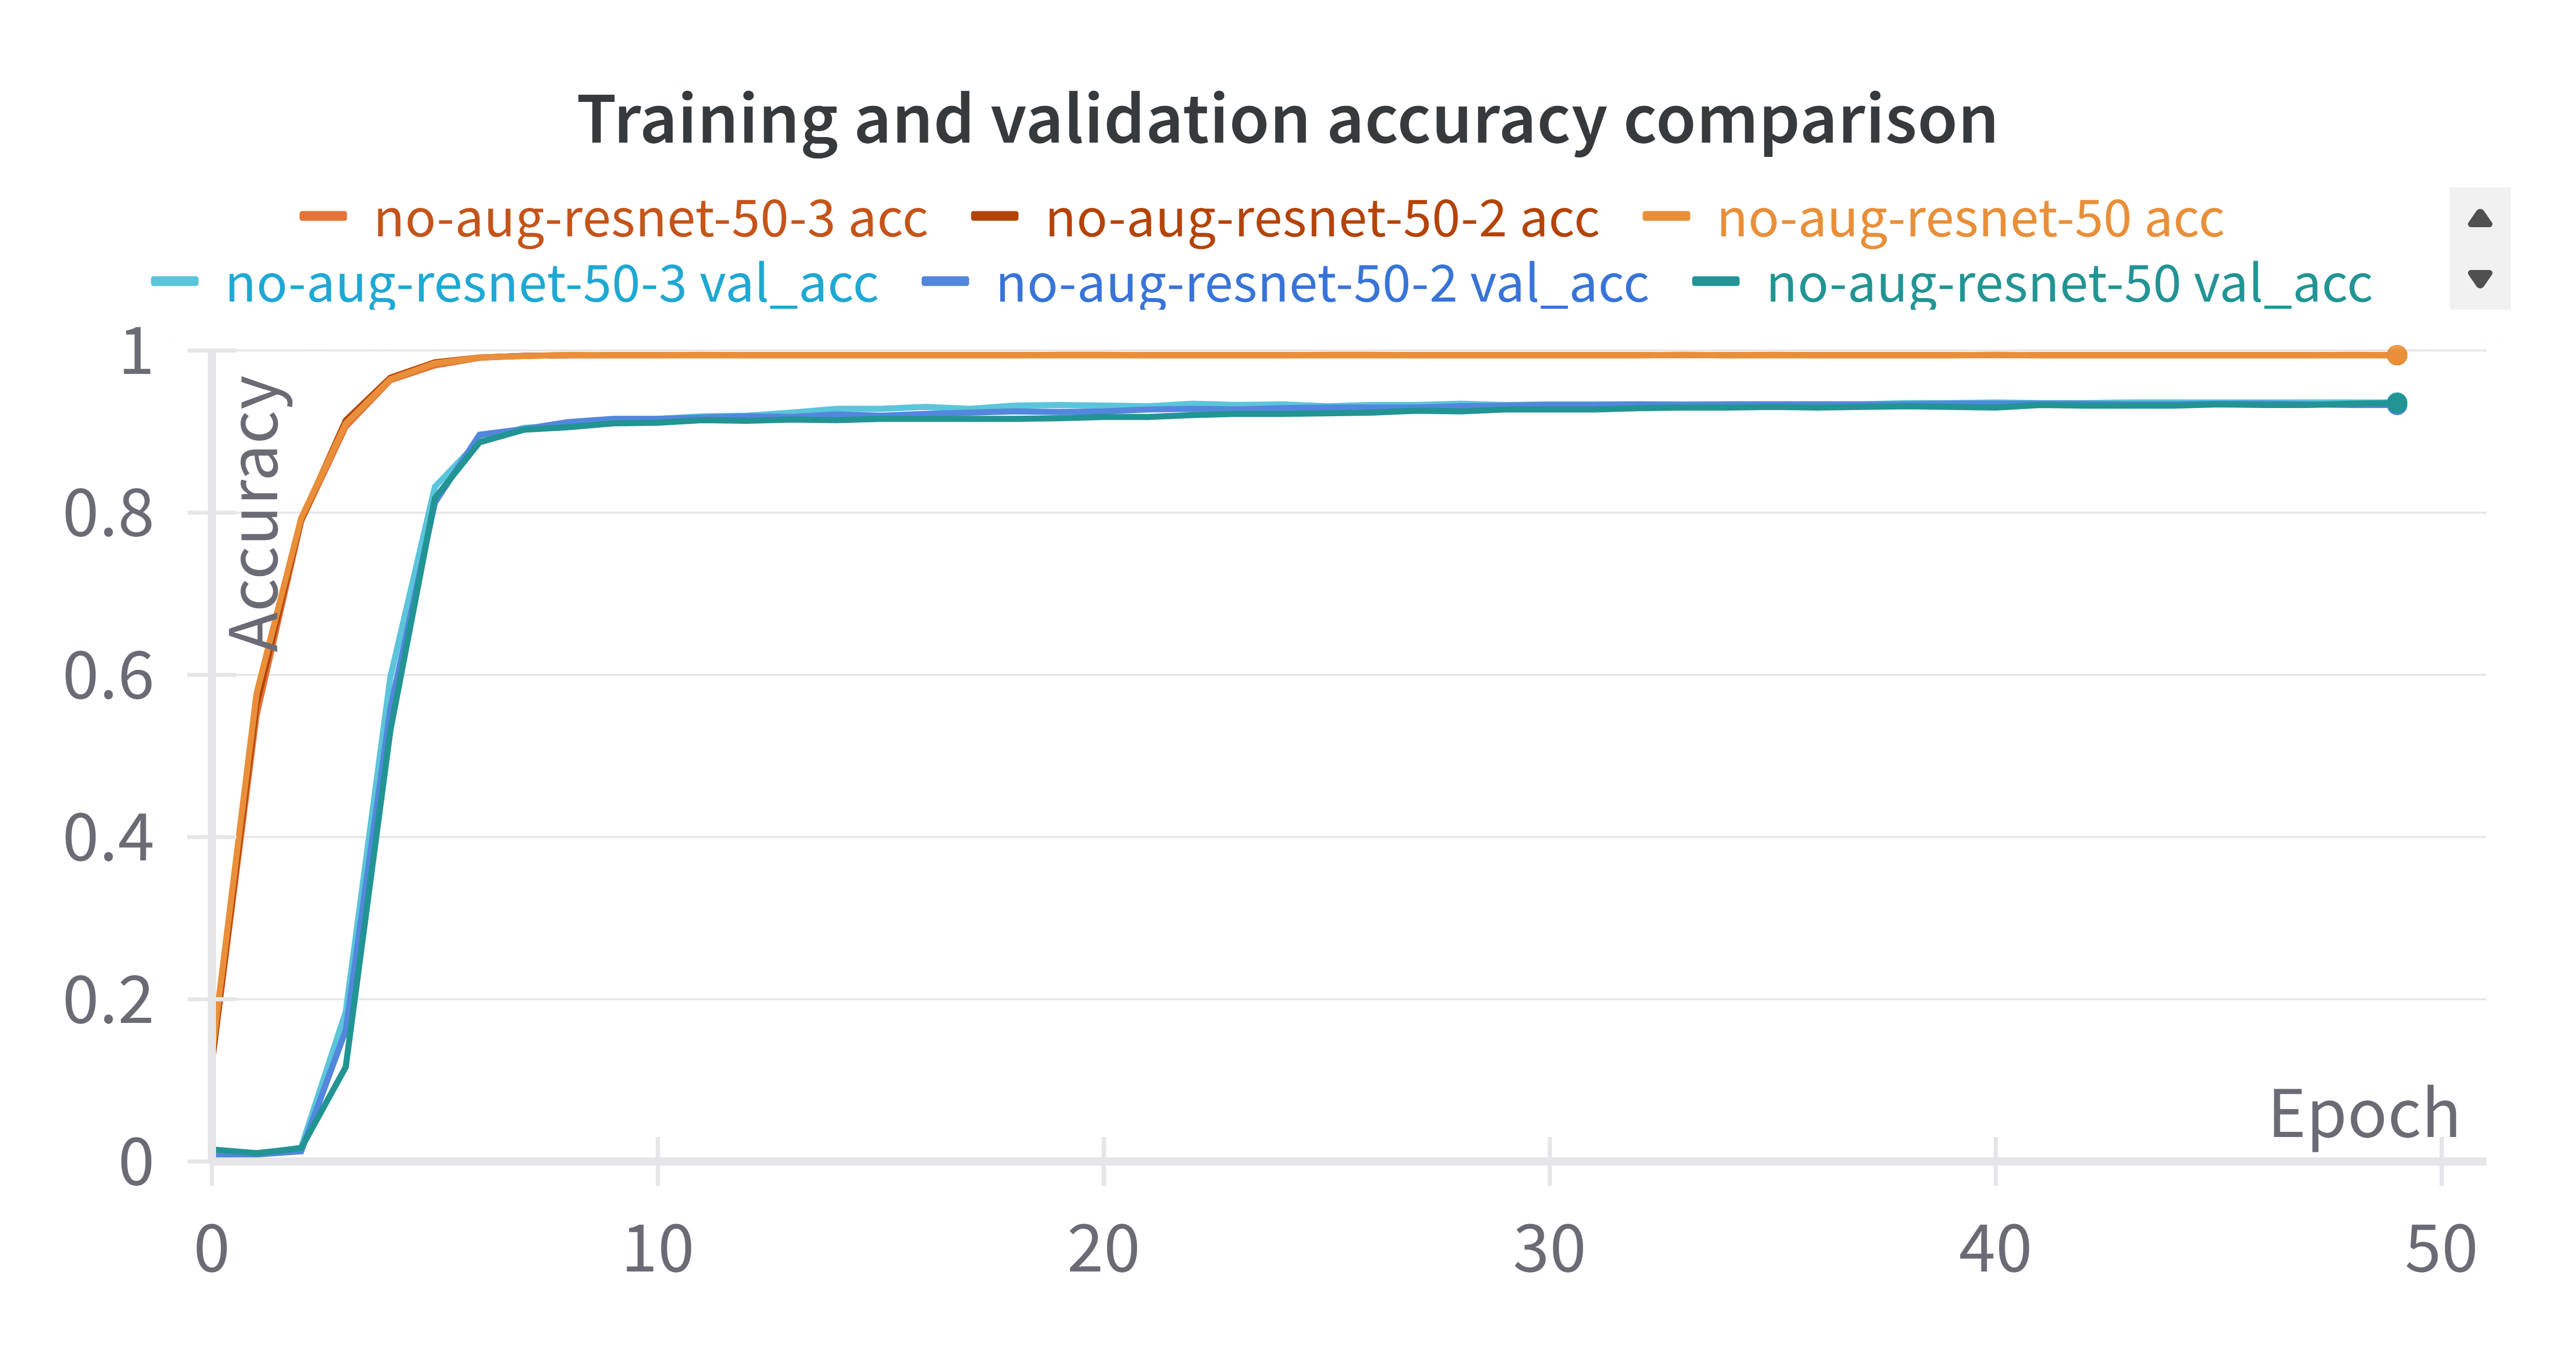
\includegraphics[width=0.95\textwidth]{Images/flowers-results/Flowers-no-aug-acc.png}
        \caption{Training vs Validation Accuracy}
    \end{subfigure}
    \vspace{0.3cm}
    
    \begin{subfigure}{\textwidth}
        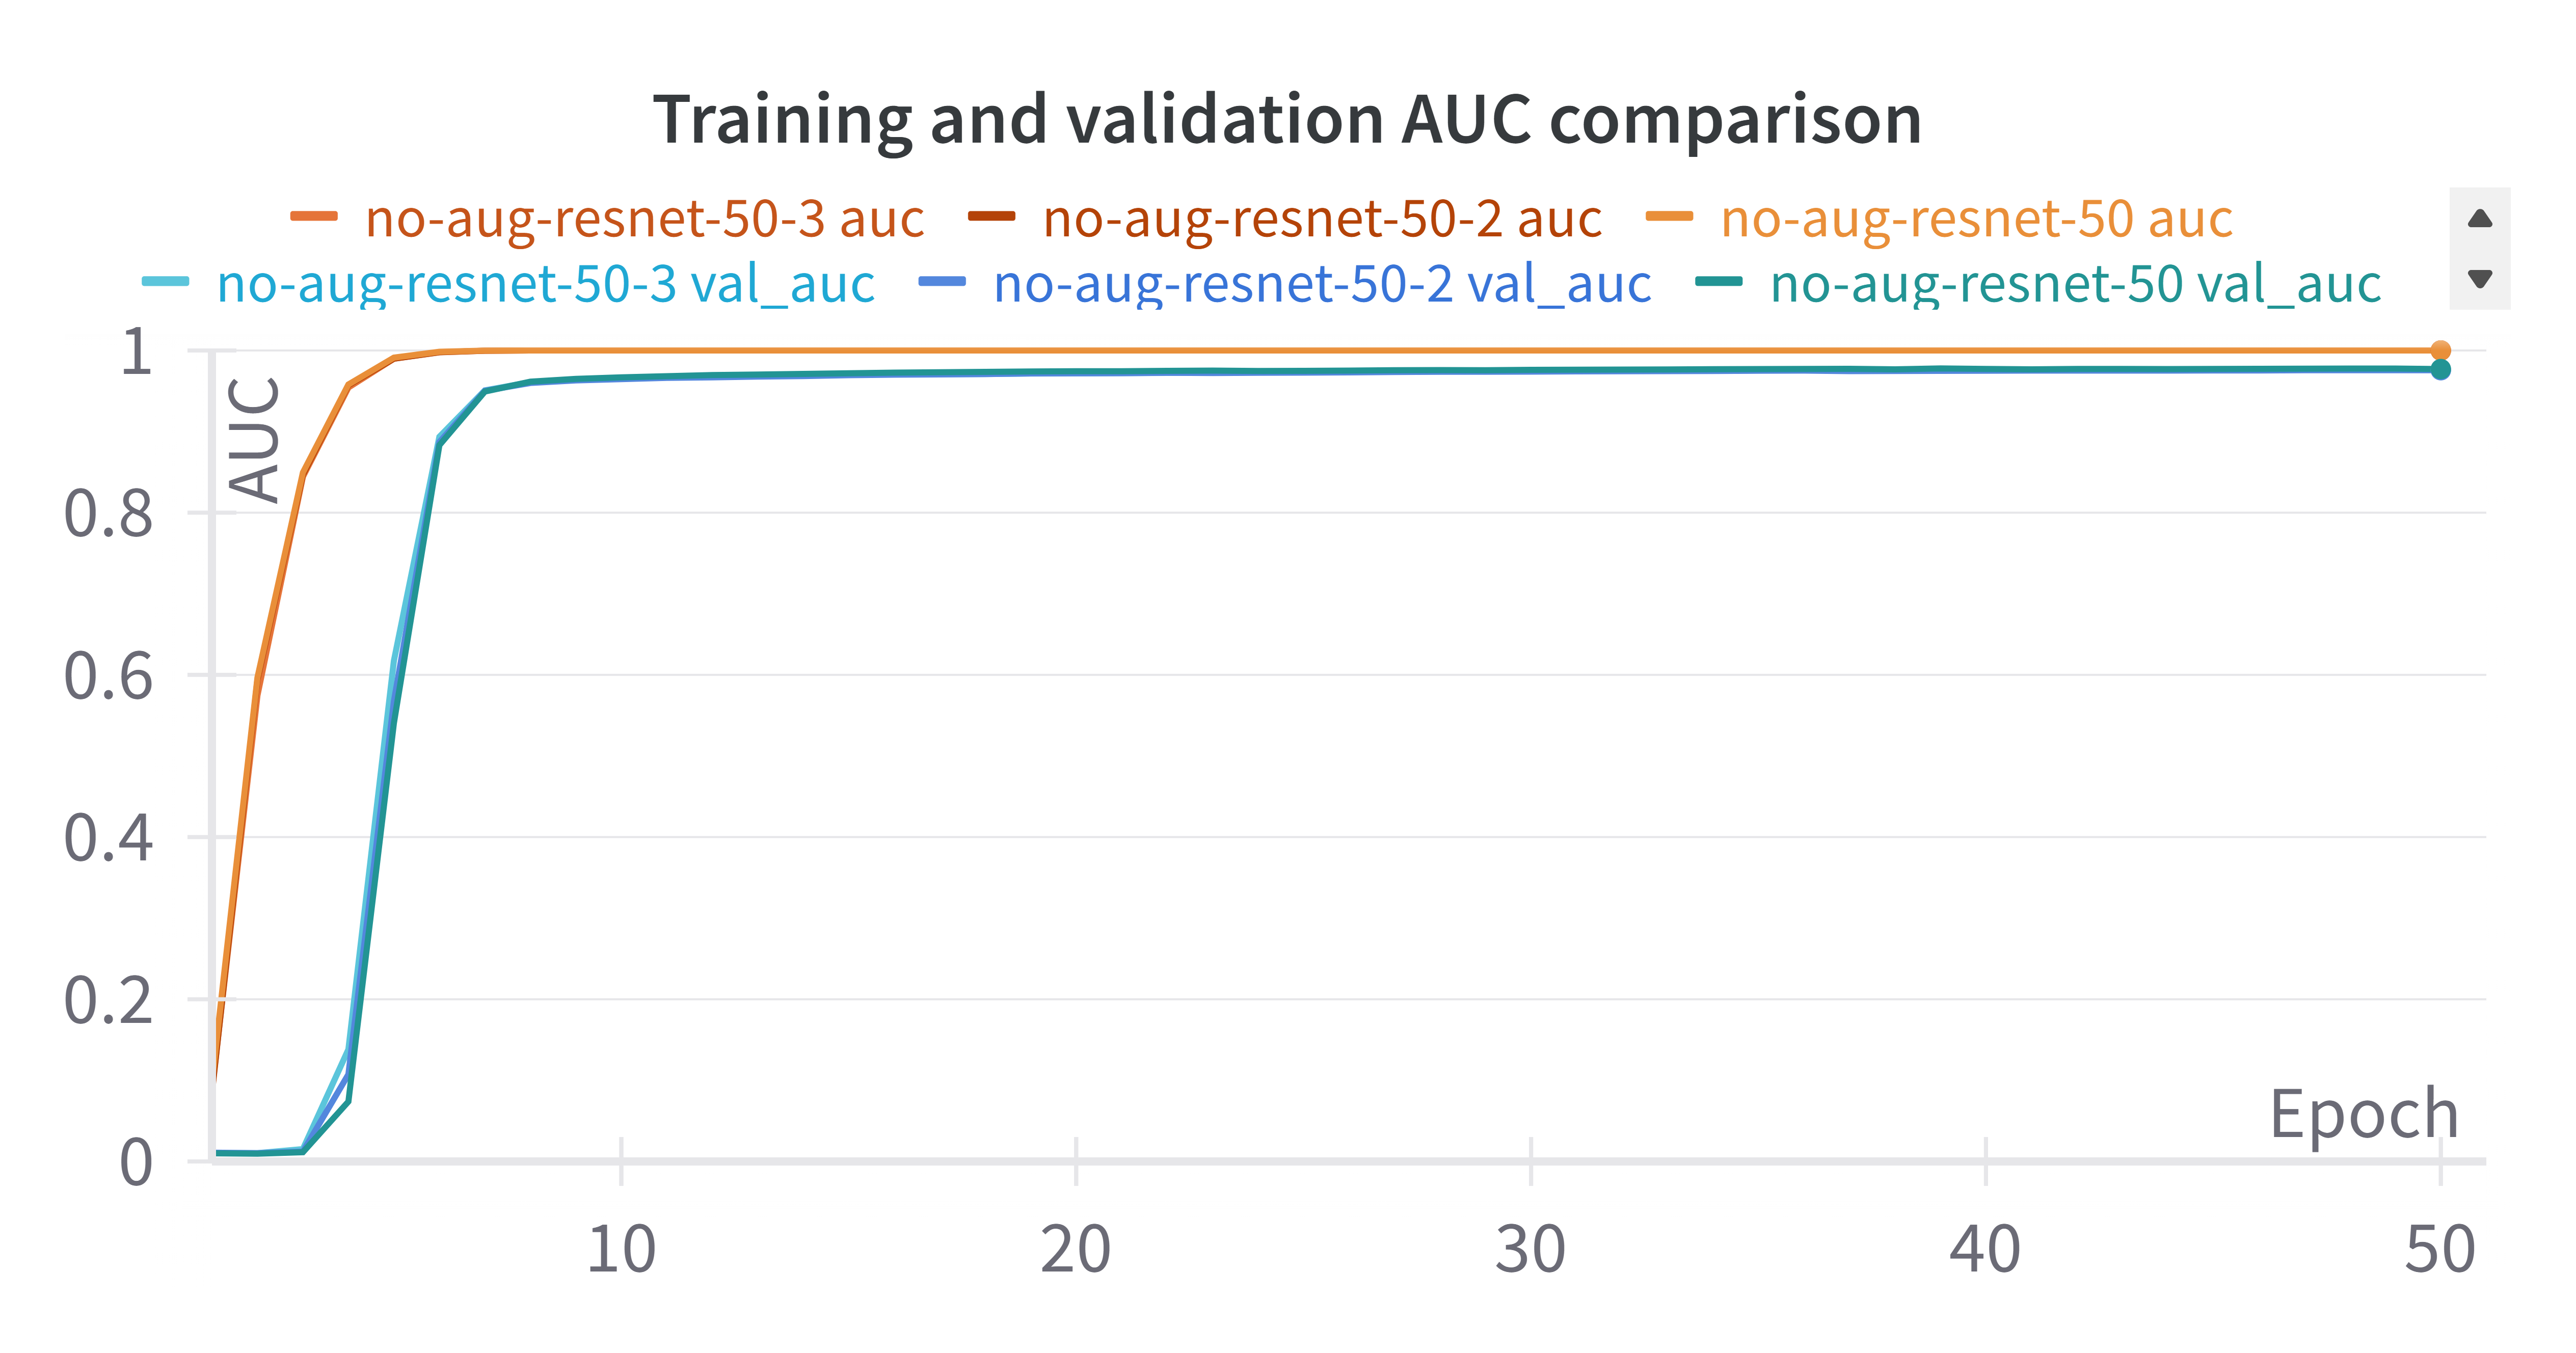
\includegraphics[width=0.95\textwidth]{Images/flowers-results/Flowers-no-aug-auc.png}\
        \caption{Training vs Validation AUC}
    \end{subfigure}
    \vspace{0.3cm}

    \caption{Learning curves for training and validation metrics without data augmentation.}
    \label{fig:flowersNoAug}
\end{figure}

The learning curves indicate that the model improves during the first 10 epochs but does not benefit significantly from further training. This experiment was repeated three times, producing consistent results in each trial.  Moreover, the model suffers overfitting, which becomes even more evident when examining Table \ref{tab:flowersNoAug}. The metrics for the best epoch show that both the training accuracy and AUC approach 1, indicating that the model is mainly memorizing the training data, which does not lead to achieving the highest possible level of generalization.

\begin{table}[h]
    \centering
    \caption{Performance metrics for the best epoch without data augmentation.}
    \begin{tabular}{|c|c|c|c|}
        \hline
        \textbf{Metric} & \textbf{Training} & \textbf{Validation}   \\ \hline
        Accuracy & 99.42 & 93.43 \\ \hline
        AUC & 1 & 0.974  \\ \hline
    \end{tabular}
    \label{tab:flowersNoAug}
\end{table}

Table \ref{tab:testFlowersNoAug} presents the performance metrics calculated on the test set. All values hover around 0.94, which is similar to the validation set metrics. To prevent the model from simply memorizing specific cases and to encourage it to learn more advanced features for effective classification, data augmentation techniques were employed.

\begin{table}[h]
    \centering
    \caption{Test Metrics for the best model without augmentation.}
    \label{tab:testFlowersNoAug}
    \begin{tabular}{|c|c|}
        \hline
        \textbf{Metric} & \textbf{Value} \\
        \hline
        Test Accuracy & 94.12 \\
        Precision & 94.03 \\
        Recall & 94.11 \\
        F1 Score & 93.87 \\
        \hline
    \end{tabular}
\end{table}

First, individual traditional data augmentation techniques were utilized and compared. The methods used at this stage include rotations by angles between -45 and 45 degrees, horizontal flipping, color adjustments (contrast and brightness), random zooming on parts of the input image, and the addition of Gaussian noise and Gaussian filtering. 

All augmentation techniques were carefully constrained to avoid unrealistic alterations of the flowers, such as excessive rotation, vertical flipping, extreme zoom, or overwhelming noise. This ensured that the flowers remained recognizable and reflective of their natural appearance. The results of these experiments are displayed in Table \ref{tab:testFlowersTradCompare}.

\begin{table}[b!]
\centering
\caption{Traditional augmentation comparison.}
\begin{tabular}{| >{\centering\arraybackslash}m{2.5cm} ! {\vrule width 1.5pt} >{\centering\arraybackslash}m{1.0cm} | >{\centering\arraybackslash}m{1.0cm} !{\vrule width 1.5pt} >{\centering\arraybackslash}m{1.0cm} | >{\centering\arraybackslash}m{1.0cm} !{\vrule width 1.5pt} >{\centering\arraybackslash}m{1.0cm} | >{\centering\arraybackslash}m{1.0cm} | >{\centering\arraybackslash}m{1.0cm} | >{\centering\arraybackslash}m{1.0cm} |}
\hline
\multirow{2}{*}{\textbf{Augmentation}} & \multicolumn{2}{c!{\vrule width 1.5pt}}{\textbf{Train}} & \multicolumn{2}{c!{\vrule width 1.5pt}}{\textbf{Val}} & \multicolumn{4}{c|}{\textbf{Test}} \\
\cline{2-9}
 & \textbf{Acc} & \textbf{AUC} & \textbf{Acc} & \textbf{AUC}  & \textbf{Acc} & \textbf{Prec.} & \textbf{Recall} & \textbf{F1} \\
\hline
no-aug & 99.42 & 1 & 93.43 & 0.976 & 94.12 & 94.03 & 94.12 & 93.84 \\
\hline
flip & 99.42 & 1 & 94.84 & 0.982 & 94.99 & 94.83 & 94.99 & 94.75 \\
\hline
\textbf{cropping} & 99.42 & 1 & \textbf{95.23} & \textbf{0.981} & 95.60 & 95.39 & 95.60 & 95.35 \\
\hline
\textbf{rotate45}  & \textbf{99.39} & 1 & 94.92 & 0.981 & \textbf{95.91} & \textbf{95.62} & \textbf{95.91} & \textbf{95.62} \\
\hline
color & 99.42 & 1 & 93.75 & 0.978 & 94.99 & 94.86 & 94.99 & 94.62 \\
\hline
gn-noise & 99.42 & 1 & 93.44 & 0.978 & 94.93 & 94.78 & 94.93 & 94.59 \\
\hline
gn-filter & 99.42 & 1 & 94.14 & 0.978 & 94.93 & 94.80 & 94.93 & 94.65 \\
\hline
\end{tabular}
\label{tab:testFlowersTradCompare}
\end{table}

To begin with, we can see that traditional data augmentation techniques used in this experiment did not impact the training accuracy and AUC values. However, there was a noticeable improvement in the validation and test metrics for every augmentation technique applied. 

For the validation set, most accuracy values, except Gaussian noise augmentation, increased by one percentage point, which is significant, considering the initial validation accuracy was 93.4\%. Notably, cropping had the best results, with the validation accuracy increasing to 95.2\%, a rise of 1.8\%.

Similar improvements were observed in the test set metrics. The baseline accuracy without augmentation was 94.1\%. This value increased with every augmentation technique. Specifically, the accuracy improved by approximately 1.5 and 1.8 percentage points for \textbf{rotation} and \textbf{cropping}, respectively.

As mentioned before, despite the increased validation and test set metrics, the application of these augmentation methods individually did not decrease the training set metrics values, which remained close to 100\%. The next step involved investigating whether combining all augmentation techniques, with varying probabilities of application, could make the training set more challenging. This approach aimed to potentially decrease the model's performance on the training data while further improving validation and test set results.

Figure \ref{fig:flowersLCAugComparison} presents a comparison of the training and validation accuracy learning curves under three conditions: without data augmentation, with all traditional augmentations applied, and with advanced augmentation, which includes all types of augmentations, such as \textit{CutMix} and \textit{MixUp}.

\begin{figure}[!htb]
    \centering
    \begin{subfigure}{0.95\textwidth}
        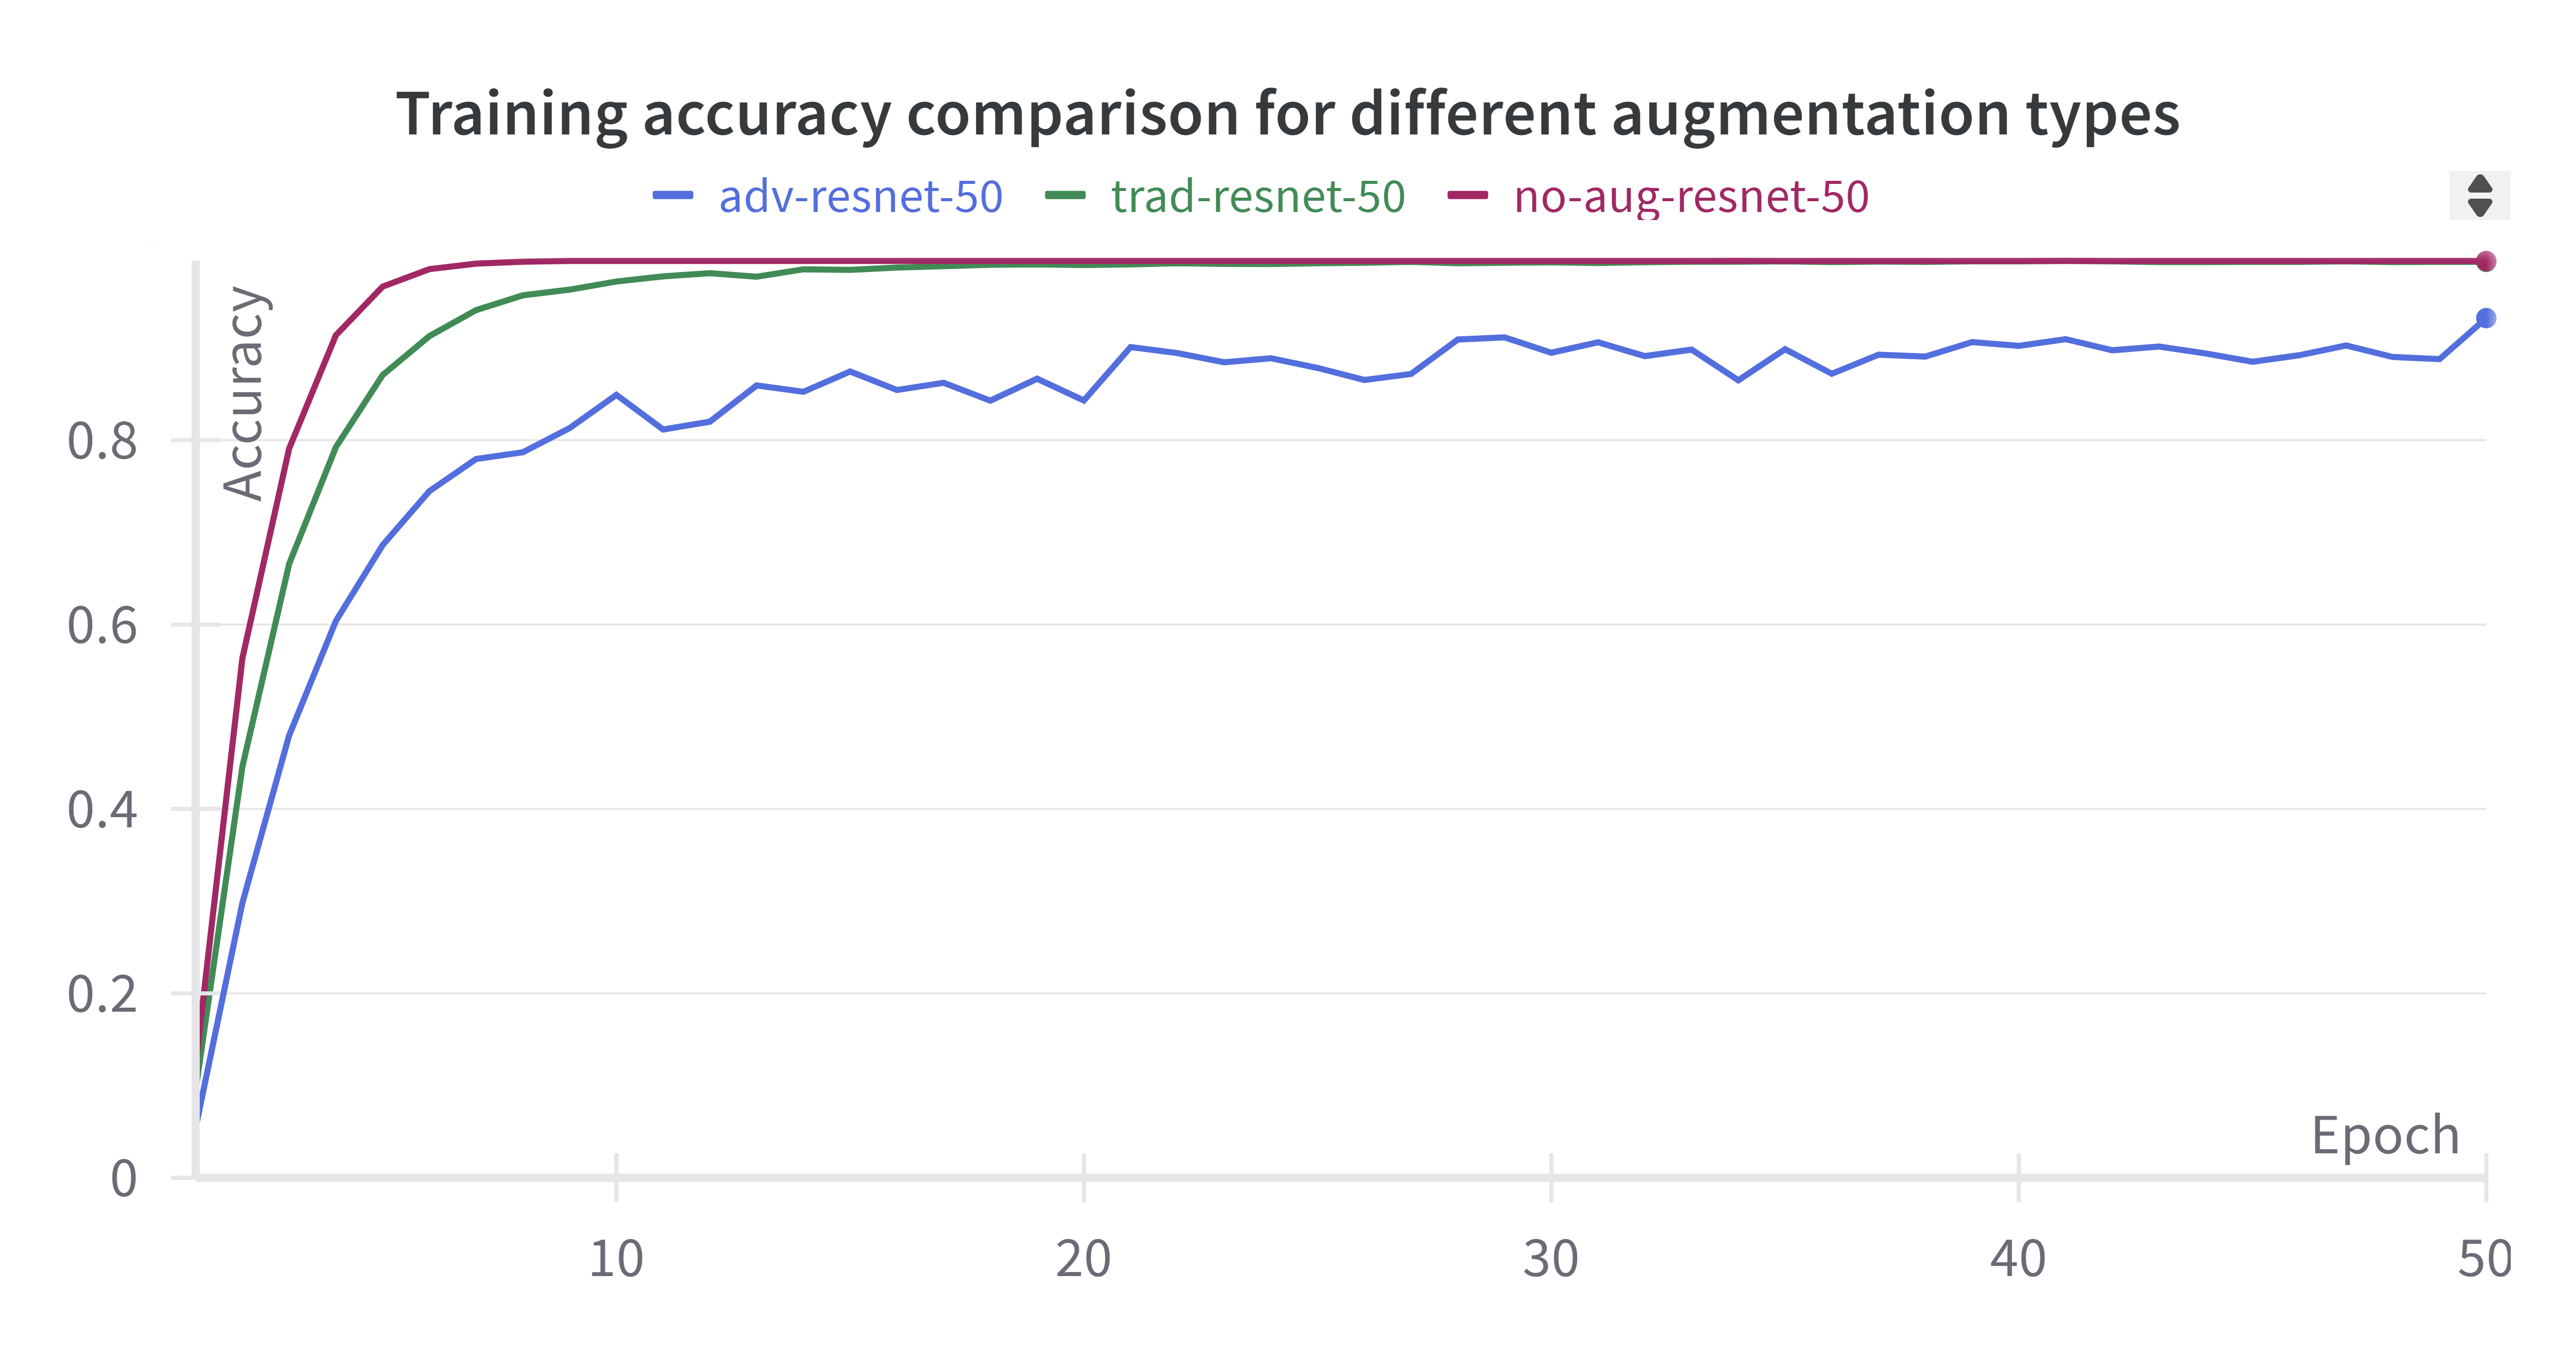
\includegraphics[width=\textwidth]{Images/flowers-results/Learning-Curves-Train-Aug-Comparison.png}
        \caption{Training Accuracy}
    \end{subfigure}
    \vspace{0.3cm}

    \begin{subfigure}{0.95\textwidth}
        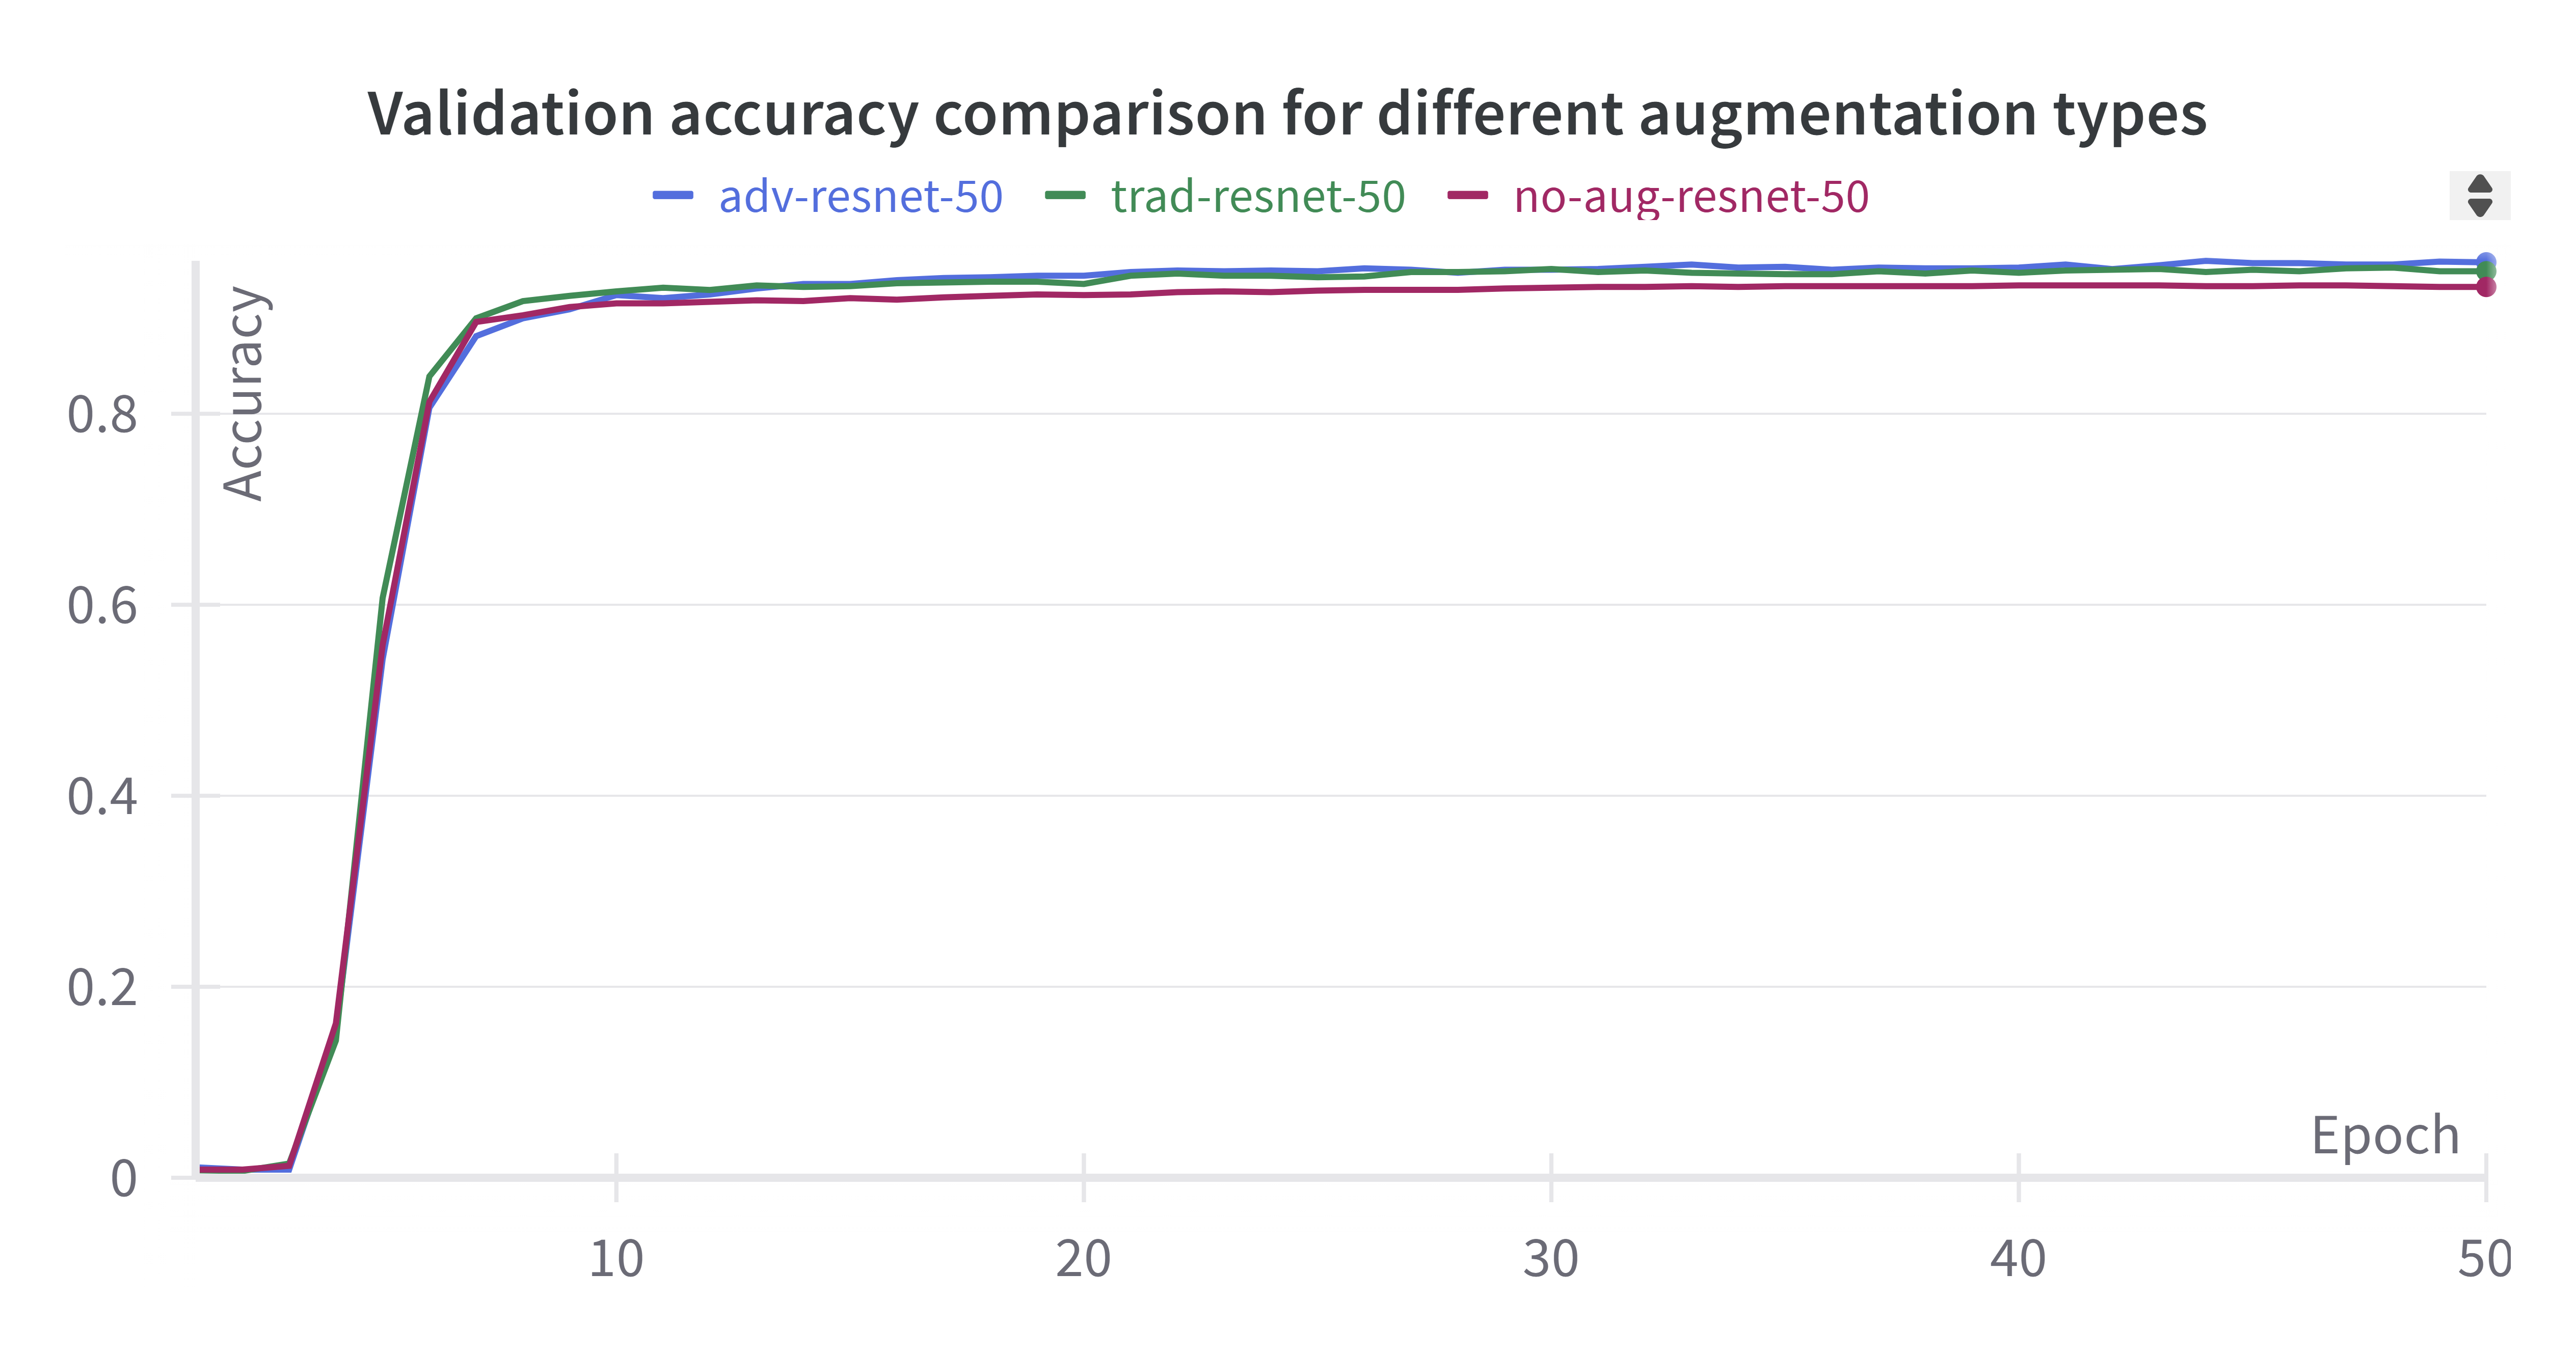
\includegraphics[width=\textwidth]{Images/flowers-results/Learning-Curves-Val-Aug-Comparison.png}\
        \caption{Validation Accuracy}
    \end{subfigure}
    \vspace{0.3cm}
    \caption{Training and validation accuracy learning curves comparison for different augmentation types.}
    \label{fig:flowersLCAugComparison}
\end{figure}

The best validation results are achieved by combining all data augmentation techniques together, referred to as \textbf{adv-resnet-50} on the plot. Although the difference is minimal, traditional augmentation techniques yield slightly lower performance. In contrast, the absence of augmentation techniques results in worse generalization, where the model's performance on the training set does not translate effectively to the validation and test sets.

\begin{figure}[!h]
    \centering
    \begin{subfigure}{0.75\textwidth}
        \centering
        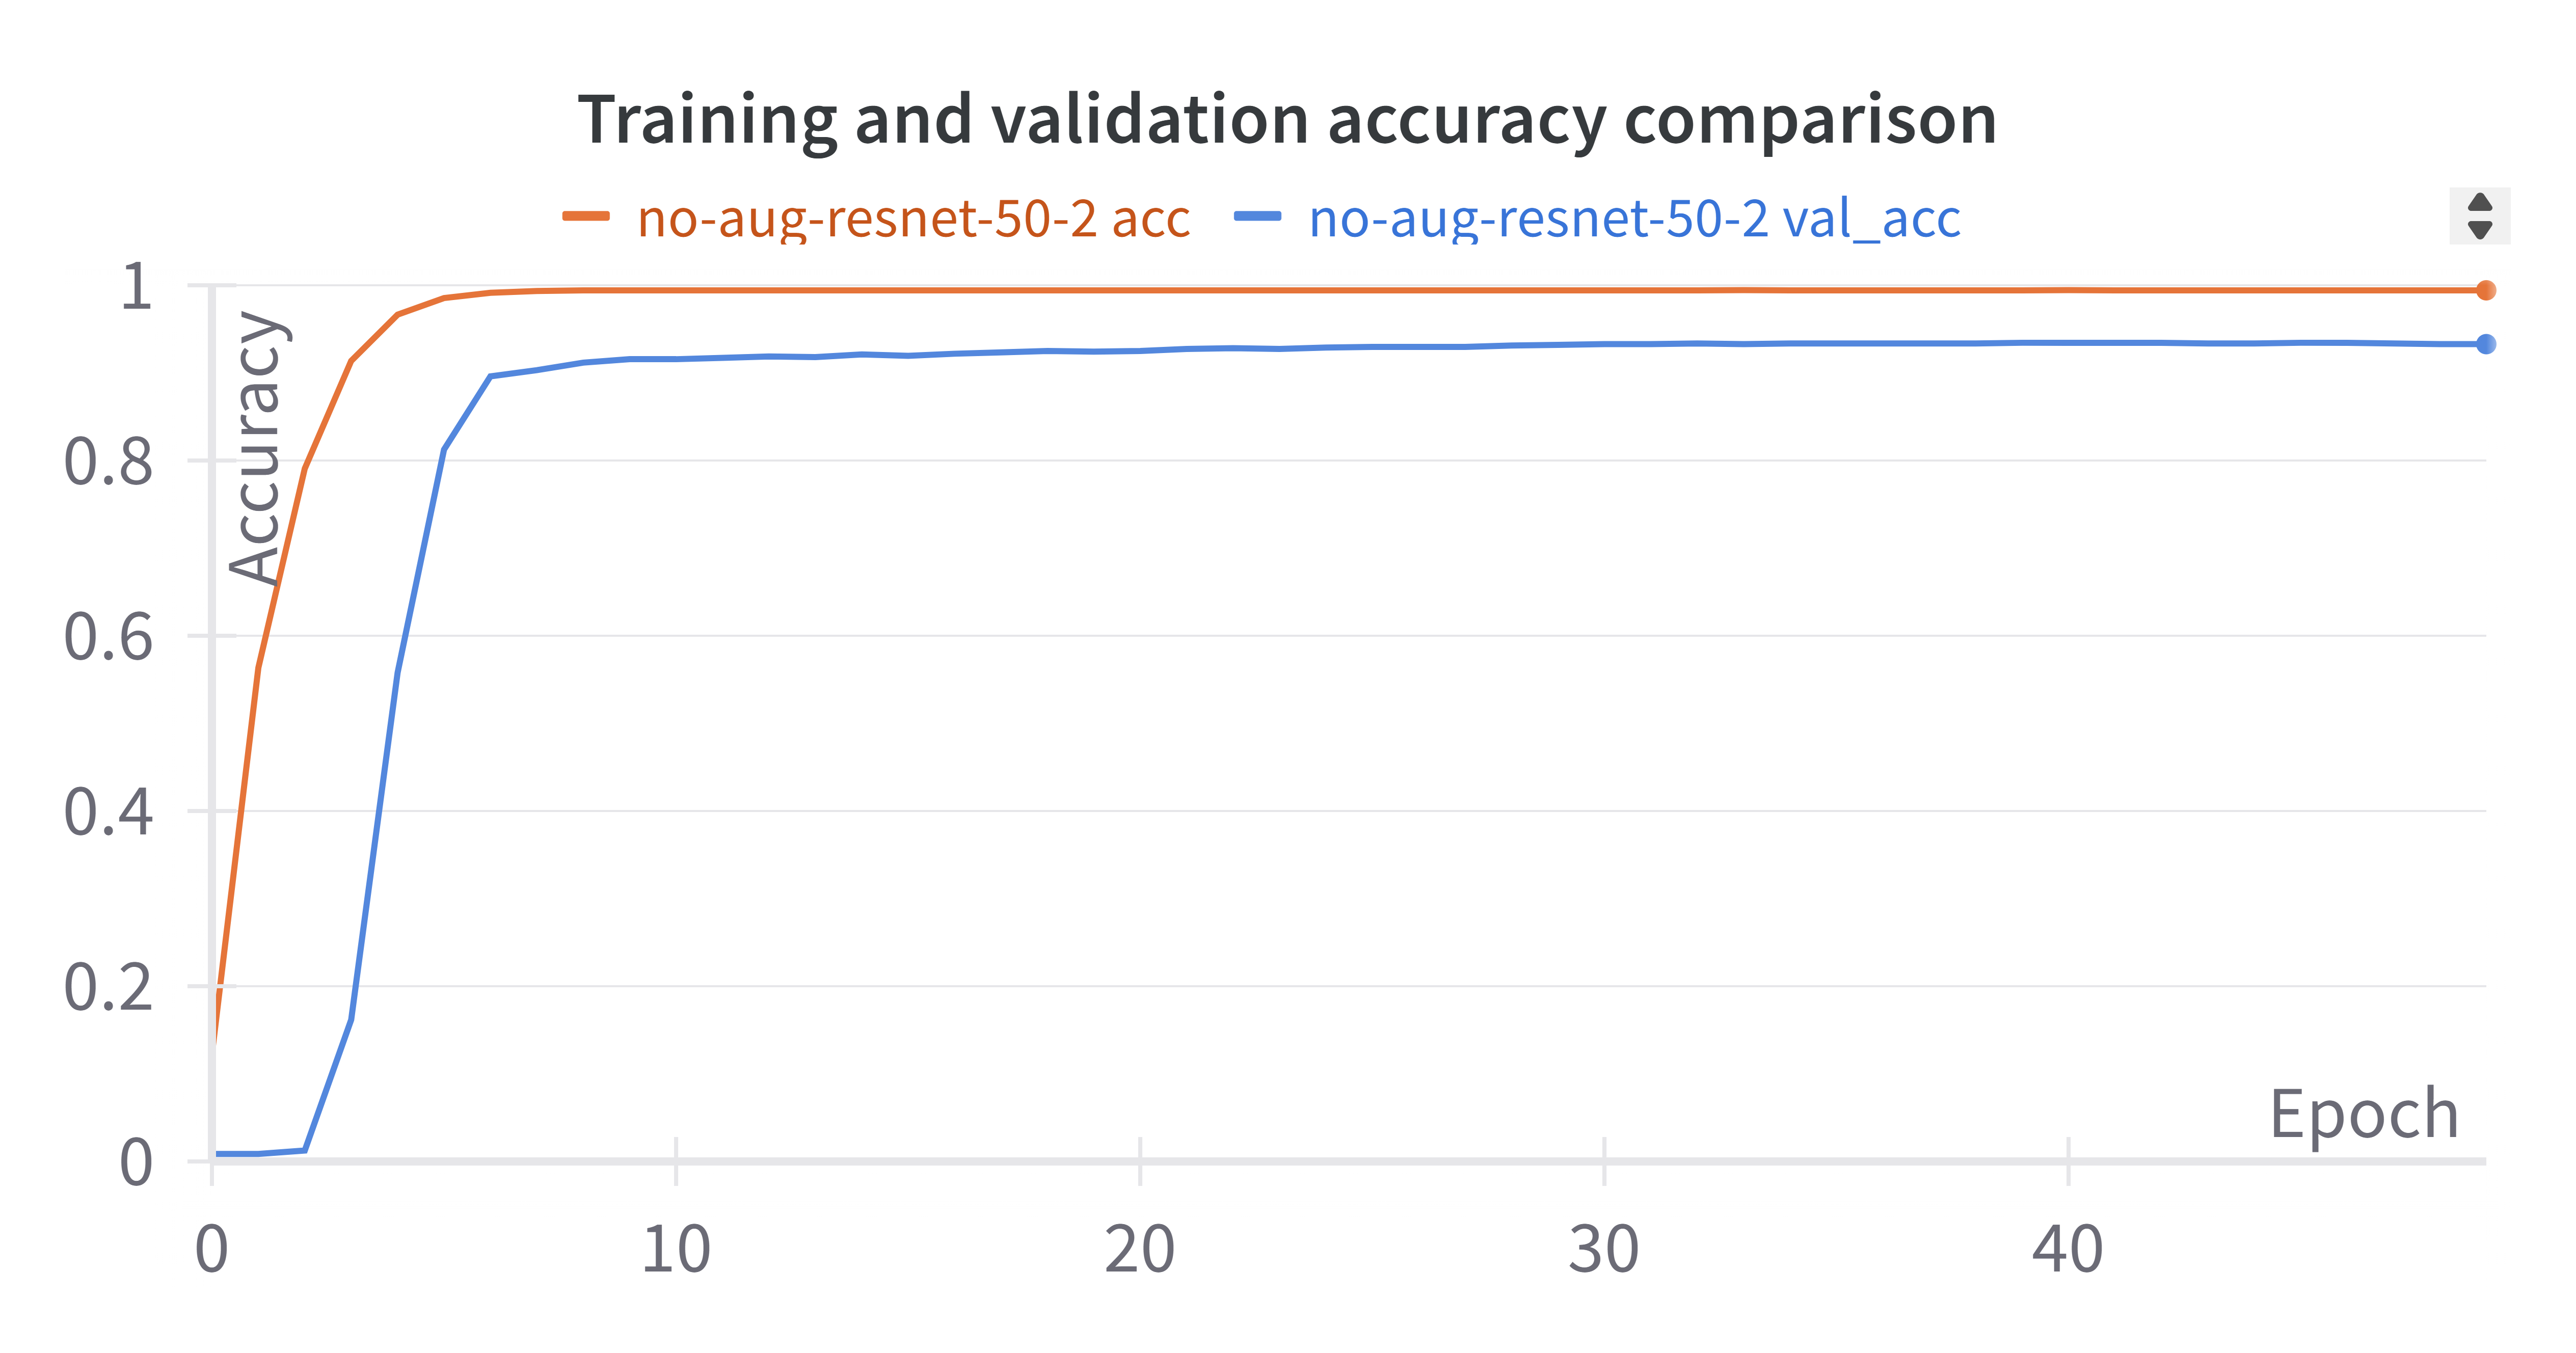
\includegraphics[width=\textwidth]{Images/flowers-results/LC-Train-Val-No-Aug.png}
        \caption{No Augmentation}
    \end{subfigure}
    \vspace{0.3cm}

    \begin{subfigure}{0.75\textwidth}
        \centering
        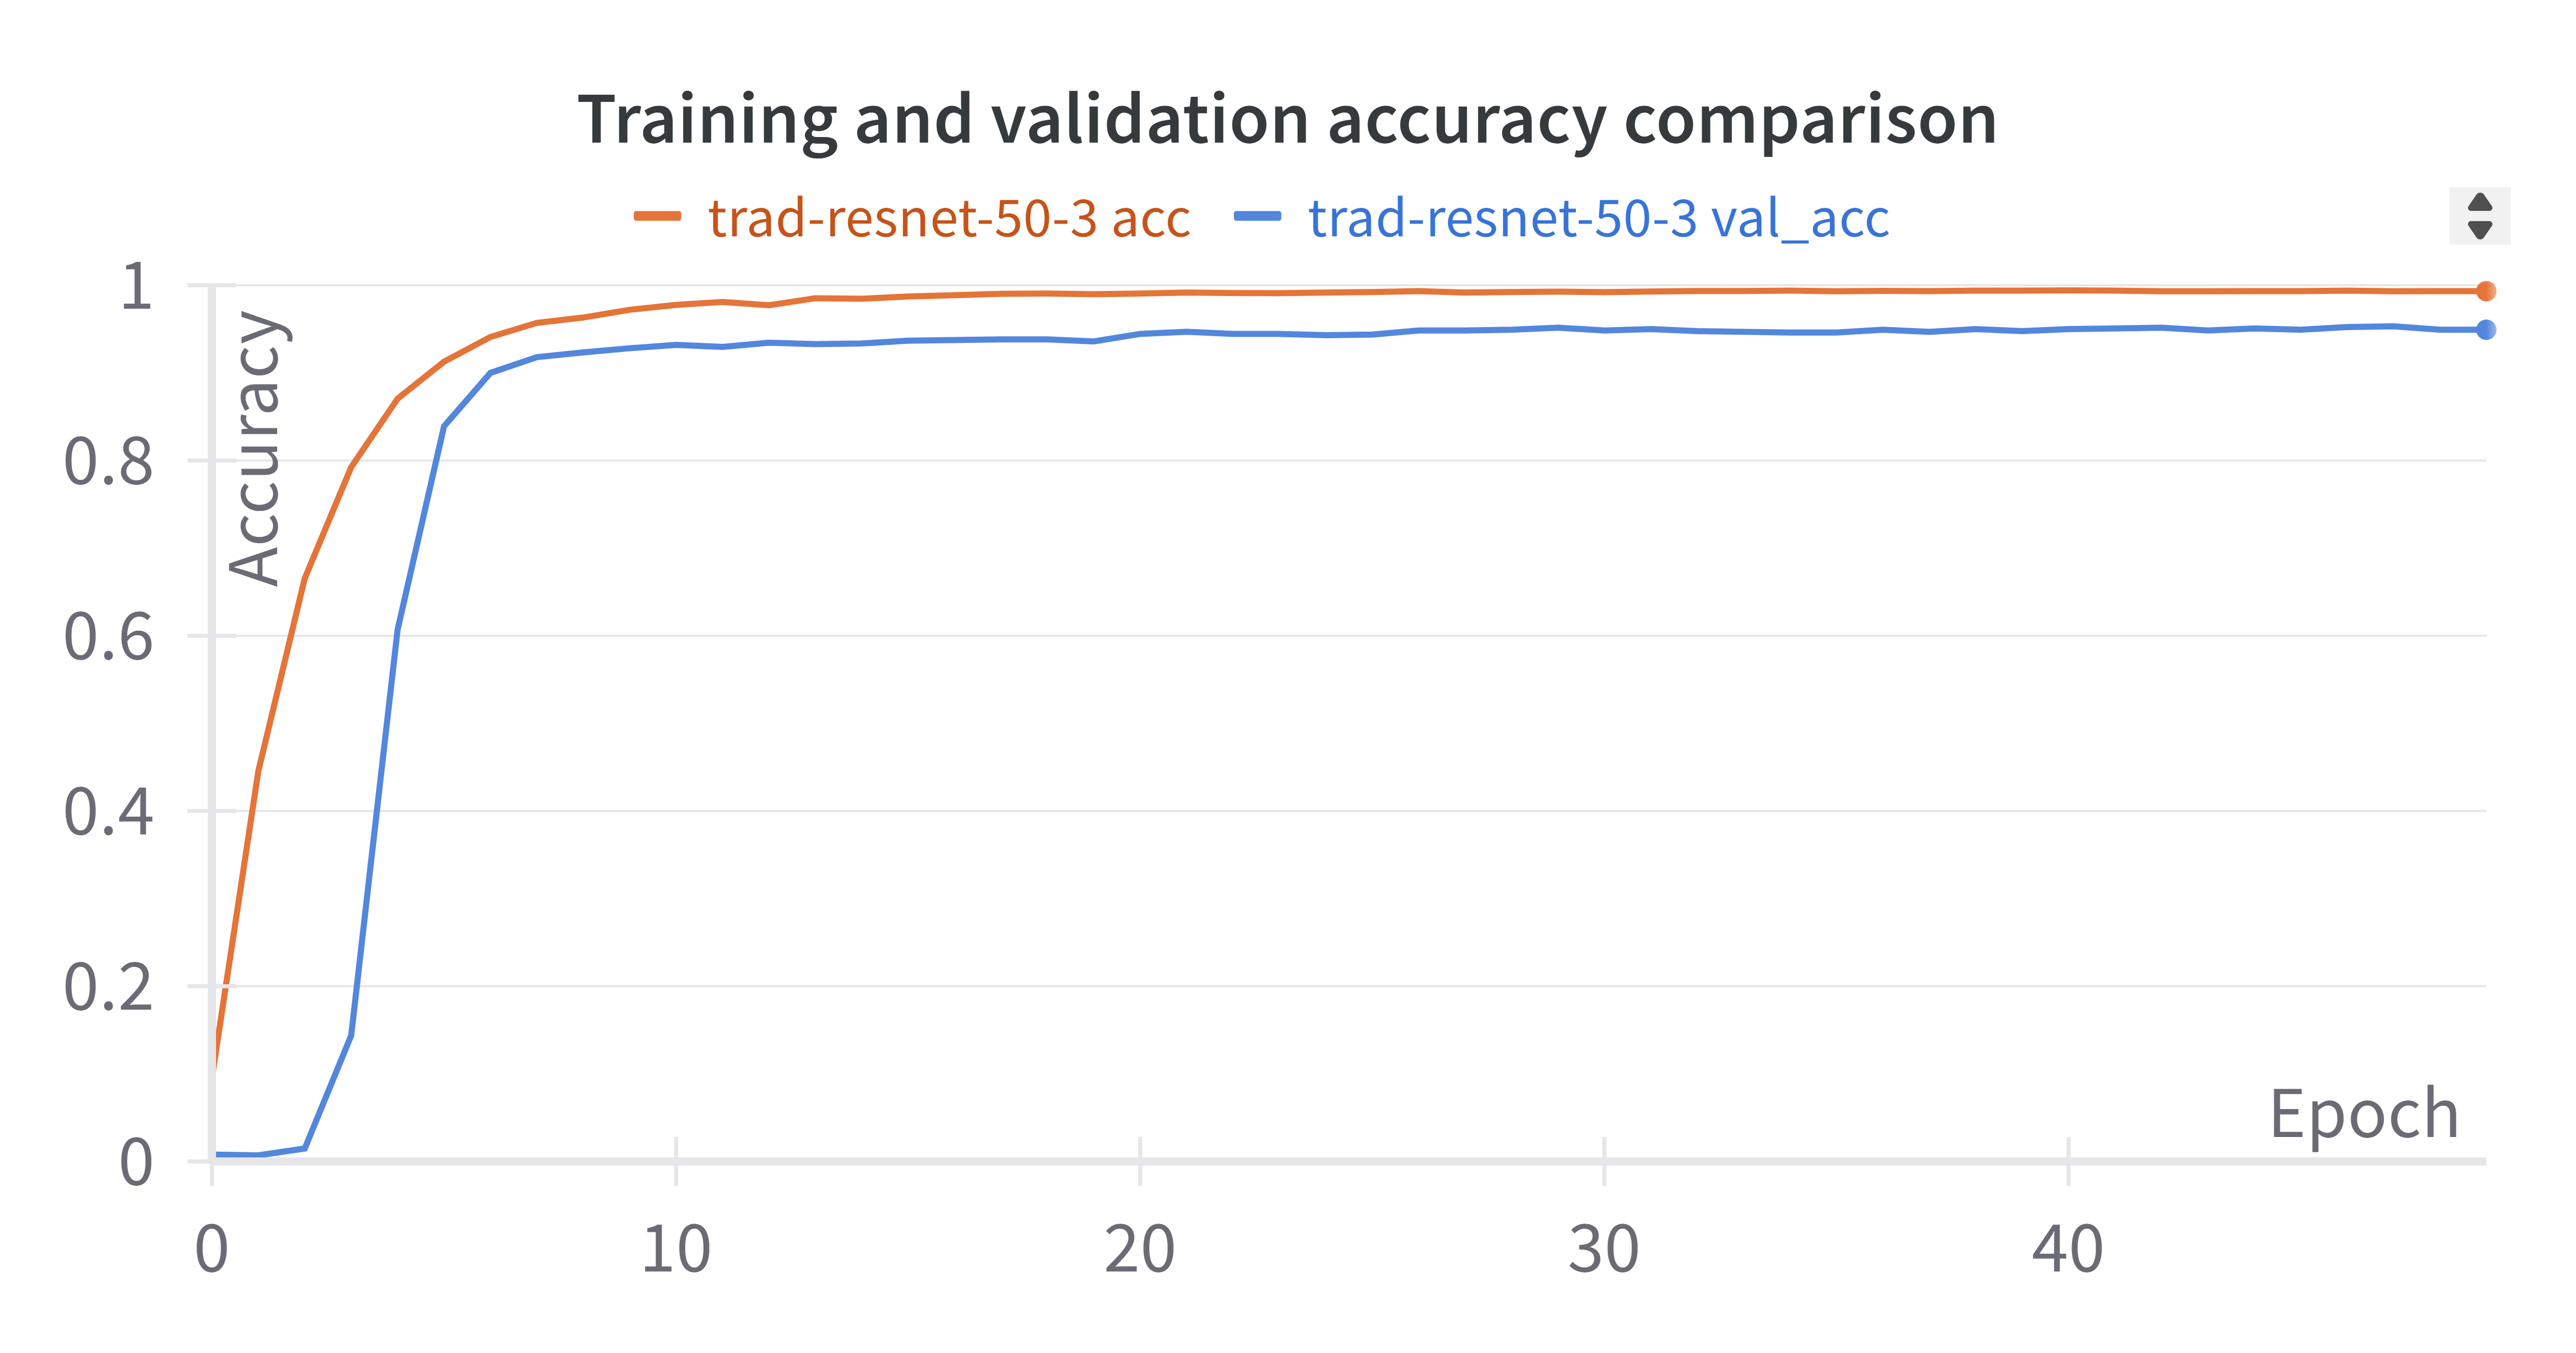
\includegraphics[width=\textwidth]{Images/flowers-results/LC-Train-Val-Trad-Aug.png}\
        \caption{Traditional Augmentation}
    \end{subfigure}
    \vspace{0.3cm}

    \begin{subfigure}{0.75\textwidth}
        \centering
        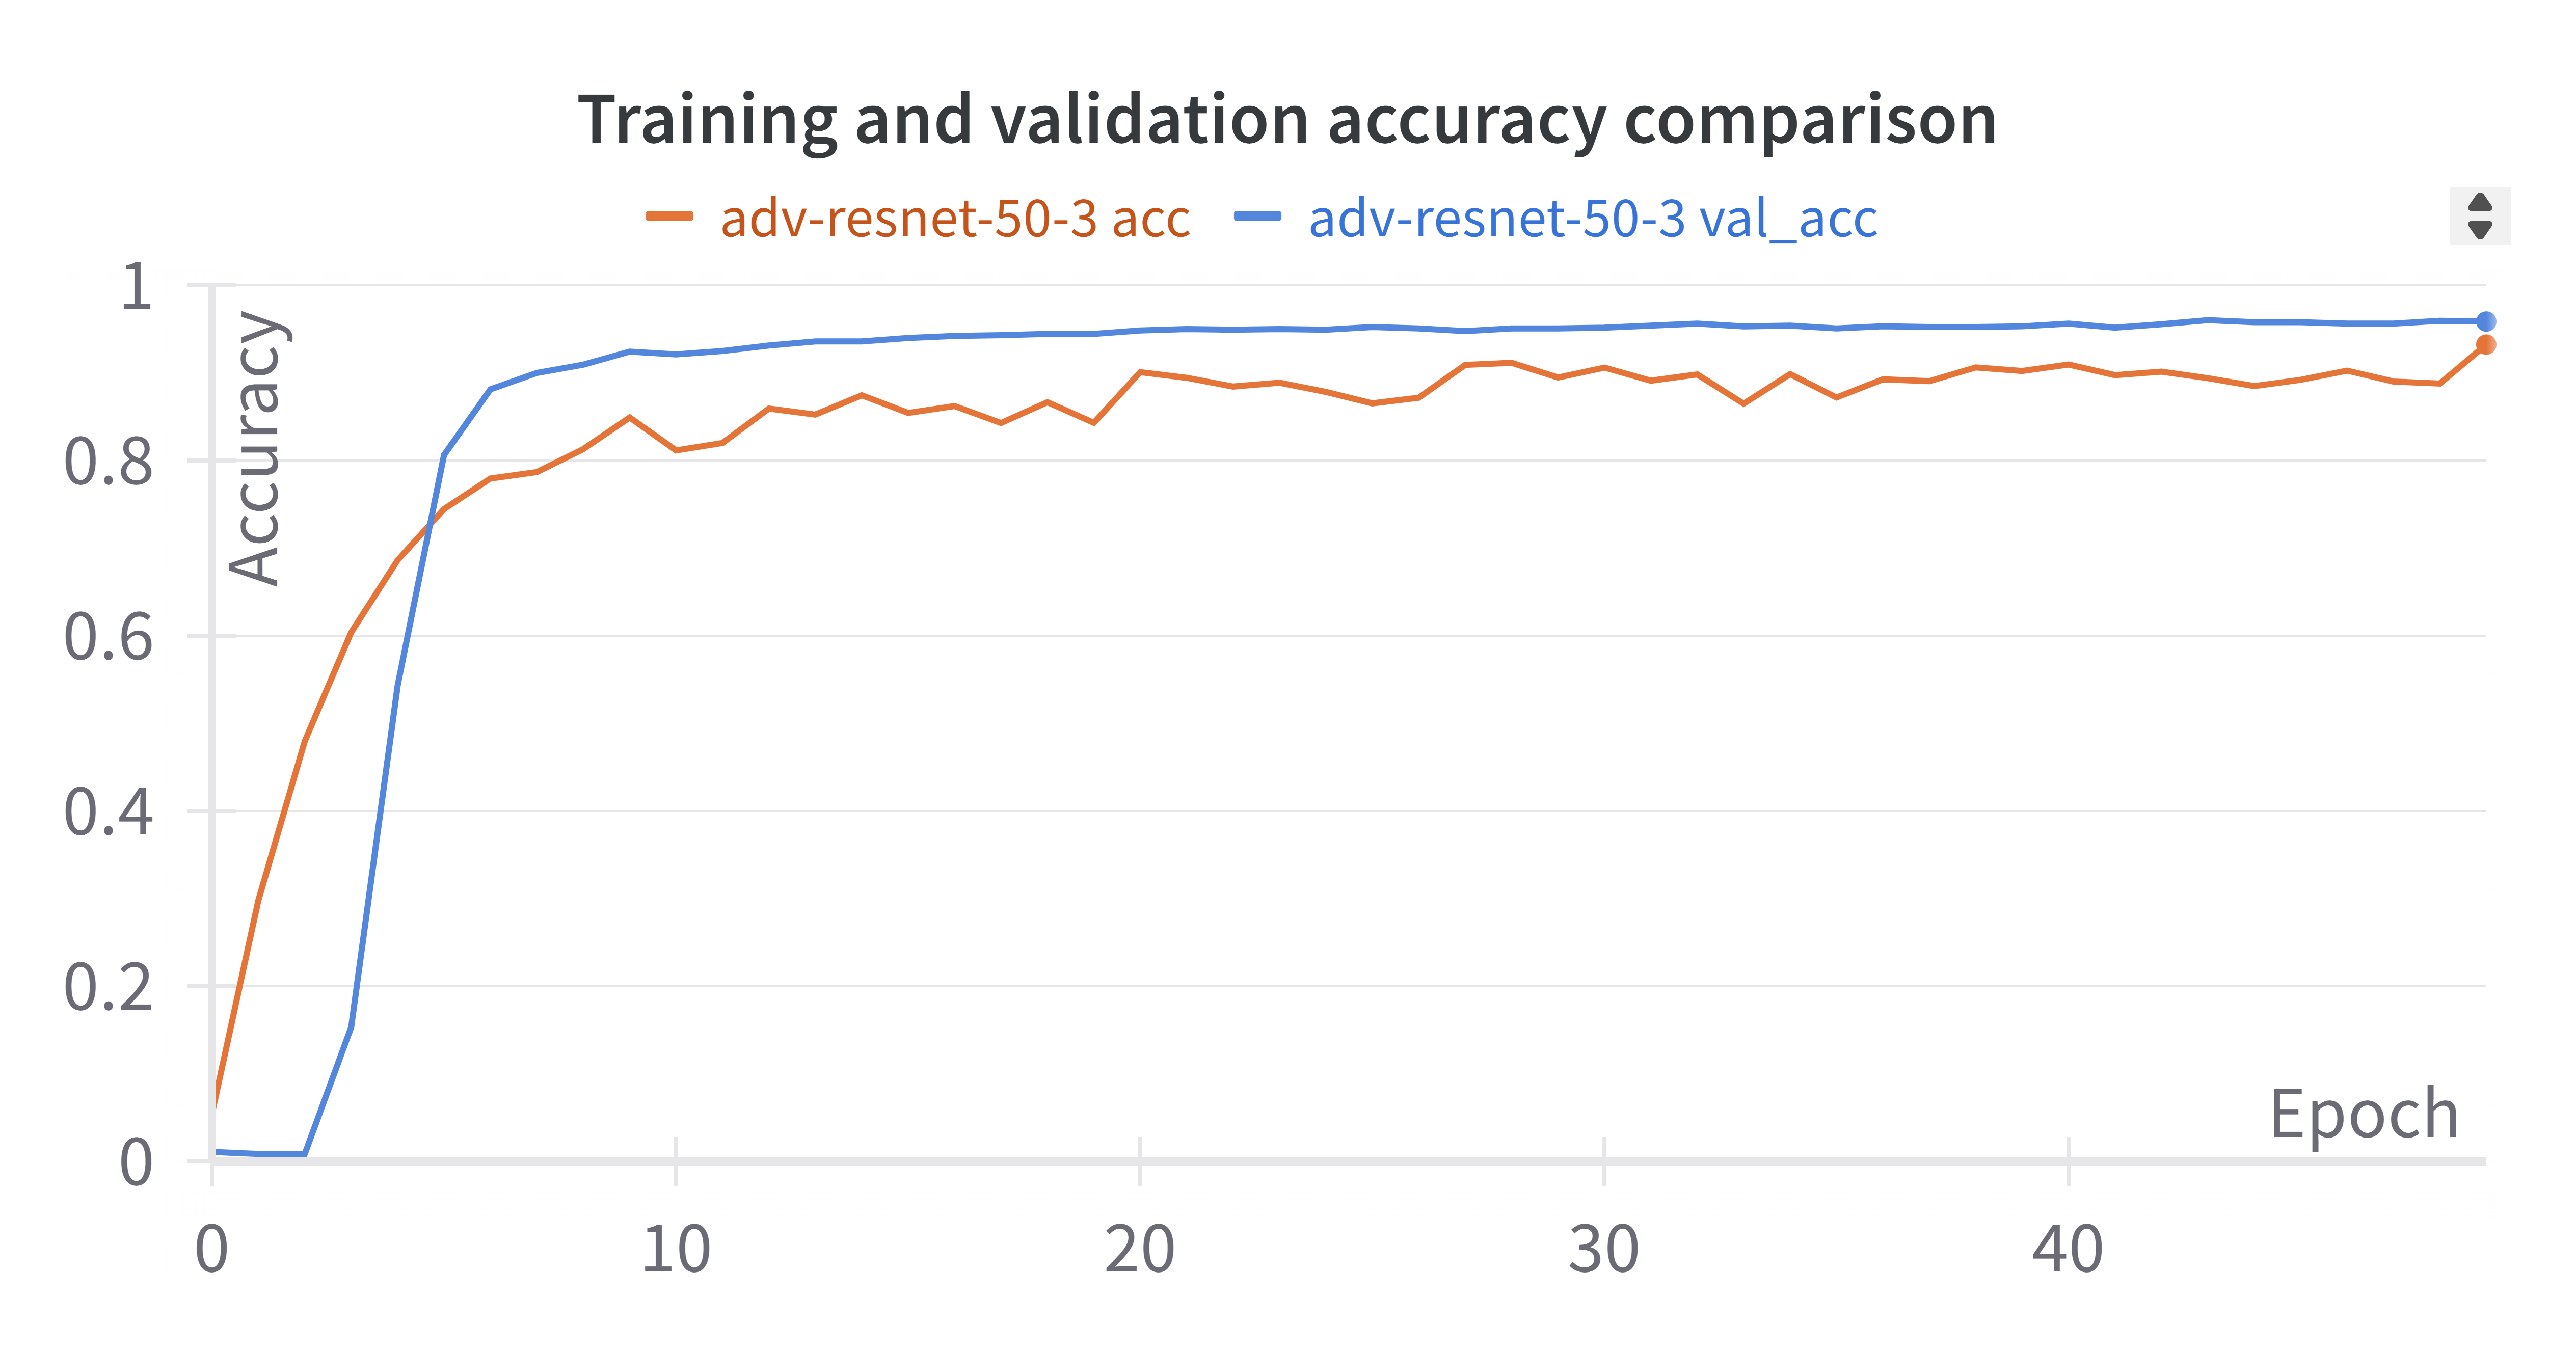
\includegraphics[width=\textwidth]{Images/flowers-results/LC-Train-Val-Adv-Aug.png}
        \caption{Advanced Augmentation}
    \end{subfigure}
    \vspace{0.3cm}

    \caption{Learning Curves for each augmentation technique separately.}
    \label{fig:LCSeparately}
\end{figure}

Figure \ref{fig:LCSeparately} shows comparison of learning curves -- training and validation -- separately, for each augmentation technique described above. It is important to note that when data augmentation is used, the training dataset becomes much more challenging, and the point where the values of training metrics are lower than the values of validation and test metrics is achieved. This indicates that the model has \textbf{difficulty accurately classifying training examples}, but through this challenge, \textbf{it learns advanced features that improve its ability to recognize simpler validation and test examples} not encountered during parameter updates. The numerical values of the learning curves described above are shown in Table \ref{tab:FlowersBestEpoch}.

\begin{table}[h!]
\centering
\caption{Accuracy and AUC metrics for the best epoch using combined augmentation techniques.}
\begin{tabular}{| >{\centering\arraybackslash}m{2.5cm} !{\vrule width 1.5pt} >{\centering\arraybackslash}m{1.0cm} | >{\centering\arraybackslash}m{1.0cm} !{\vrule width 1.5pt} >{\centering\arraybackslash}m{1.0cm} | >{\centering\arraybackslash}m{1.0cm} !{\vrule width 1.5pt} }
\hline
\multirow{2}{*}{\textbf{Augmentation}} & \multicolumn{2}{c!{\vrule width 1.5pt}}{\textbf{Train}} & \multicolumn{2}{c!{\vrule width 1.5pt}}{\textbf{Val}} \\
\cline{2-5}
 & \textbf{Acc} & \textbf{AUC} & \textbf{Acc} & \textbf{AUC} \\
\hline
no-aug & 99.42 & 0.999 & 93.44 & 0.975 \\
\hline
trad-aug & 99.31 & 0.999 & 95.31 & 0.983 \\
\hline
adv-aug & 89.40 & 0.600 & 96.02 & 0.986 \\
\hline
\end{tabular}
\label{tab:FlowersBestEpoch}
\end{table}

Looking at the table above, we should pay attention to the training accuracy and AUC values for advanced augmentation. Although the training accuracy is 10 percentage points lower than that of other individual and combined augmentation methods, this does not imply poor performance on the validation and test sets. On the contrary, this network performs the best among all analyzed above.

Secondly, we can draw conclusions about the AUC metric. While traditional augmentation does not affect its value, advanced augmentation, which includes \textit{MixUp} and \textit{CutMix}, significantly lowers the training AUC while maintaining the highest validation AUC among the three methods. These techniques effectively implement a form of label smoothing by blending labels, which reduces the sharp boundaries between classes, making it more challenging for the model to maintain high separability. This leads to lower AUC values during training because the model is being trained on more ambiguous examples.  Consequently, the model learns more robust features, resulting in a high validation AUC.


Figure \ref{fig:testAllAug} shows a comparison of test metrics for models trained using various data augmentation techniques. It displays bar plots of the results from the best epoch for each technique. These results are consistent with the observations on the validation dataset. However, both augmentation methods show more noticeable improvements on the test set, with an increase of around 2 percentage points.

\begin{figure}[!htb]
    \centering
    \begin{subfigure}{0.45\textwidth}
        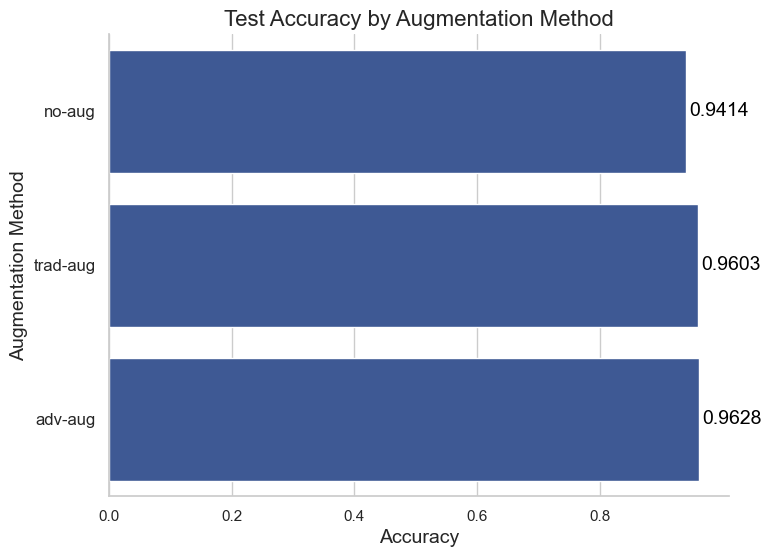
\includegraphics[width=\textwidth]{Images/flowers-results/test_acc.png}
        \caption{Accuracy}
    \end{subfigure}
    \vspace{0.3cm}
    \hfill
    \begin{subfigure}{0.45\textwidth}
        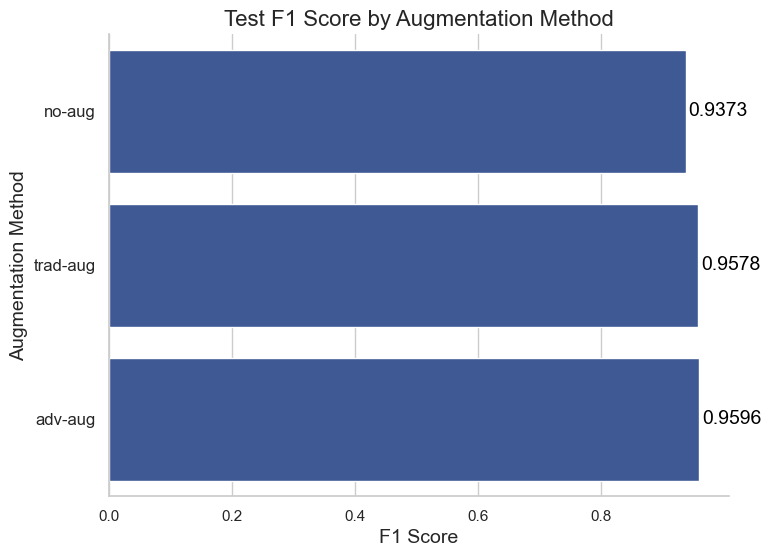
\includegraphics[width=\textwidth]{Images/flowers-results/test_f1.png}\
        \caption{F1 Score}
    \end{subfigure}
    \vspace{0.3cm}

    \caption{Test metrics for different types of data augmentation.}
    \label{fig:testAllAug}
\end{figure}

\newpage
Data augmentation was also checked for the \textit{EfficientNetB0} model. Even though this model has approximately 5 times fewer parameters than \textit{ResNet50}, it performs slightly better on the \textit{ImageNet} dataset, as illustrated in Figure \ref{fig:efficientNet}. A comparison of learning curves for \textit{EfficientNet} is presented in Figure \ref{fig:efficientLC}.

\begin{figure}[!htb]
    \centering
    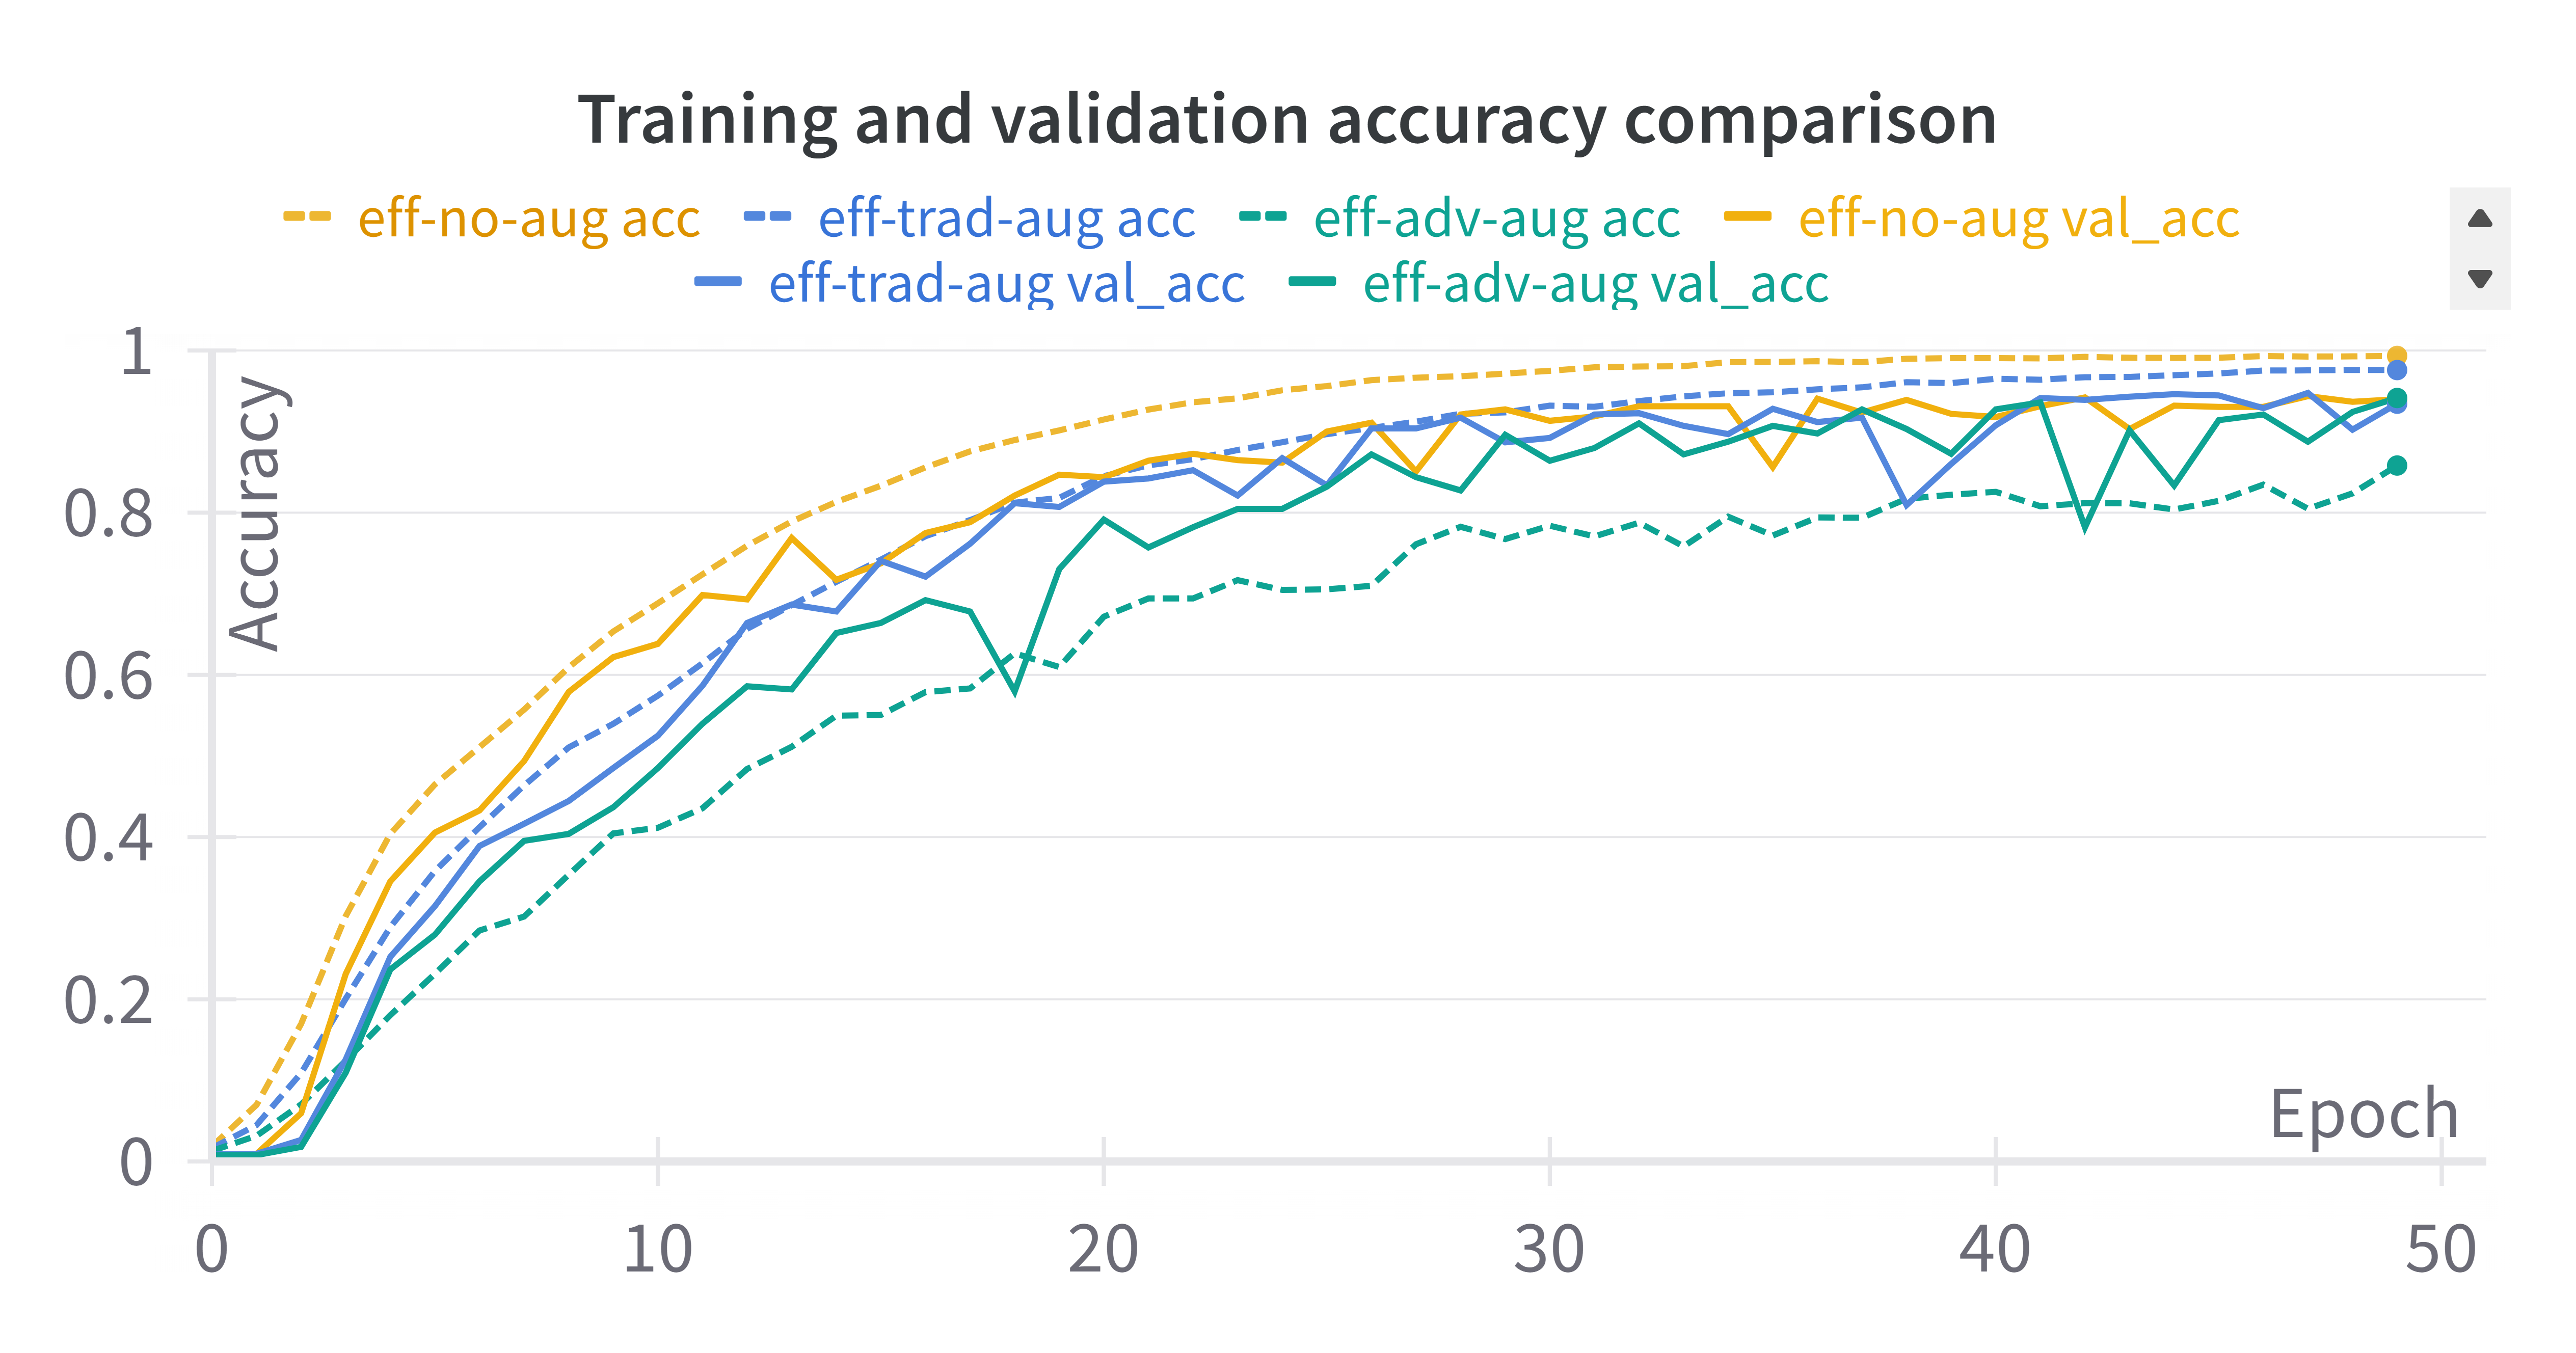
\includegraphics[width=0.95\textwidth]{Images/flowers-results/efficientNetLC.png}
    \caption{\textit{EfficientNet} learning curves.}
    \label{fig:efficientLC}
\end{figure}


The plot illustrates the training (dashed line) and validation (solid line) accuracy of models utilizing different data augmentation techniques over $50$ epochs. The yellow lines represent the model without data augmentation, the blue lines correspond to the model with traditional data augmentation, and the green lines depict the model with advanced data augmentation.

The model without data augmentation achieves the highest training accuracy, consistently increasing and achieving almost 100\% by the end of the $50$ epochs. The model with advanced data augmentation has the lowest training accuracy among the three. This might suggest that the advanced augmentation makes the training process more challenging, potentially leading to a more robust and generalized model.

Interestingly, despite the differences in training accuracy, the end validation accuracy for all three models is almost the same. This suggests that, regardless of the augmentation technique used, the models converge to a comparable level of performance on the validation set. \textit{EfficientNet's} performance is better than \textit{ResNet's} performance without data augmentation, but worse than \textit{ResNet's} performance with data augmentation applied. Table \ref{tab:effTable} shows a comparison of the \textit{EfficientNet} metrics for the best epoch. The model trained on the dataset augmented using advanced techniques performed slightly worse on the validation set than the model trained without data augmentation but handles the test set as good as the best model trained on the traditionally augmented dataset. 

\begin{table}[h!]
\centering
\caption{EfficientNet metrics comparison.}
\begin{tabular}{| >{\centering\arraybackslash}m{2.5cm} !{\vrule width 1.5pt} >{\centering\arraybackslash}m{1.0cm} | >{\centering\arraybackslash}m{1.0cm} !{\vrule width 1.5pt} >{\centering\arraybackslash}m{1.0cm} | >{\centering\arraybackslash}m{1.0cm} !{\vrule width 1.5pt} >{\centering\arraybackslash}m{1.0cm} | >{\centering\arraybackslash}m{1.0cm} !{\vrule width 1.5pt} >{\centering\arraybackslash}m{1.0cm}|}
\hline
\multirow{2}{*}{\textbf{Augmentation}} & \multicolumn{2}{c!{\vrule width 1.5pt}}{\textbf{Train}} & \multicolumn{2}{c!{\vrule width 1.5pt}}{\textbf{Val}} & \multicolumn{2}{c!{\vrule width 1.5pt}}{\textbf{Test}} \\
\cline{2-7}
 & \textbf{Acc} & \textbf{AUC} & \textbf{Acc} & \textbf{AUC} & \textbf{Acc} & \textbf{F1} \\
\hline
no-aug & 99.25 & 99.99 & 94.38 & 98.12 & 94.08 & 93.80 \\
\hline
trad-aug & 97.55 & 99.65 & 94.77 & 98.47 & 94.81 & 94.53 \\
\hline
adv-aug & 85.81 & 56.66 & 94.14 & 98.25 & 94.81 & 94.49 \\
\hline
\end{tabular}
\label{tab:effTable}
\end{table}

The plot in Figure \ref{fig:effResLC} compares the training accuracy of \textit{EfficientNet} and \textit{ResNet} models \textbf{without data augmentation} over $35$ epochs. The yellow line represents the training accuracy of the \textit{EfficientNet} model, while the purple line represents the training accuracy of the \textit{ResNet} model. 

\begin{figure}[!h]
    \centering
    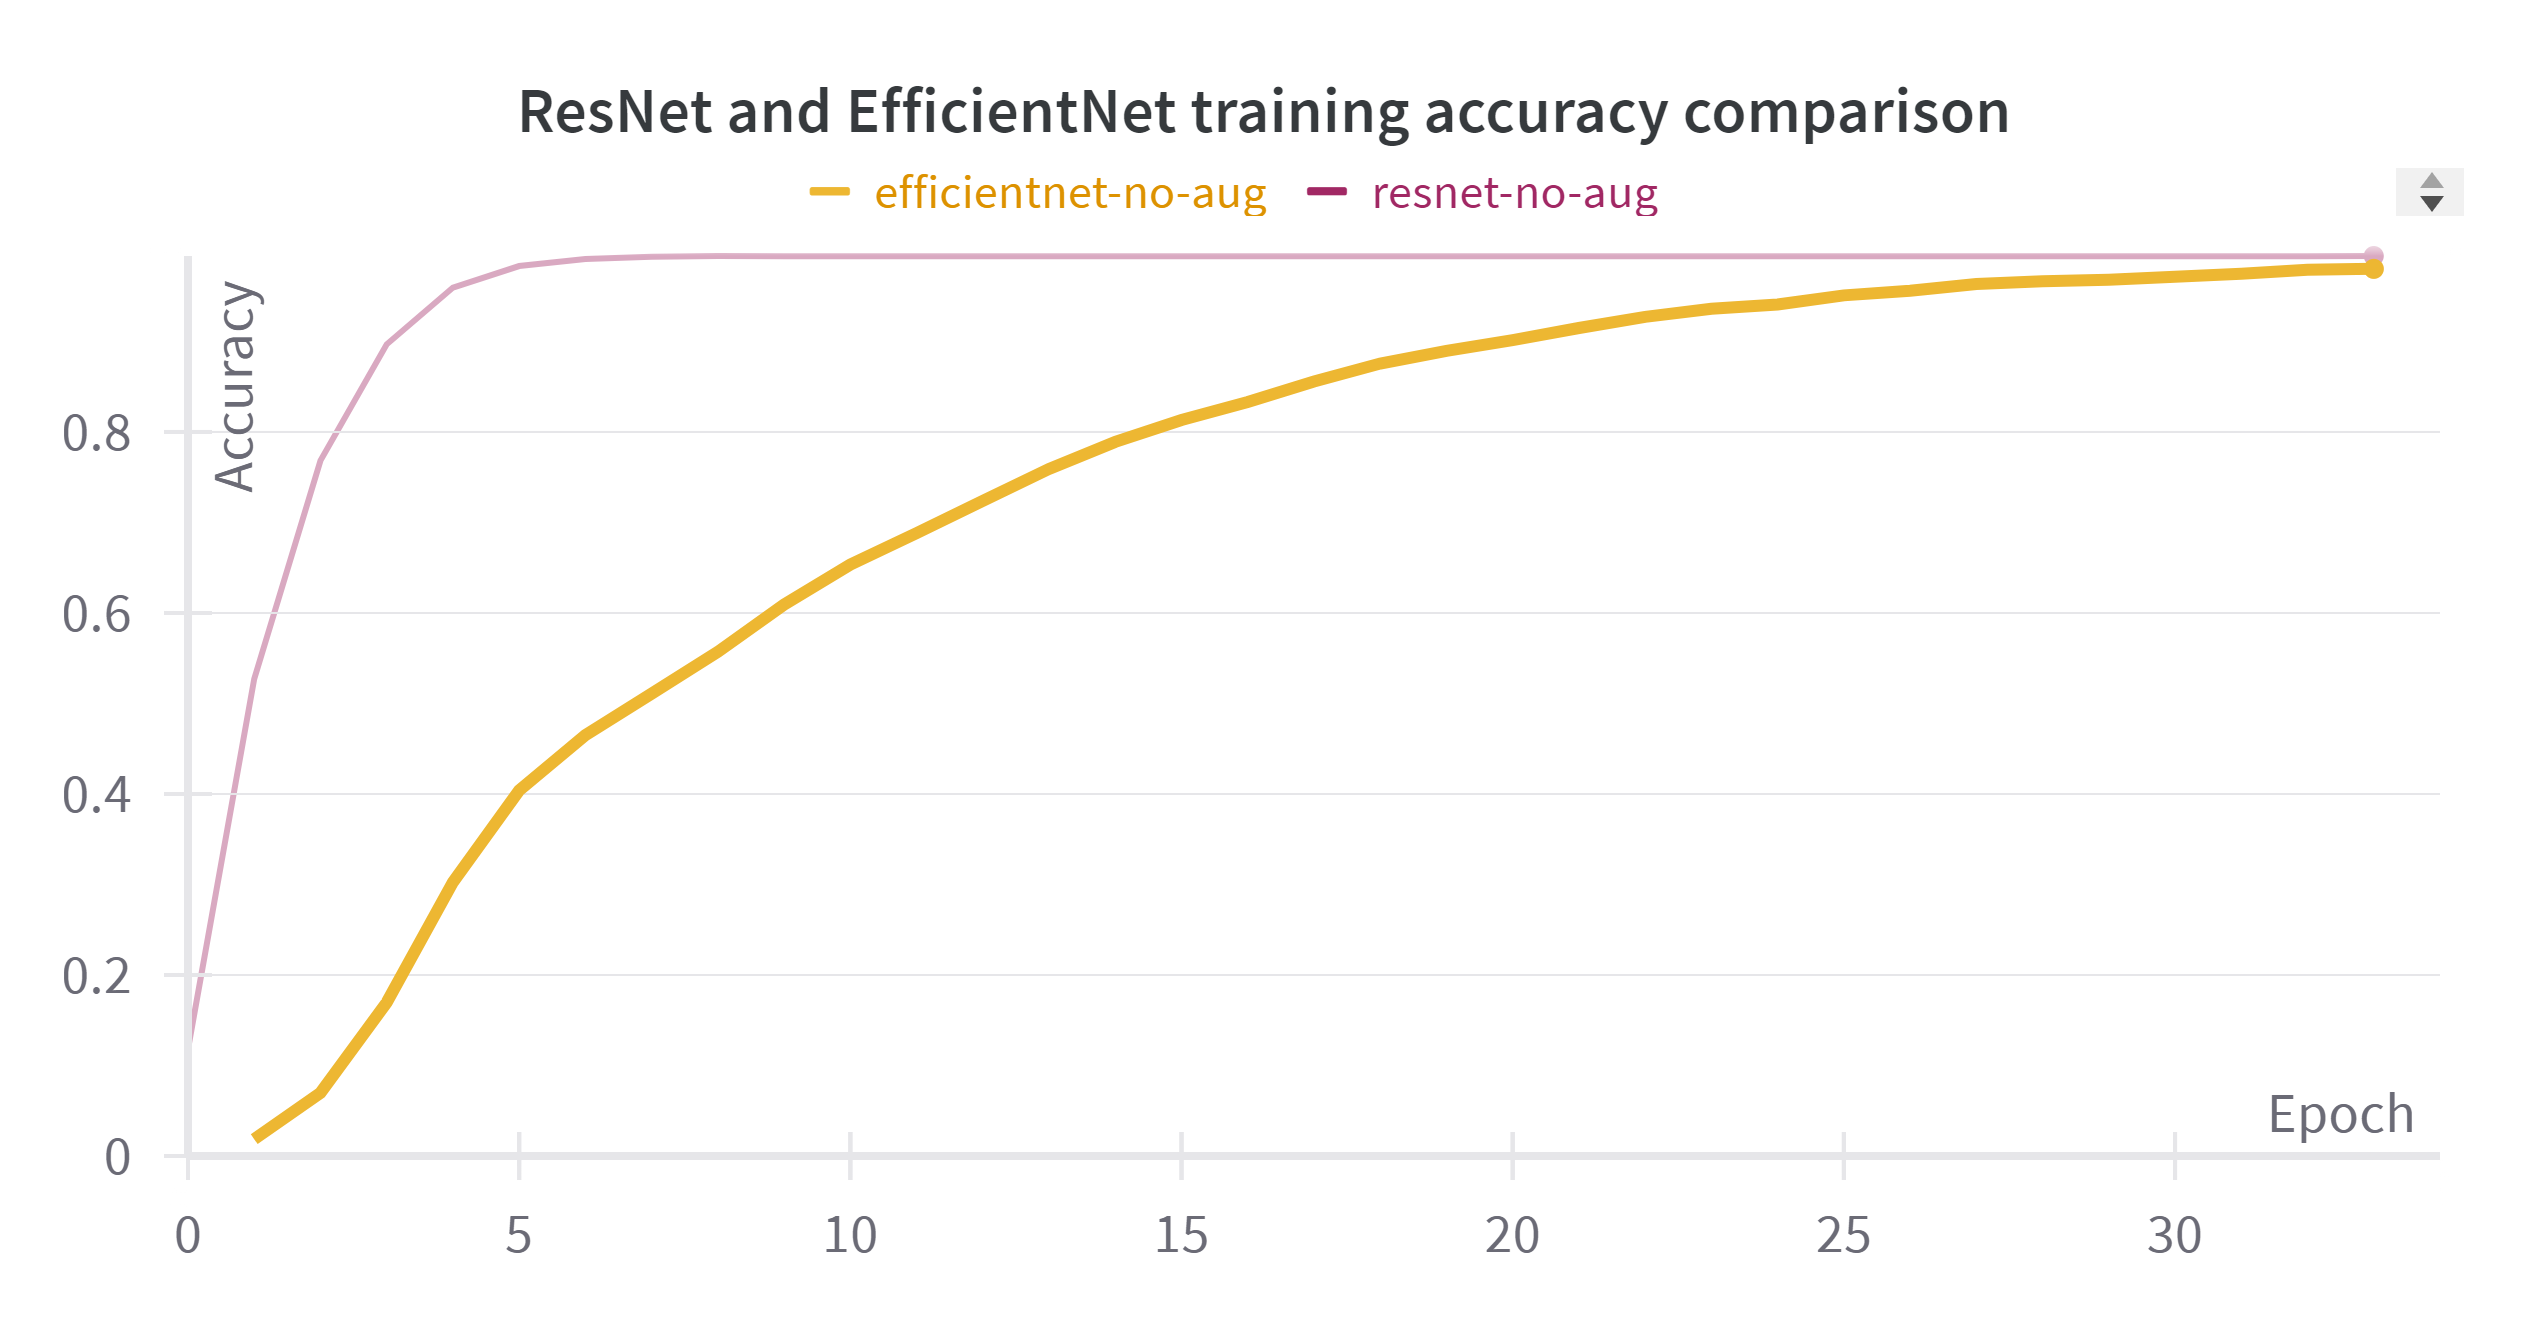
\includegraphics[width=0.95\textwidth]{Images/flowers-results/efficient-resnet-no-aug-lc.png}
    \caption{EfficientNet and ResNet learning curves without data augmentation.}
    \label{fig:effResLC}
\end{figure}

The \textit{ResNet} model converges much faster than the \textit{EfficientNet} model, achieving 98\% of the training accuracy after only $5$ epochs and stabilizing earlier. It means that the \textit{ResNet} model overfits the training data having more parameters than the \textit{EfficientNet} model while \textit{EfficientNet} keeps learning throughout all the epochs. This observation aligns with previous experiments showing that \textit{EfficientNet-B0}, with its $4$ million parameters, does not benefit from data augmentation as much as \textit{ResNet}, which has $20$ million parameters. The larger capacity of \textit{ResNet} allows it to leverage augmented data more effectively, improving its performance significantly. \textit{EfficientNet}, being a more parameter-efficient model, shows less pronounced benefits from data augmentation, suggesting it relies more on its architectural efficiency and less on extensive data augmentation for high accuracy.

\begin{figure}[!h]
    \centering
    \begin{subfigure}[b]{0.65\textwidth}
        \centering
        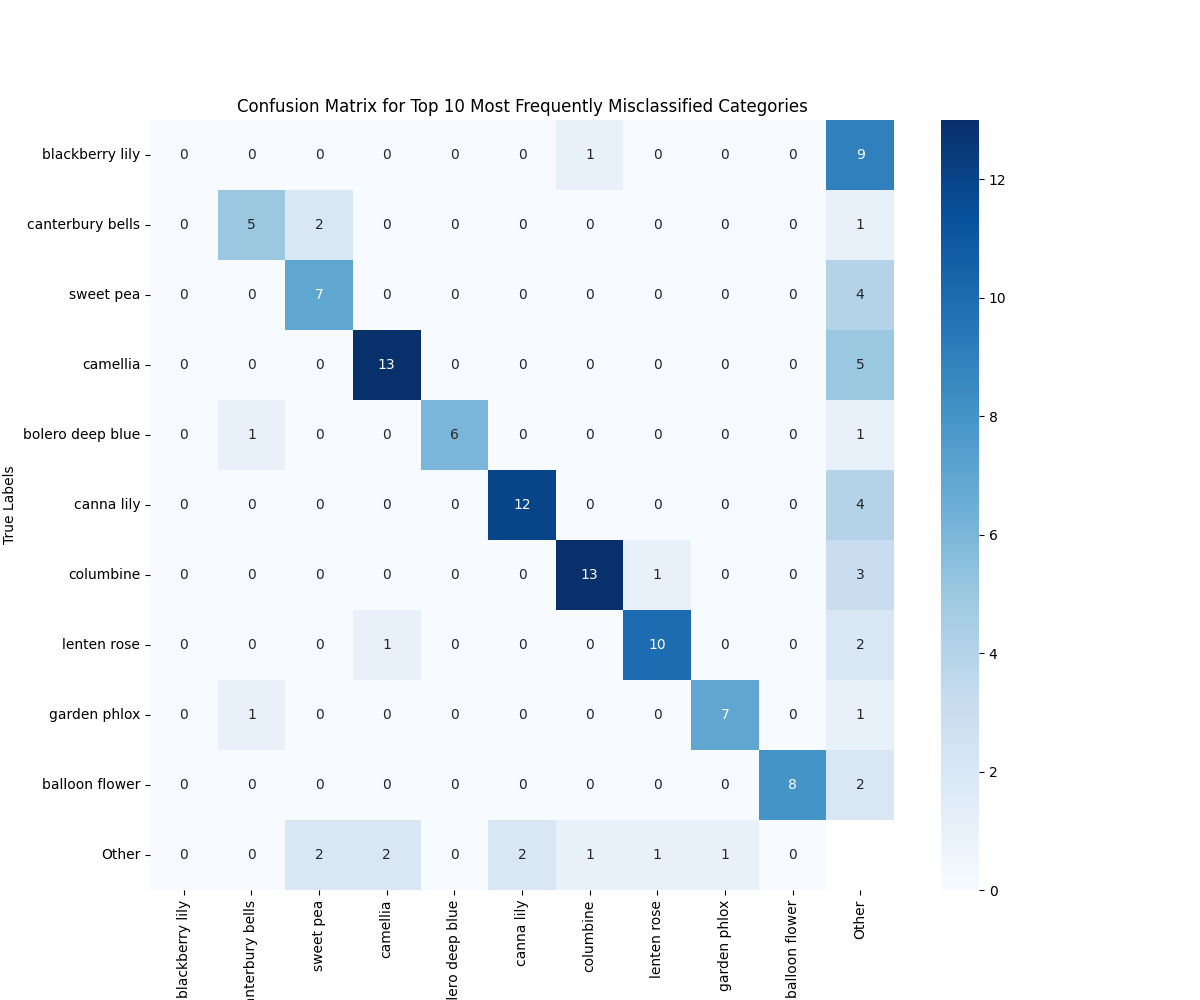
\includegraphics[width=\textwidth]{Images/flowers-results/confusion_matrix_no_aug.png}
        \caption{Without augmentation}
    \end{subfigure}

    \begin{subfigure}[b]{0.65\textwidth}
        \centering
        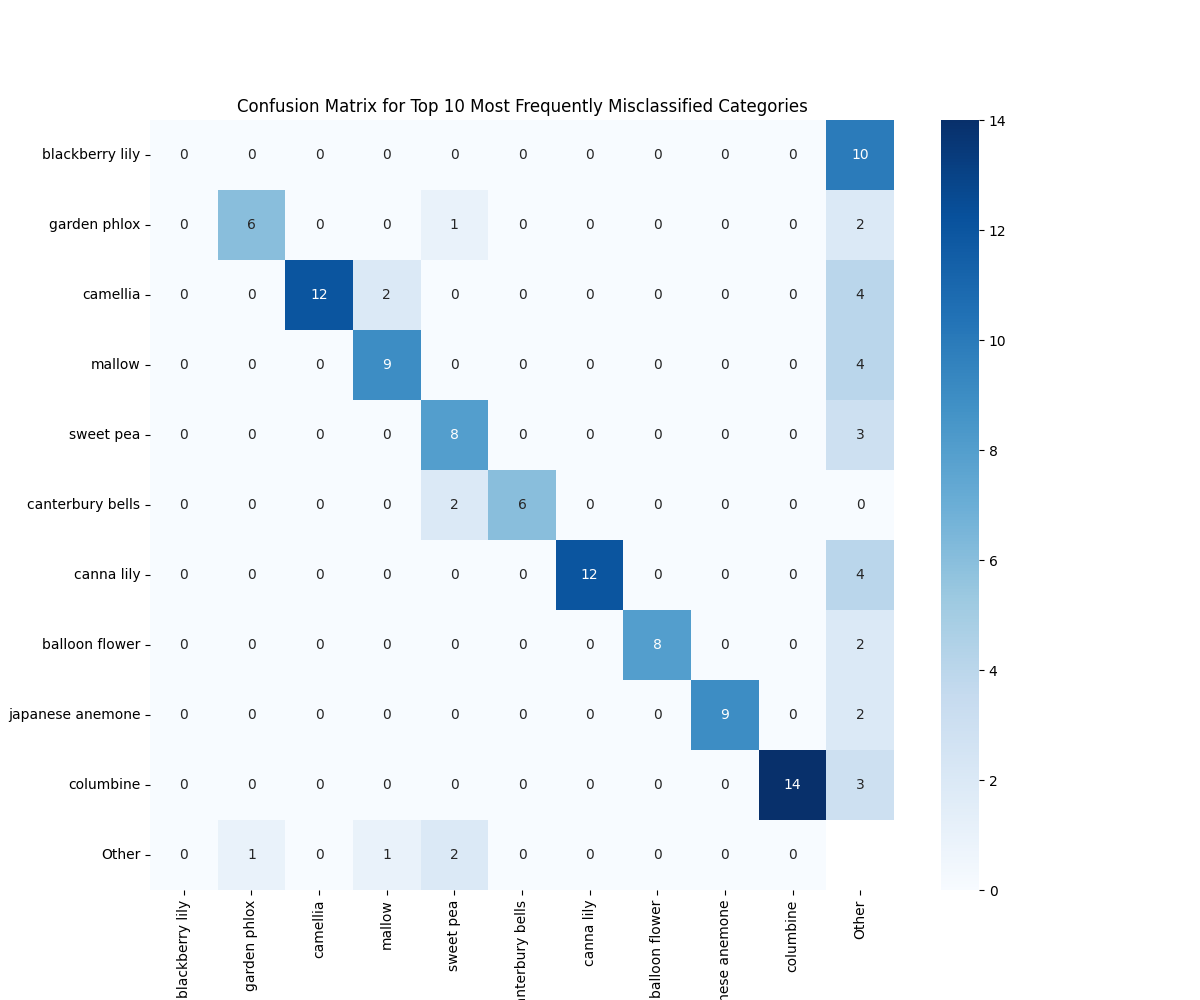
\includegraphics[width=\textwidth]{Images/flowers-results/confusion_matrix_adv_aug.png}
        \caption{With advanced augmentation}
    \end{subfigure}
    \caption{Confusion matrices for the top 10 worst-performing species of flowers.}
    \label{fig:confMatricesFlowersEfficient}
\end{figure}

Because Flowers dataset contains $102$ classes, plotting the complete confusion matrix is not practical. Figure \ref{fig:confMatricesFlowersEfficient} shows \textbf{confusion matrices} for the top $10$ worst-performing flower species before and after data augmentation. These species were selected based on the proportion of misclassified samples. 


The confusion matrices reveal that while data augmentation slightly improves the results for most of these worst-performing species, it does not affect the classification of the \textit{blackberry lily}, which remains entirely misclassified in both models.

For the final comparison, saliency maps were used to examine what the model focuses on with and without augmentation. These evaluations were done manually, and the implications of the findings are summarized below.

In most cases, both networks focus on similar areas of the input image, as shown in Figure \ref{fig:saliency1}. This is expected since the accuracy of the models is not much different.

\begin{figure}[h!]
    \centering
    \begin{subfigure}[b]{0.32\textwidth}
        \centering
        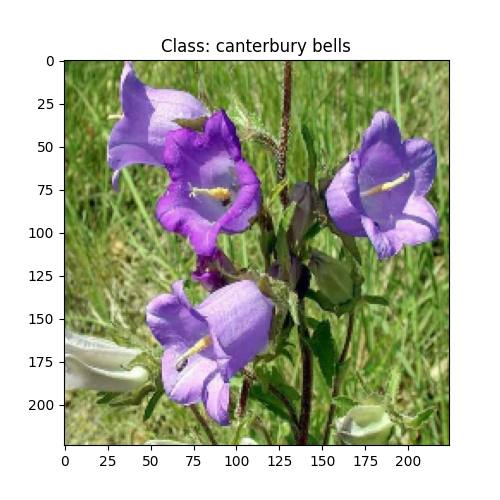
\includegraphics[width=\textwidth]{Images/saliency-flowers/510/image_510.png}
        \caption{Preprocessed image}
    \end{subfigure}
    \hfill
    \begin{subfigure}[b]{0.32\textwidth}
        \centering
        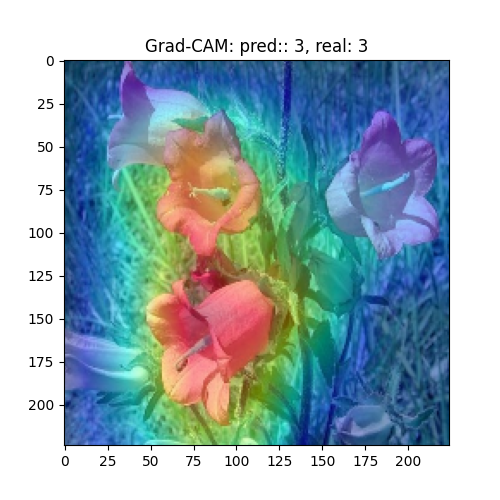
\includegraphics[width=\textwidth]{Images/saliency-flowers/510/GradCAM_510_no_aug.png}
        \caption{Without augmentation}
    \end{subfigure}
    \hfill
    \begin{subfigure}[b]{0.32\textwidth}
        \centering
        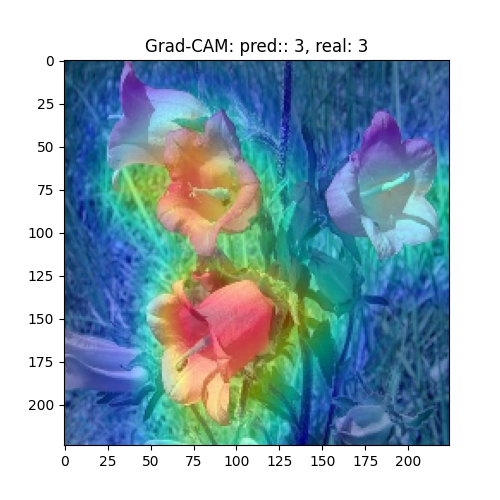
\includegraphics[width=\textwidth]{Images/saliency-flowers/510/GradCAM_510_aug.png}
        \caption{With augmentation}
    \end{subfigure}
    \caption{Similar saliency maps with and without augmentation.}
    \label{fig:saliency1}
\end{figure}

The biggest difference appears when a model trained without data augmentation makes mistakes that a model trained with augmented data avoids. Figure \ref{fig:saliency2} shows this with a \textit{lotus} flower example. The saliency map for the first model, trained without augmentation highlights the yellow stamen of the flower, causing confusion with the \textit{columbine} flower, which also has prominent yellow parts. In contrast, the model trained on augmented data focused on the leaves and correctly classified the example.

\begin{figure}[h!]
    \centering
    \begin{subfigure}[b]{0.24\textwidth}
        \centering
        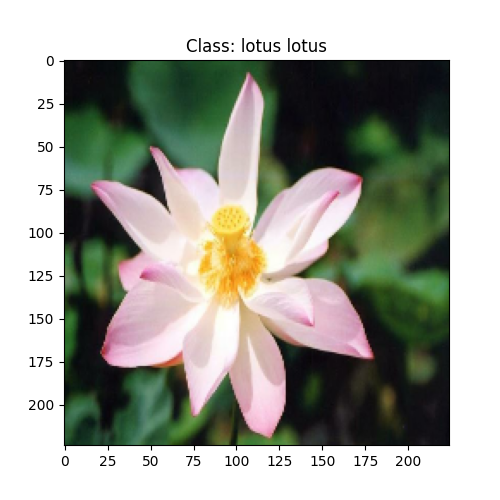
\includegraphics[width=\textwidth]{Images/saliency-flowers/172/image_172.png}
        \caption{Input image}
    \end{subfigure}
    \hfill
    \begin{subfigure}[b]{0.24\textwidth}
        \centering
        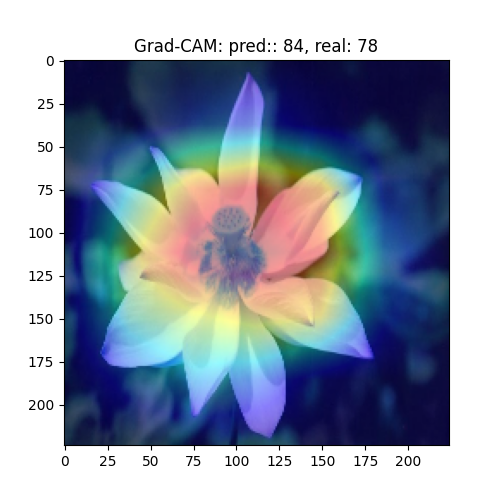
\includegraphics[width=\textwidth]{Images/saliency-flowers/172/GradCAM_no_aug.png}
        \caption{Without augmentation}
    \end{subfigure}
    \hfill
    \begin{subfigure}[b]{0.24\textwidth}
        \centering
        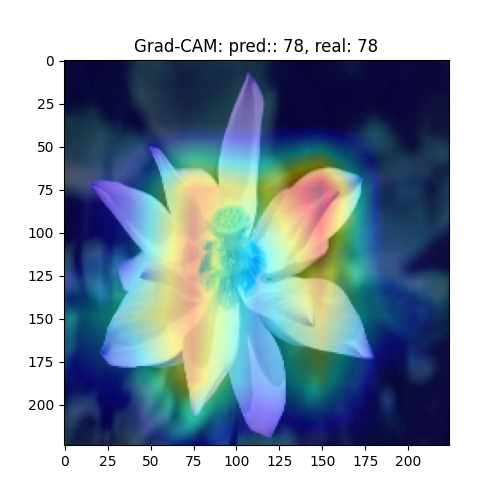
\includegraphics[width=\textwidth]{Images/saliency-flowers/172/GradCAM_172_aug.png}
        \caption{With augmentation}
    \end{subfigure}
    \hfill
    \begin{subfigure}[b]{0.24\textwidth}
        \centering
        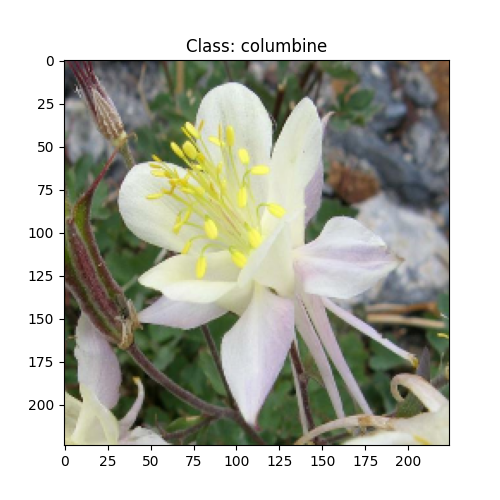
\includegraphics[width=\textwidth]{Images/saliency-flowers/172/image_320_wrong.png}
        \caption{Wrong prediction}
    \end{subfigure}
    \caption{Saliency maps for example misclassified by model trained without data augmentation.}
    \label{fig:saliency2}
\end{figure}

Using saliency maps, we can also visualize samples where data augmentation did not improve the prediction. As mentioned above, the confusion matrix revealed that \textit{blackberry lily} flowers are never correctly classified by any model. Analyzing images presented in Figure \ref{fig:saliency3} we can understand, that the model focused on the background instead of the flower. Augmentation methods which change the background of the image could improve the results.

\begin{figure}[h!]
    \centering
    \begin{subfigure}[b]{0.32\textwidth}
        \centering
        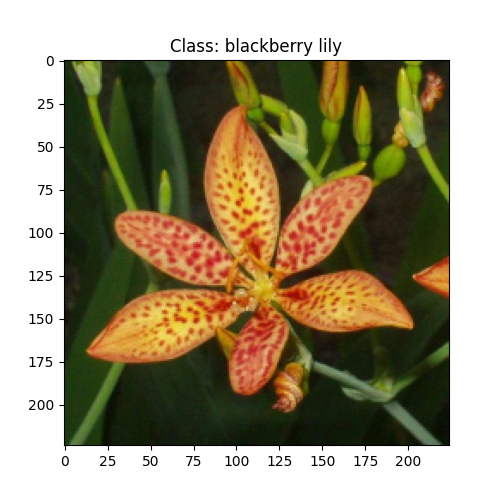
\includegraphics[width=\textwidth]{Images/saliency-flowers/249/image_249.png}
        \caption{Preprocessed image}
    \end{subfigure}
    \hfill
    \begin{subfigure}[b]{0.32\textwidth}
        \centering
        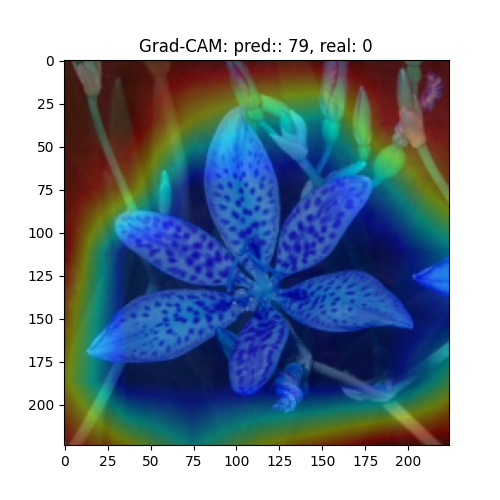
\includegraphics[width=\textwidth]{Images/saliency-flowers/249/GradCAM_249_no_aug.png}
        \caption{Without augmentation}
    \end{subfigure}
    \hfill
    \begin{subfigure}[b]{0.32\textwidth}
        \centering
        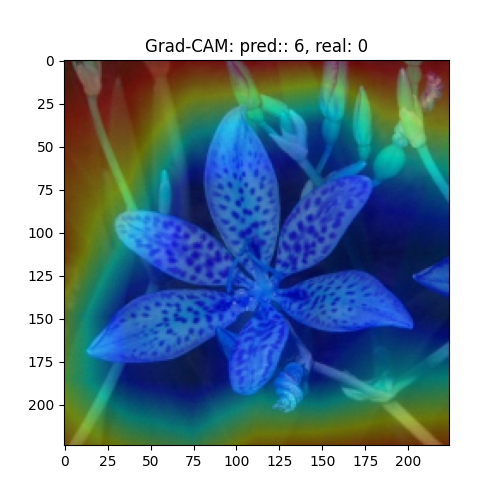
\includegraphics[width=\textwidth]{Images/saliency-flowers/249/GradCAM_249_aug.png}
        \caption{With augmentation}
    \end{subfigure}
    \caption{Saliency maps for class which performance did not improve thanks to data augmentation.}
    \label{fig:saliency3}
\end{figure}

The final experiment on this dataset involved over-augmenting the data. The batch of over-augmented data, with a 100\% probability of augmentation application, increased color contrast, and full rotations, is shown in Figure \ref{fig:overaug}. 

\begin{figure}[!h]
    \centering
    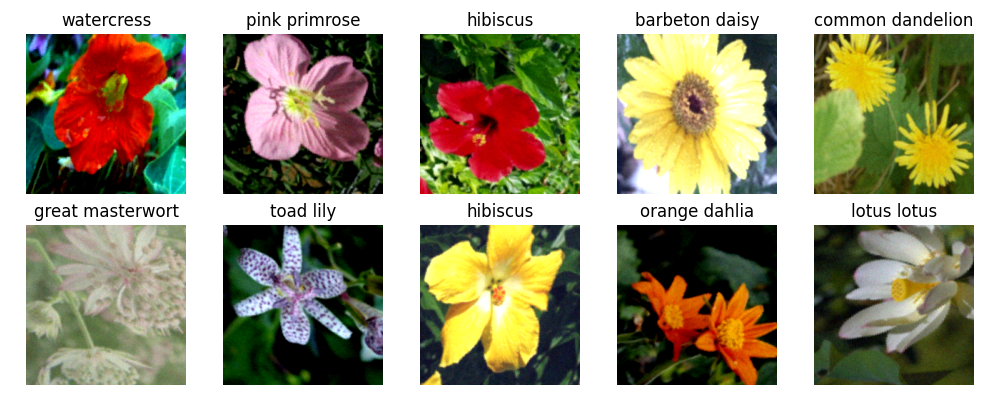
\includegraphics[width=0.9\textwidth]{Images/flowers-overaugmented/batch_overaugmented.png}
    \caption{Over-augmented batch.}
    \label{fig:overaug}
\end{figure}

Even though this batch does not appear over-augmented, the unnatural rotations and excessively high probability of application led to worse performance of the model trained on this augmented dataset compared to the unchanged dataset. These results are visible in Figure \ref{fig:overaugLC}. The validation accuracy of the model trained on the over-augmented dataset is around 83\%, which is \textbf{10 percentage points} less than the model trained without data augmentation. These results demonstrate that data augmentation does not always help and should be applied carefully.

\begin{figure}[!h]
    \centering
    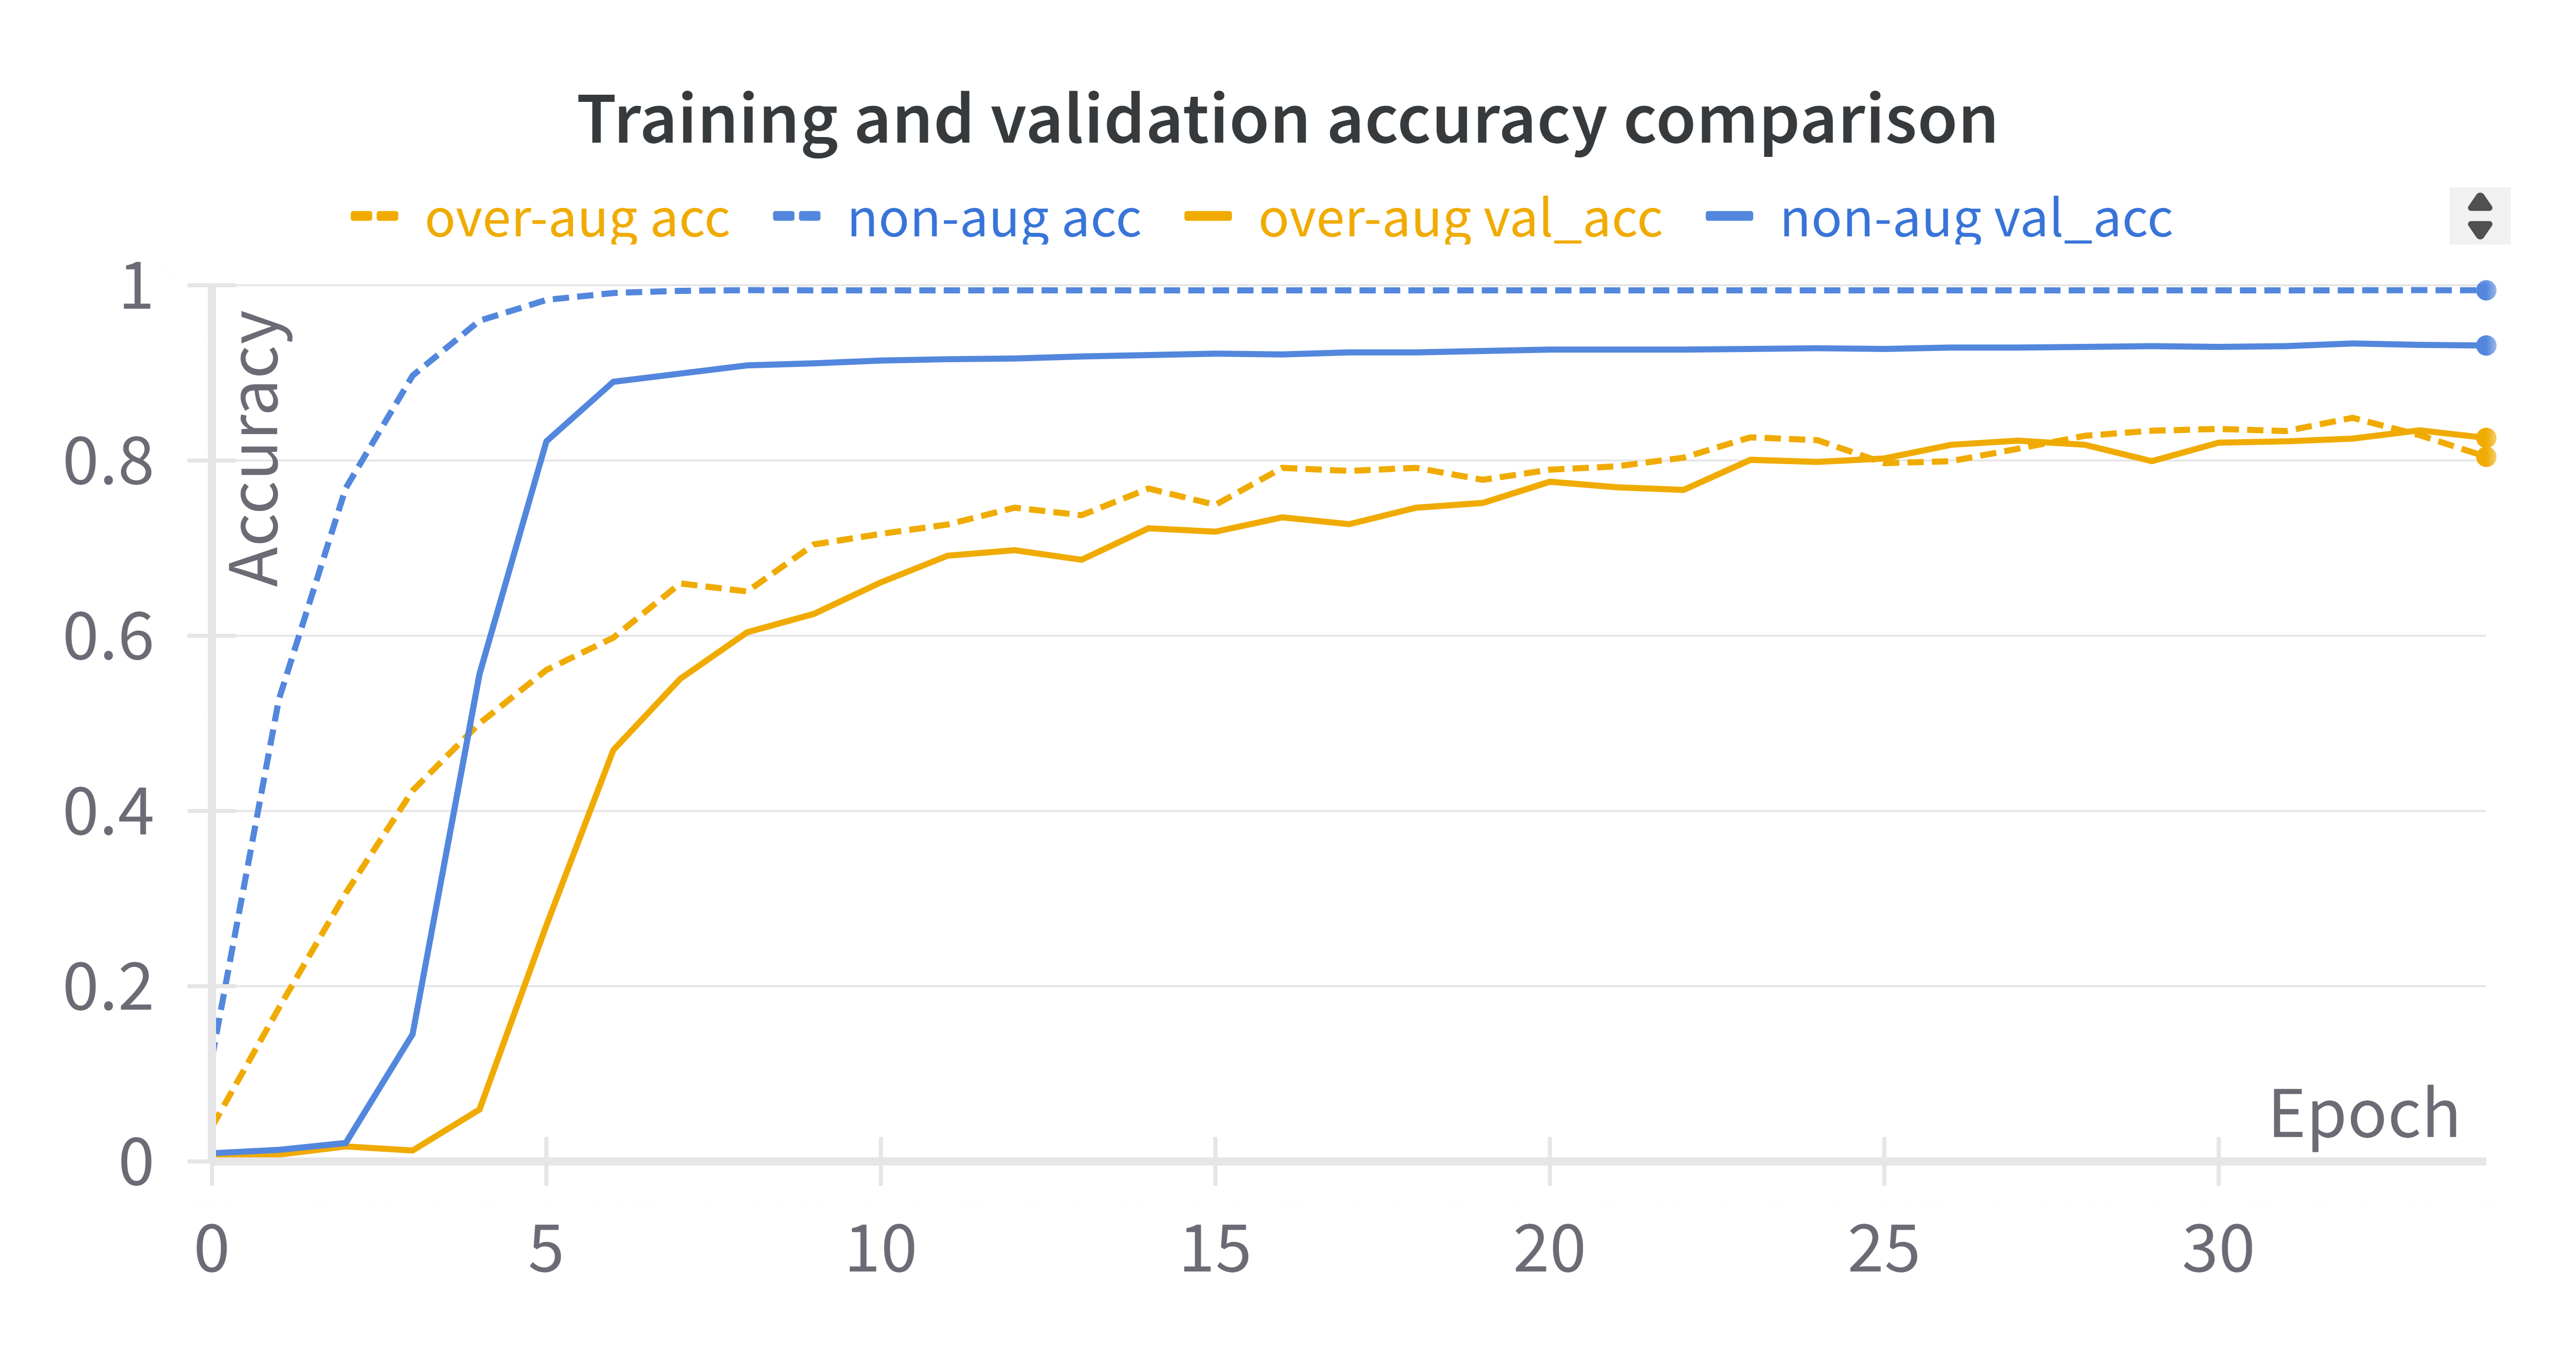
\includegraphics[width=0.95\textwidth]{Images/flowers-overaugmented/overaugLC.png}
    \caption{Comparison of learning curves for not augmented and over-augmented dataset.}
    \label{fig:overaugLC}
\end{figure}


\subsection{One-shot Flowers 102}
\label{ssec:resultsOneshotFlowers}

In this experiment, the number of flower samples was limited to $5$, $10$, and $20$ per class to evaluate the effectiveness of data augmentation under \textbf{limited data conditions}. If the number of examples in the original dataset was smaller than the threshold, examples were randomly repeated. This resulted in datasets of $510$, $1020$, and $2040$ samples, respectively, with 80\% used for training and 20\% for validation. Models were trained using $80$, $100$, and $120$ epochs to make stabilization of the training possible. The test set remained the same as in previous experiments ($1638$ examples).

Figures \ref{fig:oneshotLCsTrain} and \ref{fig:oneshotLCsVal} present training and validation learning curves of models trained on all the previously mentioned datasets. Each plot uses consistent colors: yellow represents the model trained on the dataset without data augmentation, orange indicates the use of \textit{MixUp} and \textit{CutMix} methods, blue is associated with traditional techniques, and green is utilized for advanced techniques that combine all the methods mentioned above.

\begin{figure}[!h]
    \centering
    \begin{subfigure}[b]{0.77\textwidth}
        \centering
        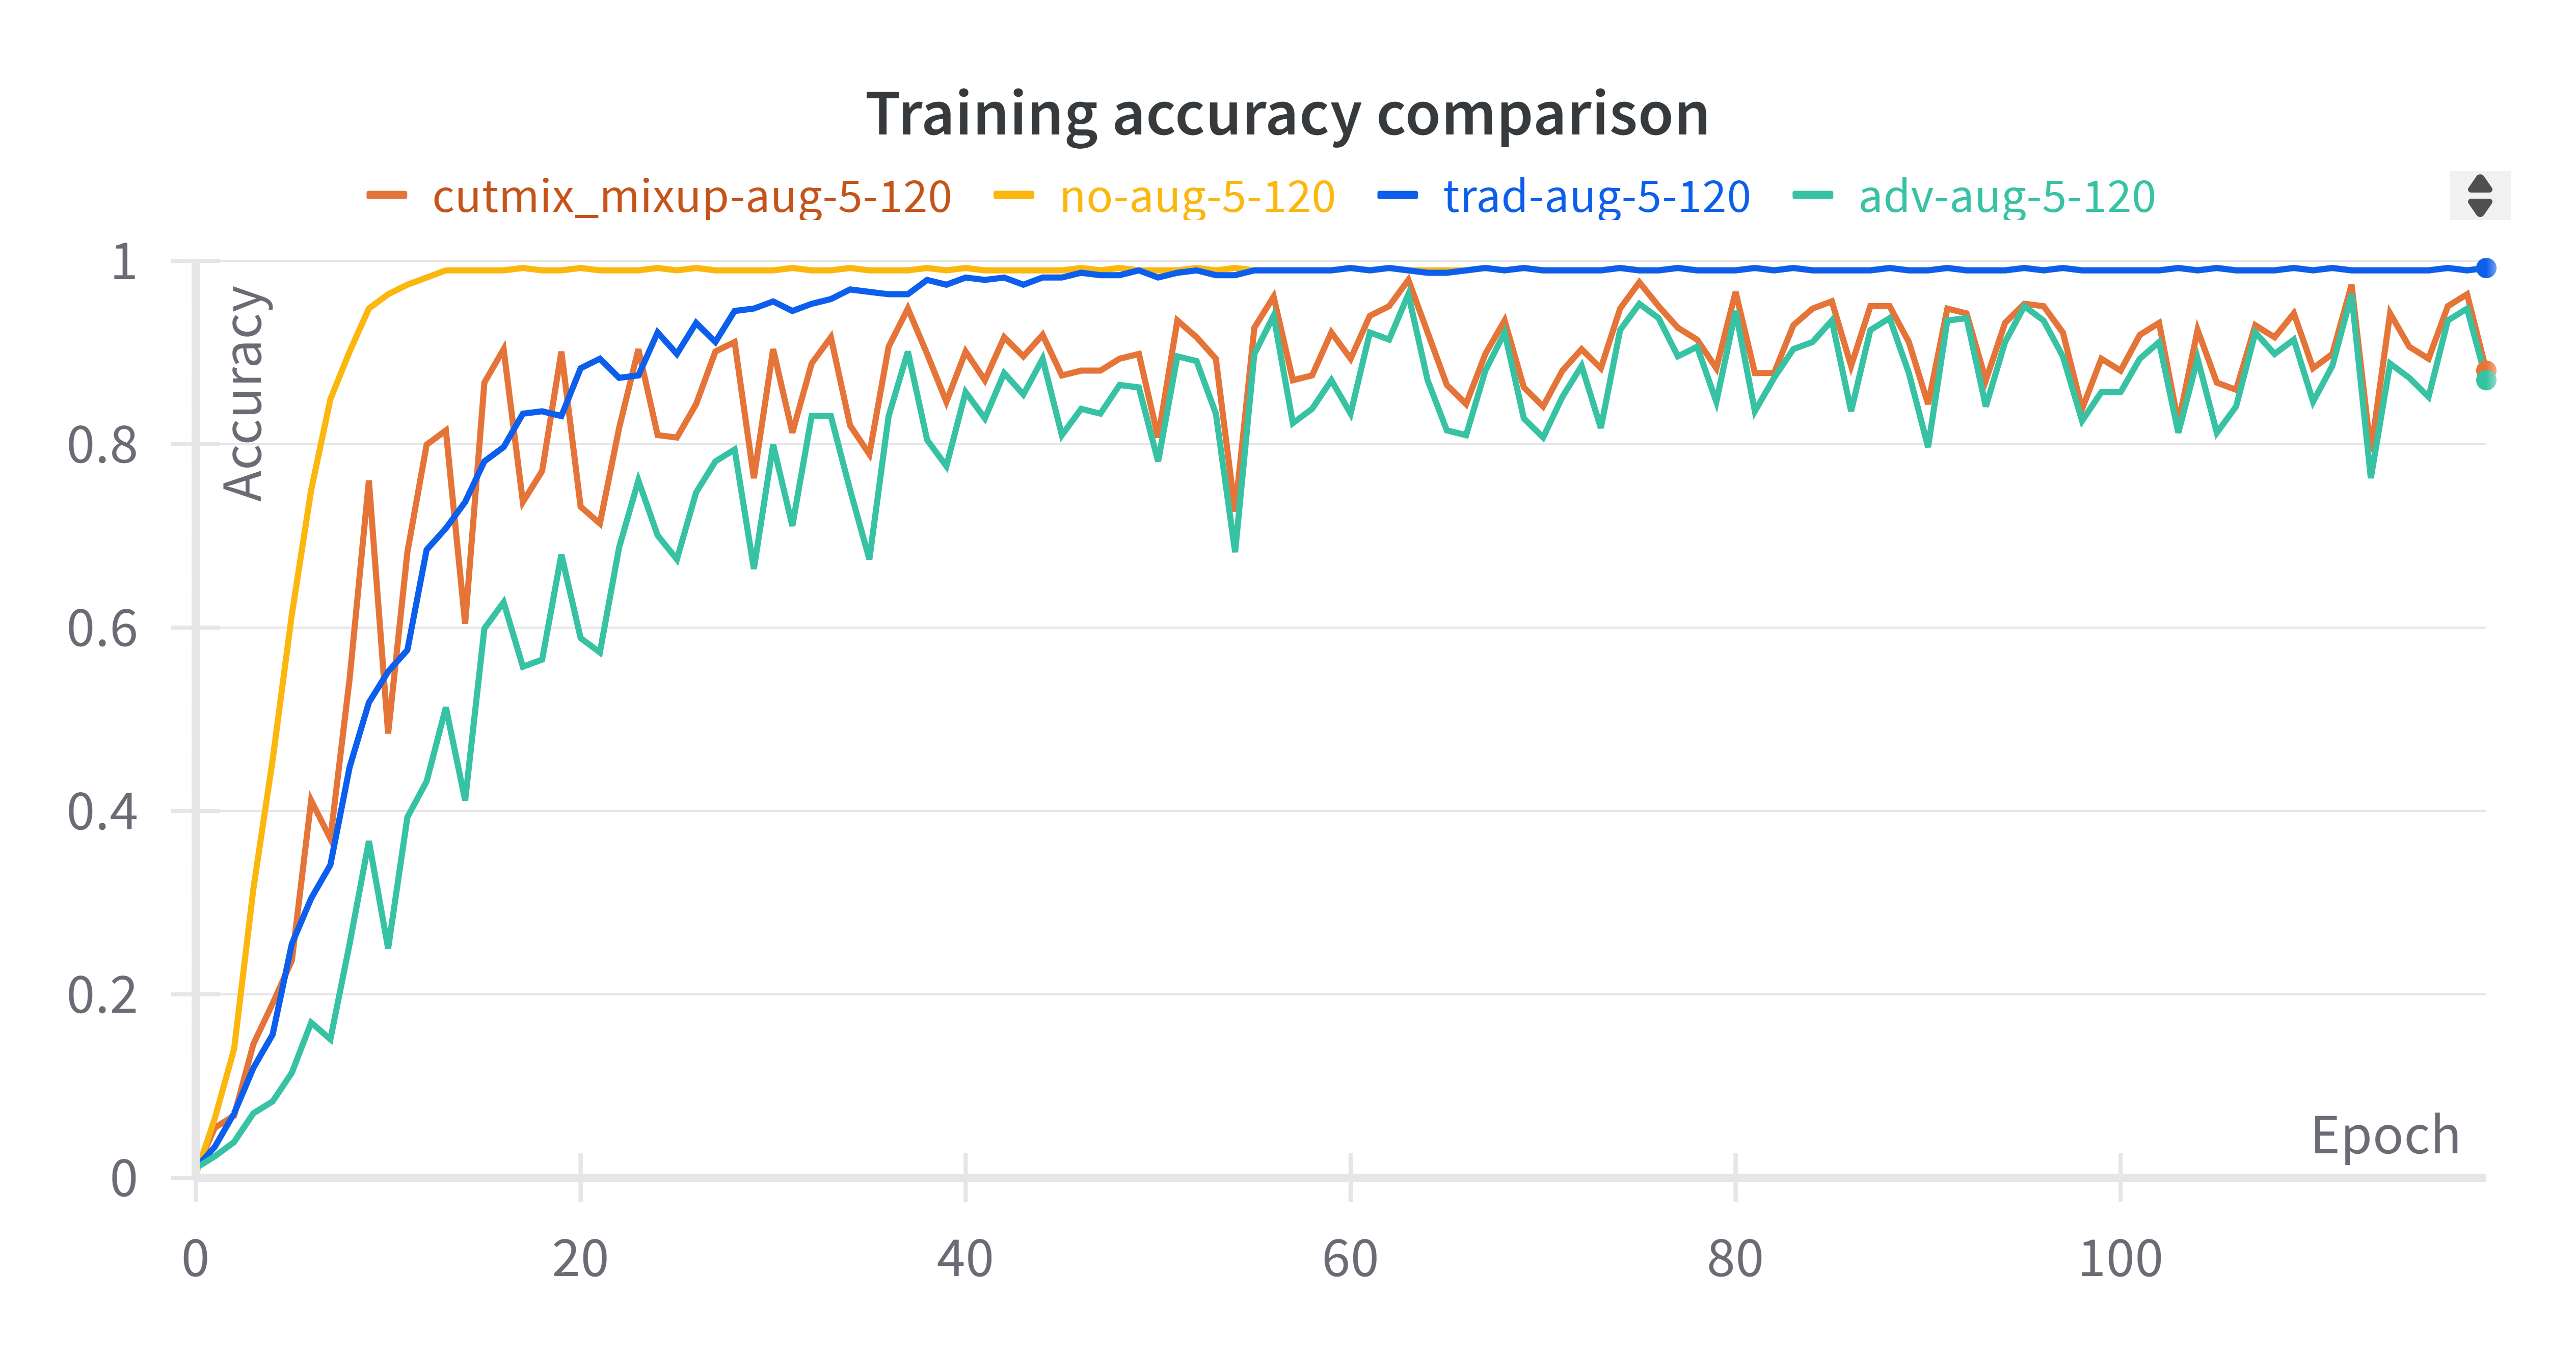
\includegraphics[width=\textwidth]{Images/oneshot/lc/train_acc_5.png}
        \caption{Training accuracy - 5 samples}
    \end{subfigure}

    \begin{subfigure}[b]{0.77\textwidth}
        \centering
        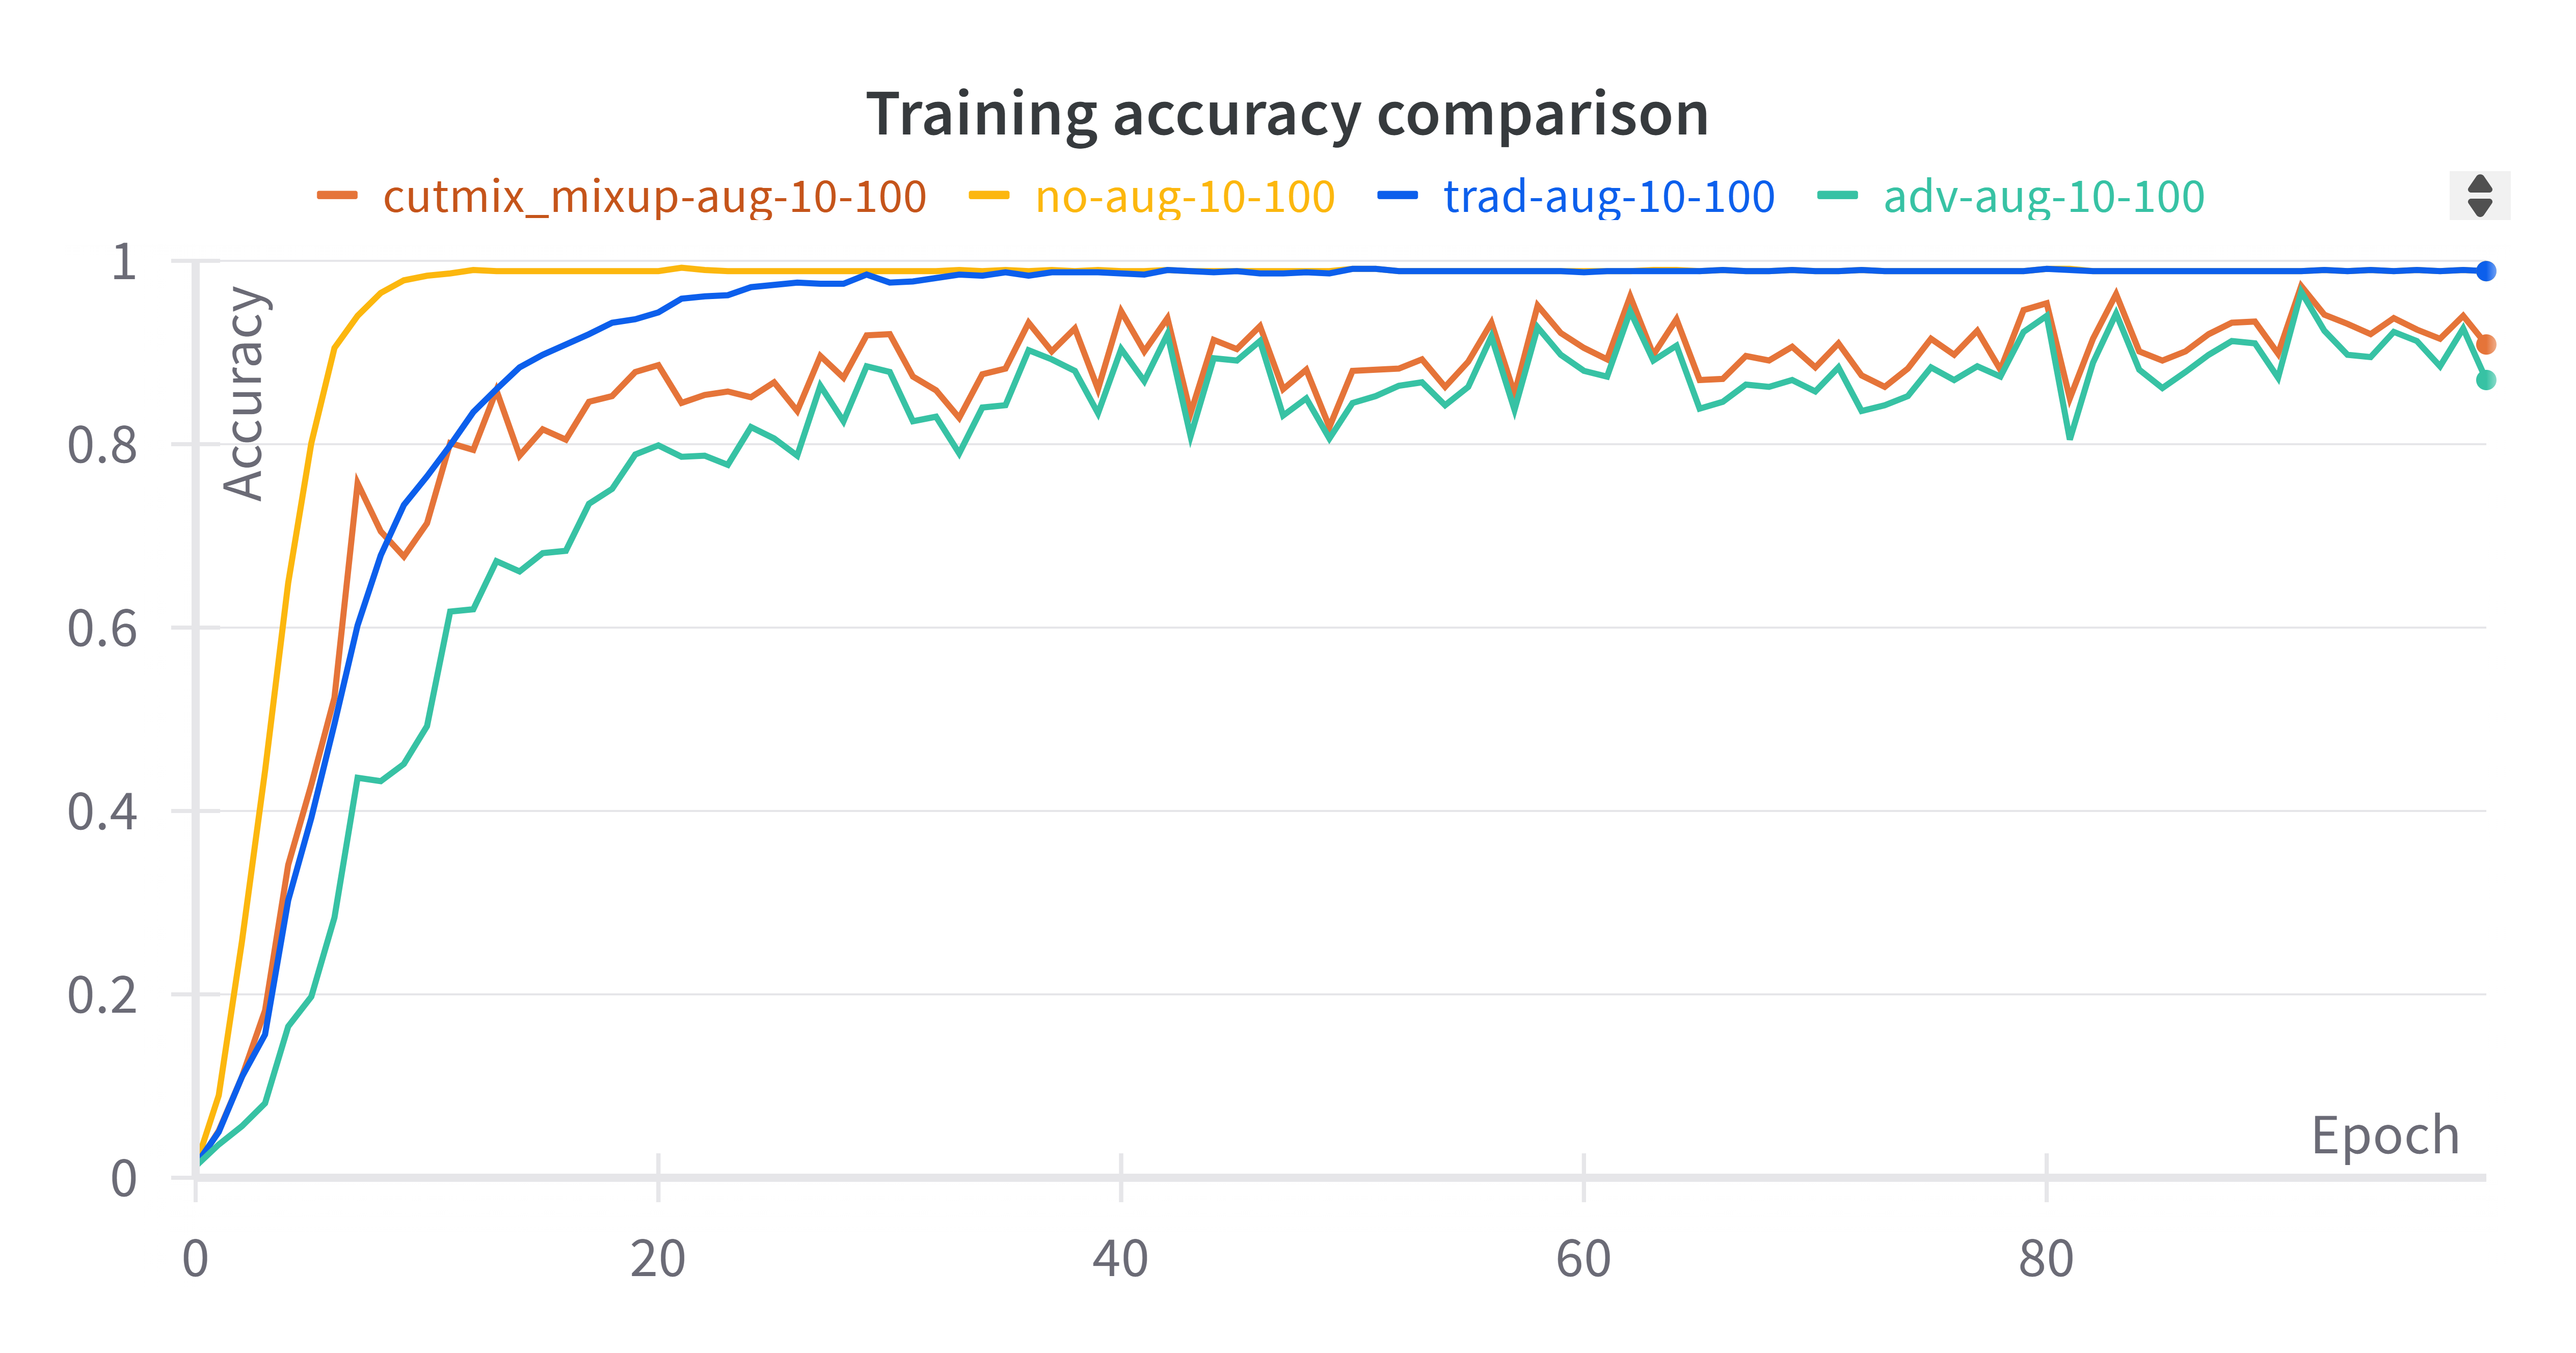
\includegraphics[width=\textwidth]{Images/oneshot/lc/train_acc_10.png}
        \caption{Training accuracy - 10 samples}
    \end{subfigure}


    \begin{subfigure}[b]{0.77\textwidth}
        \centering
        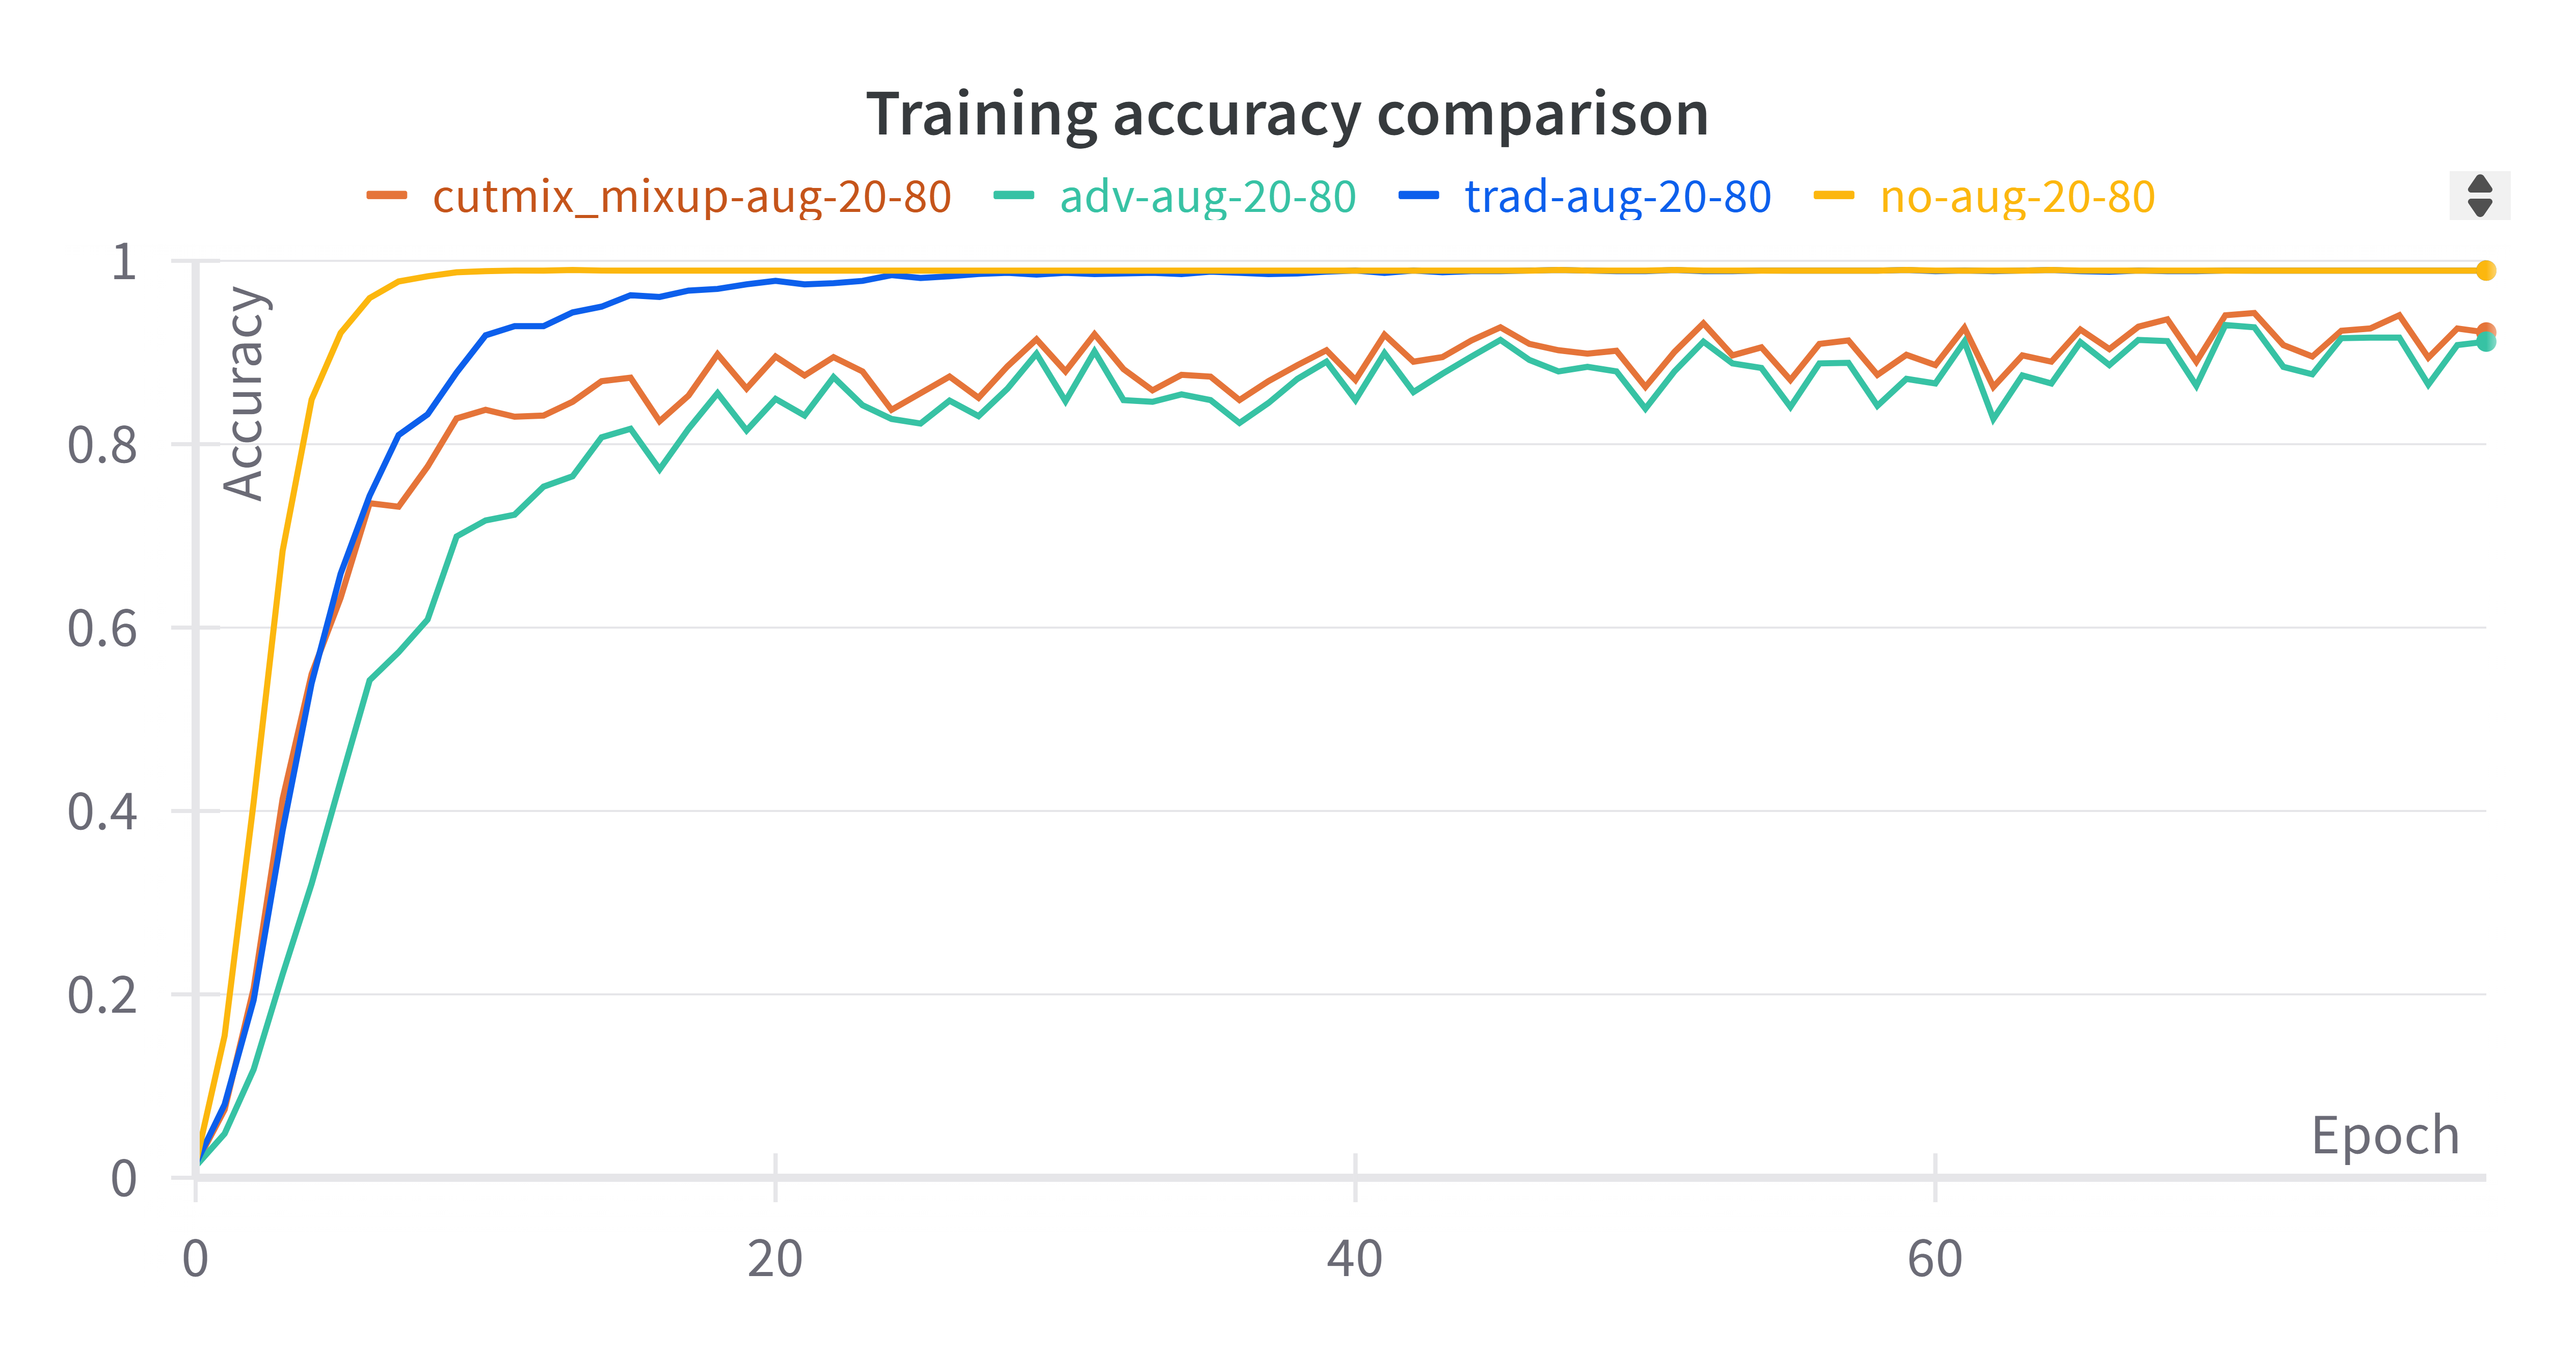
\includegraphics[width=\textwidth]{Images/oneshot/lc/train_acc_20.png}
        \caption{Training accuracy - 20 samples}
    \end{subfigure}

    \caption{Training learning curves for different sizes of Flowers 102 dataset.}
    \label{fig:oneshotLCsTrain}
   
\end{figure}

\begin{figure}[!h]
    \centering

    \begin{subfigure}[b]{0.77\textwidth}
        \centering
        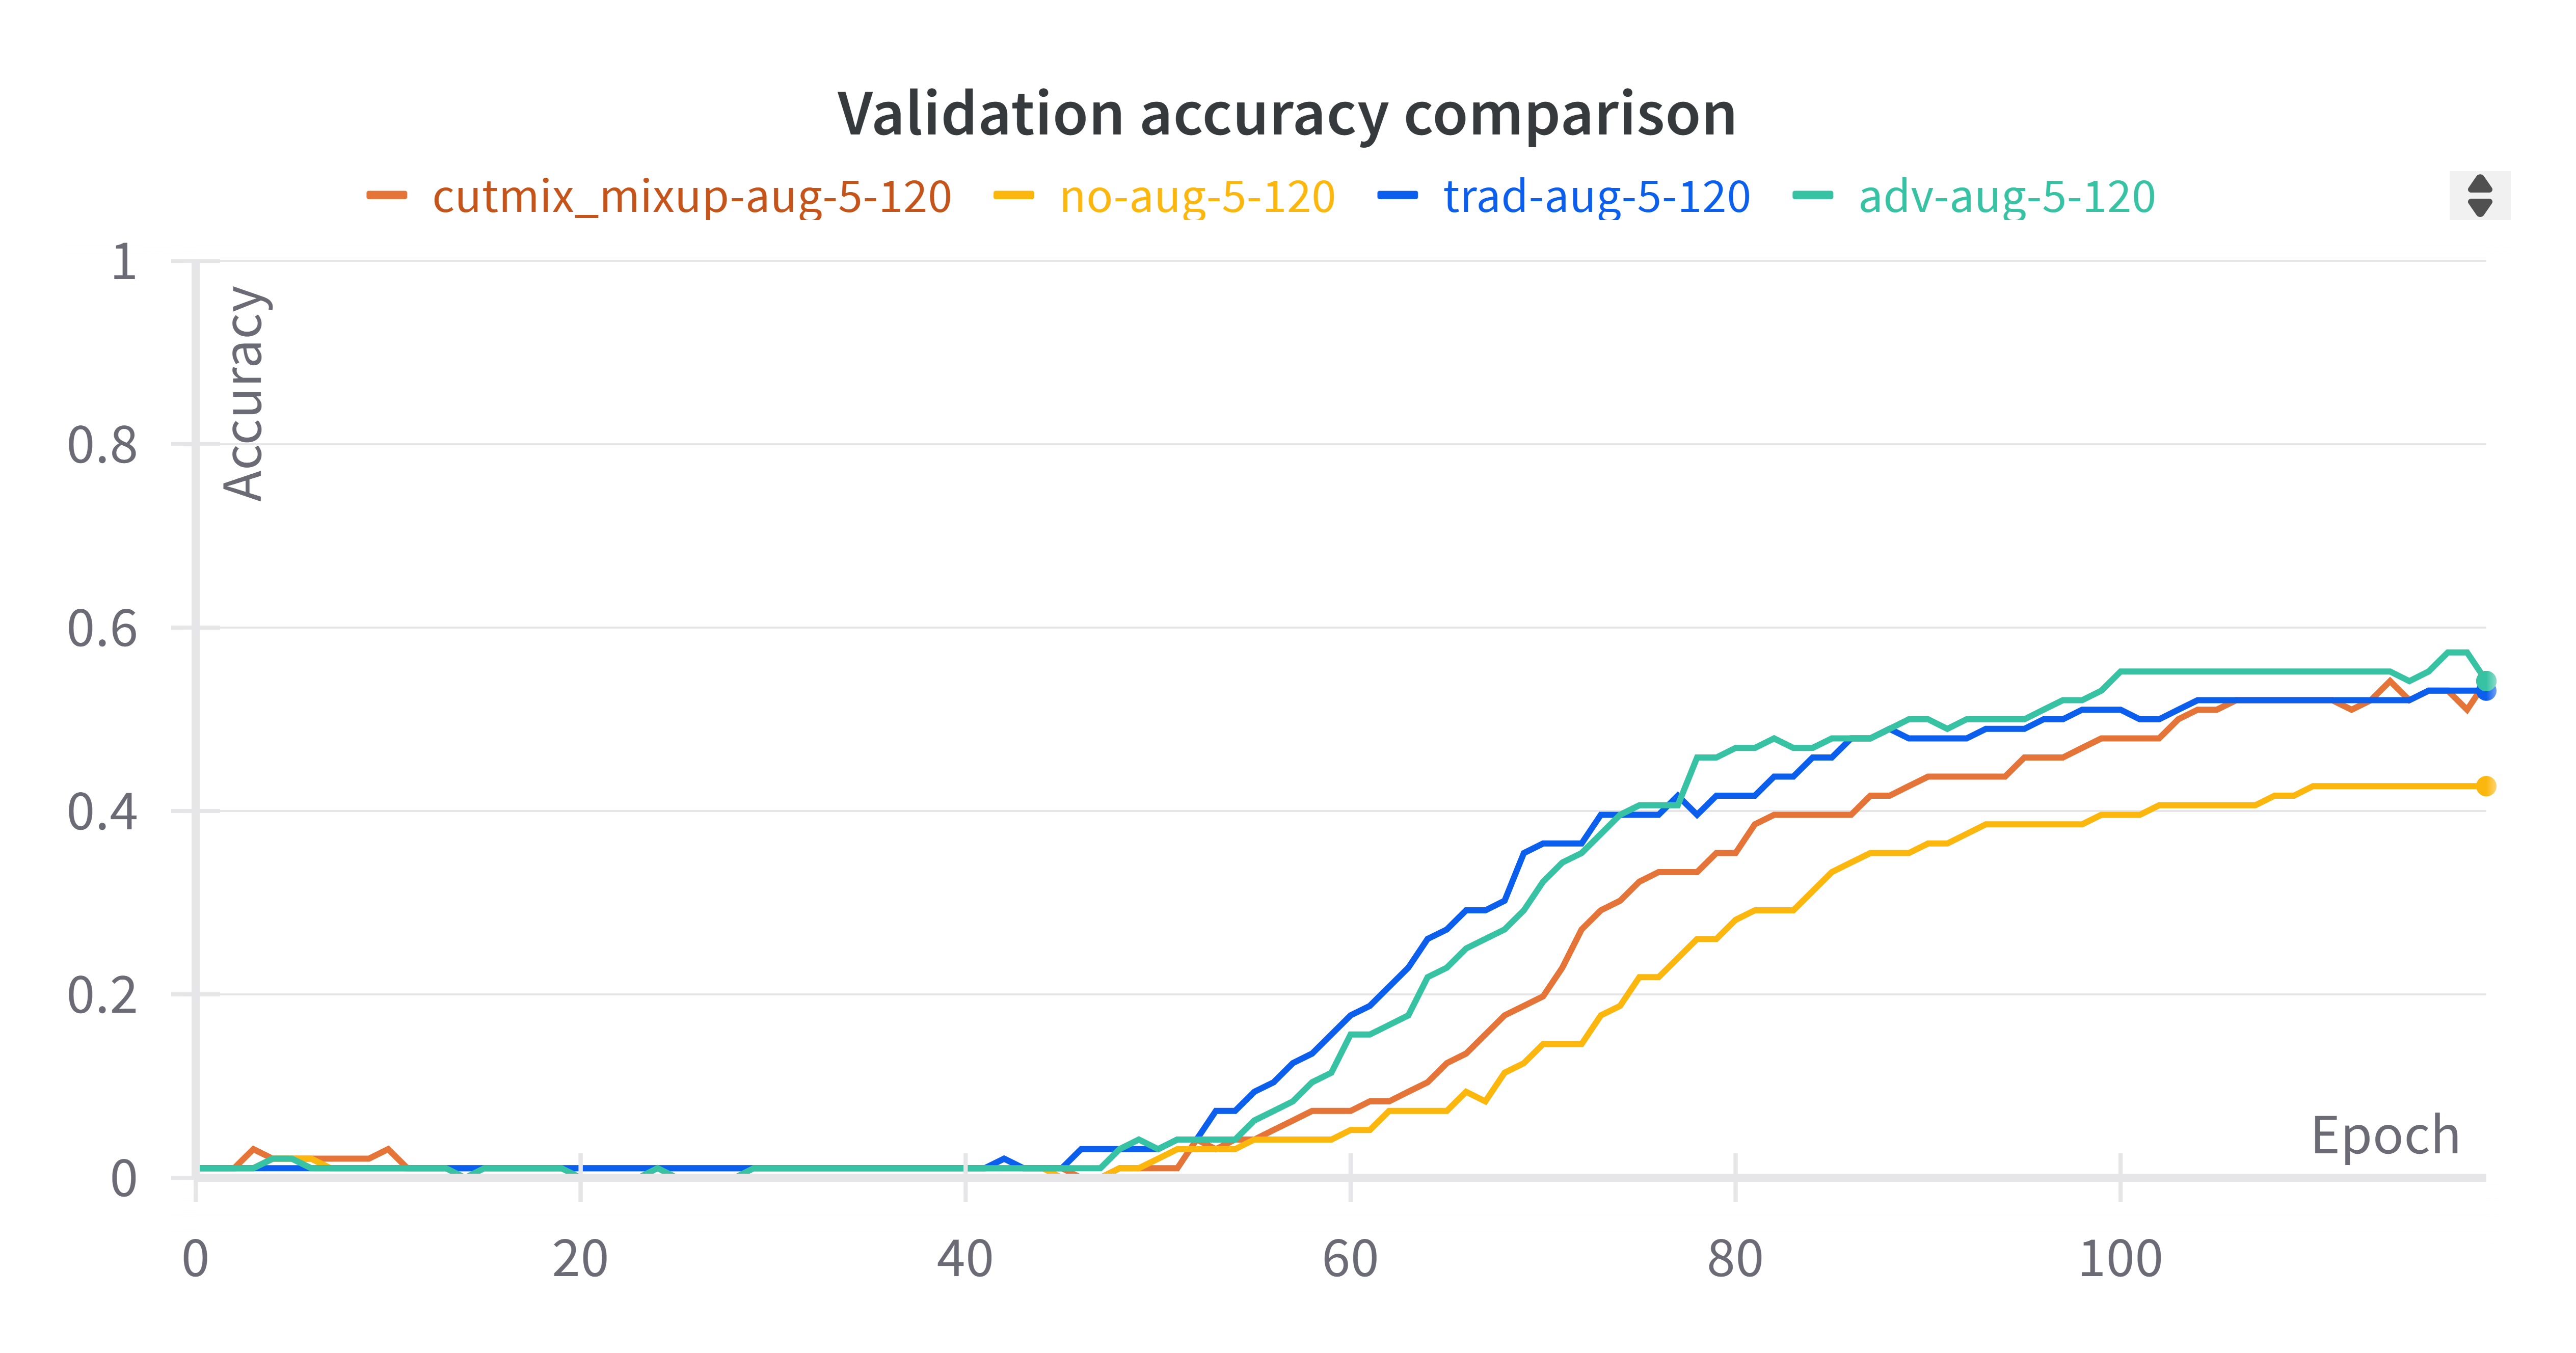
\includegraphics[width=\textwidth]{Images/oneshot/lc/val_acc_5.png}
        \caption{Validation accuracy - 5 samples}
    \end{subfigure}


    \begin{subfigure}[b]{0.77\textwidth}
        \centering
        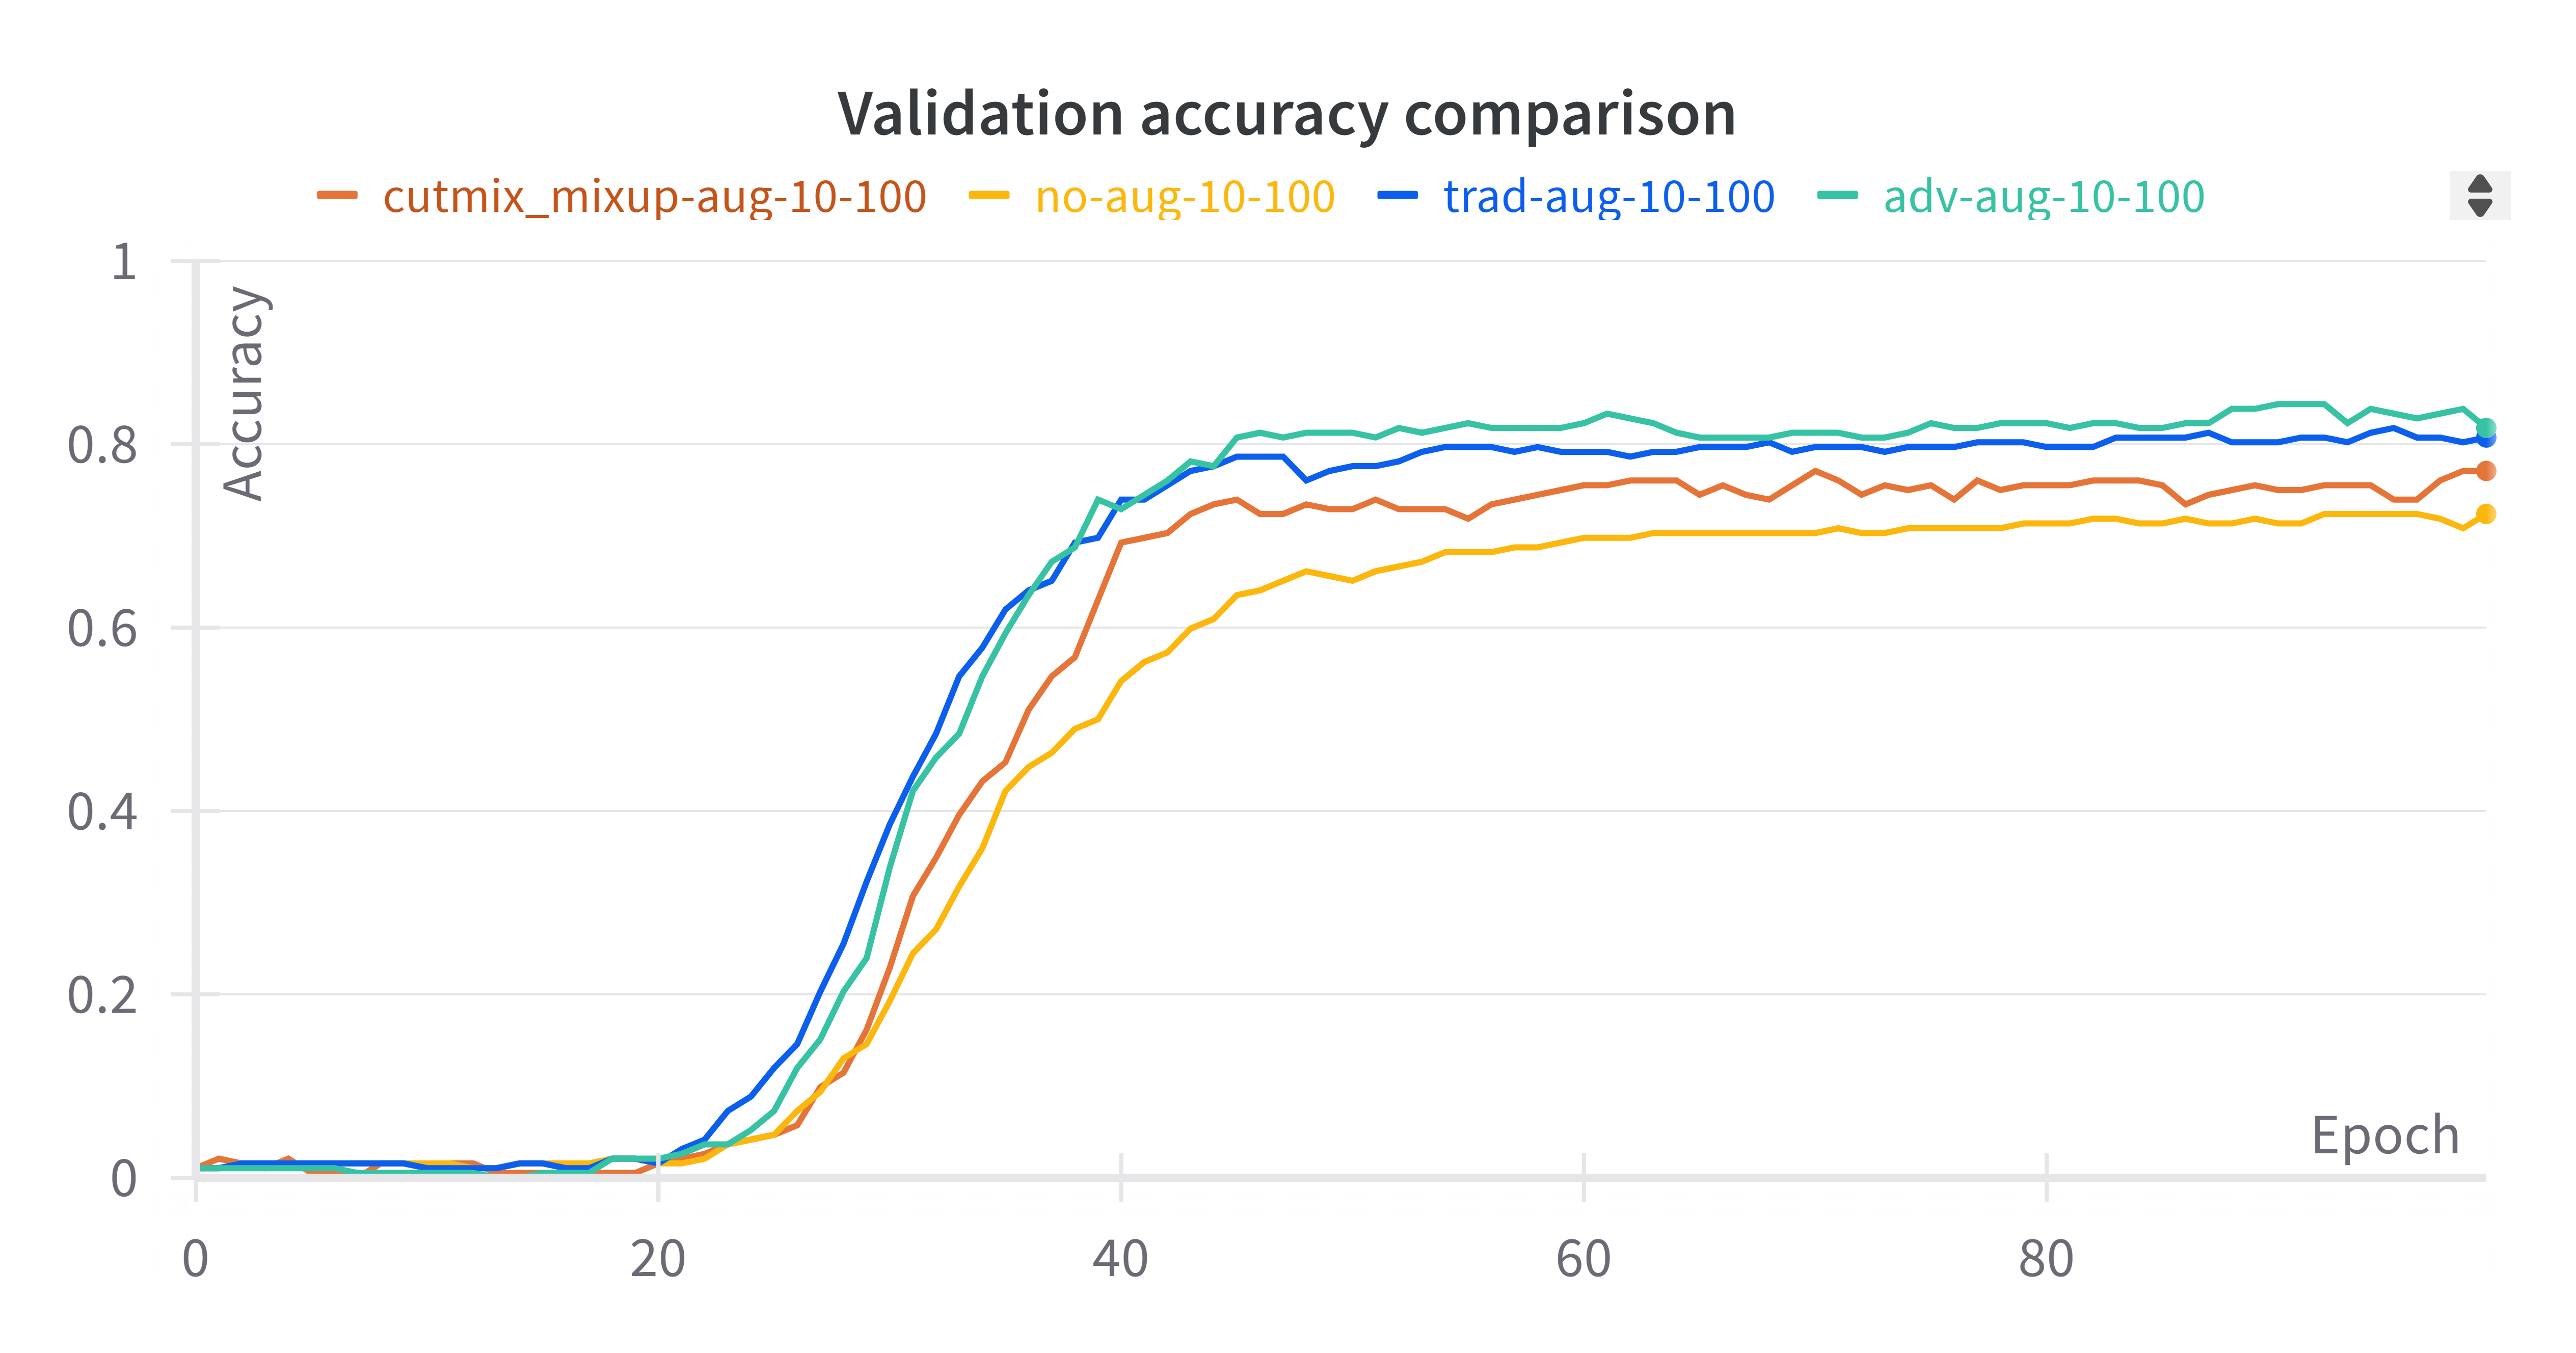
\includegraphics[width=\textwidth]{Images/oneshot/lc/val_acc_10.png}
        \caption{Validation accuracy - 10 samples}
    \end{subfigure}

    \begin{subfigure}[b]{0.77\textwidth}
        \centering
        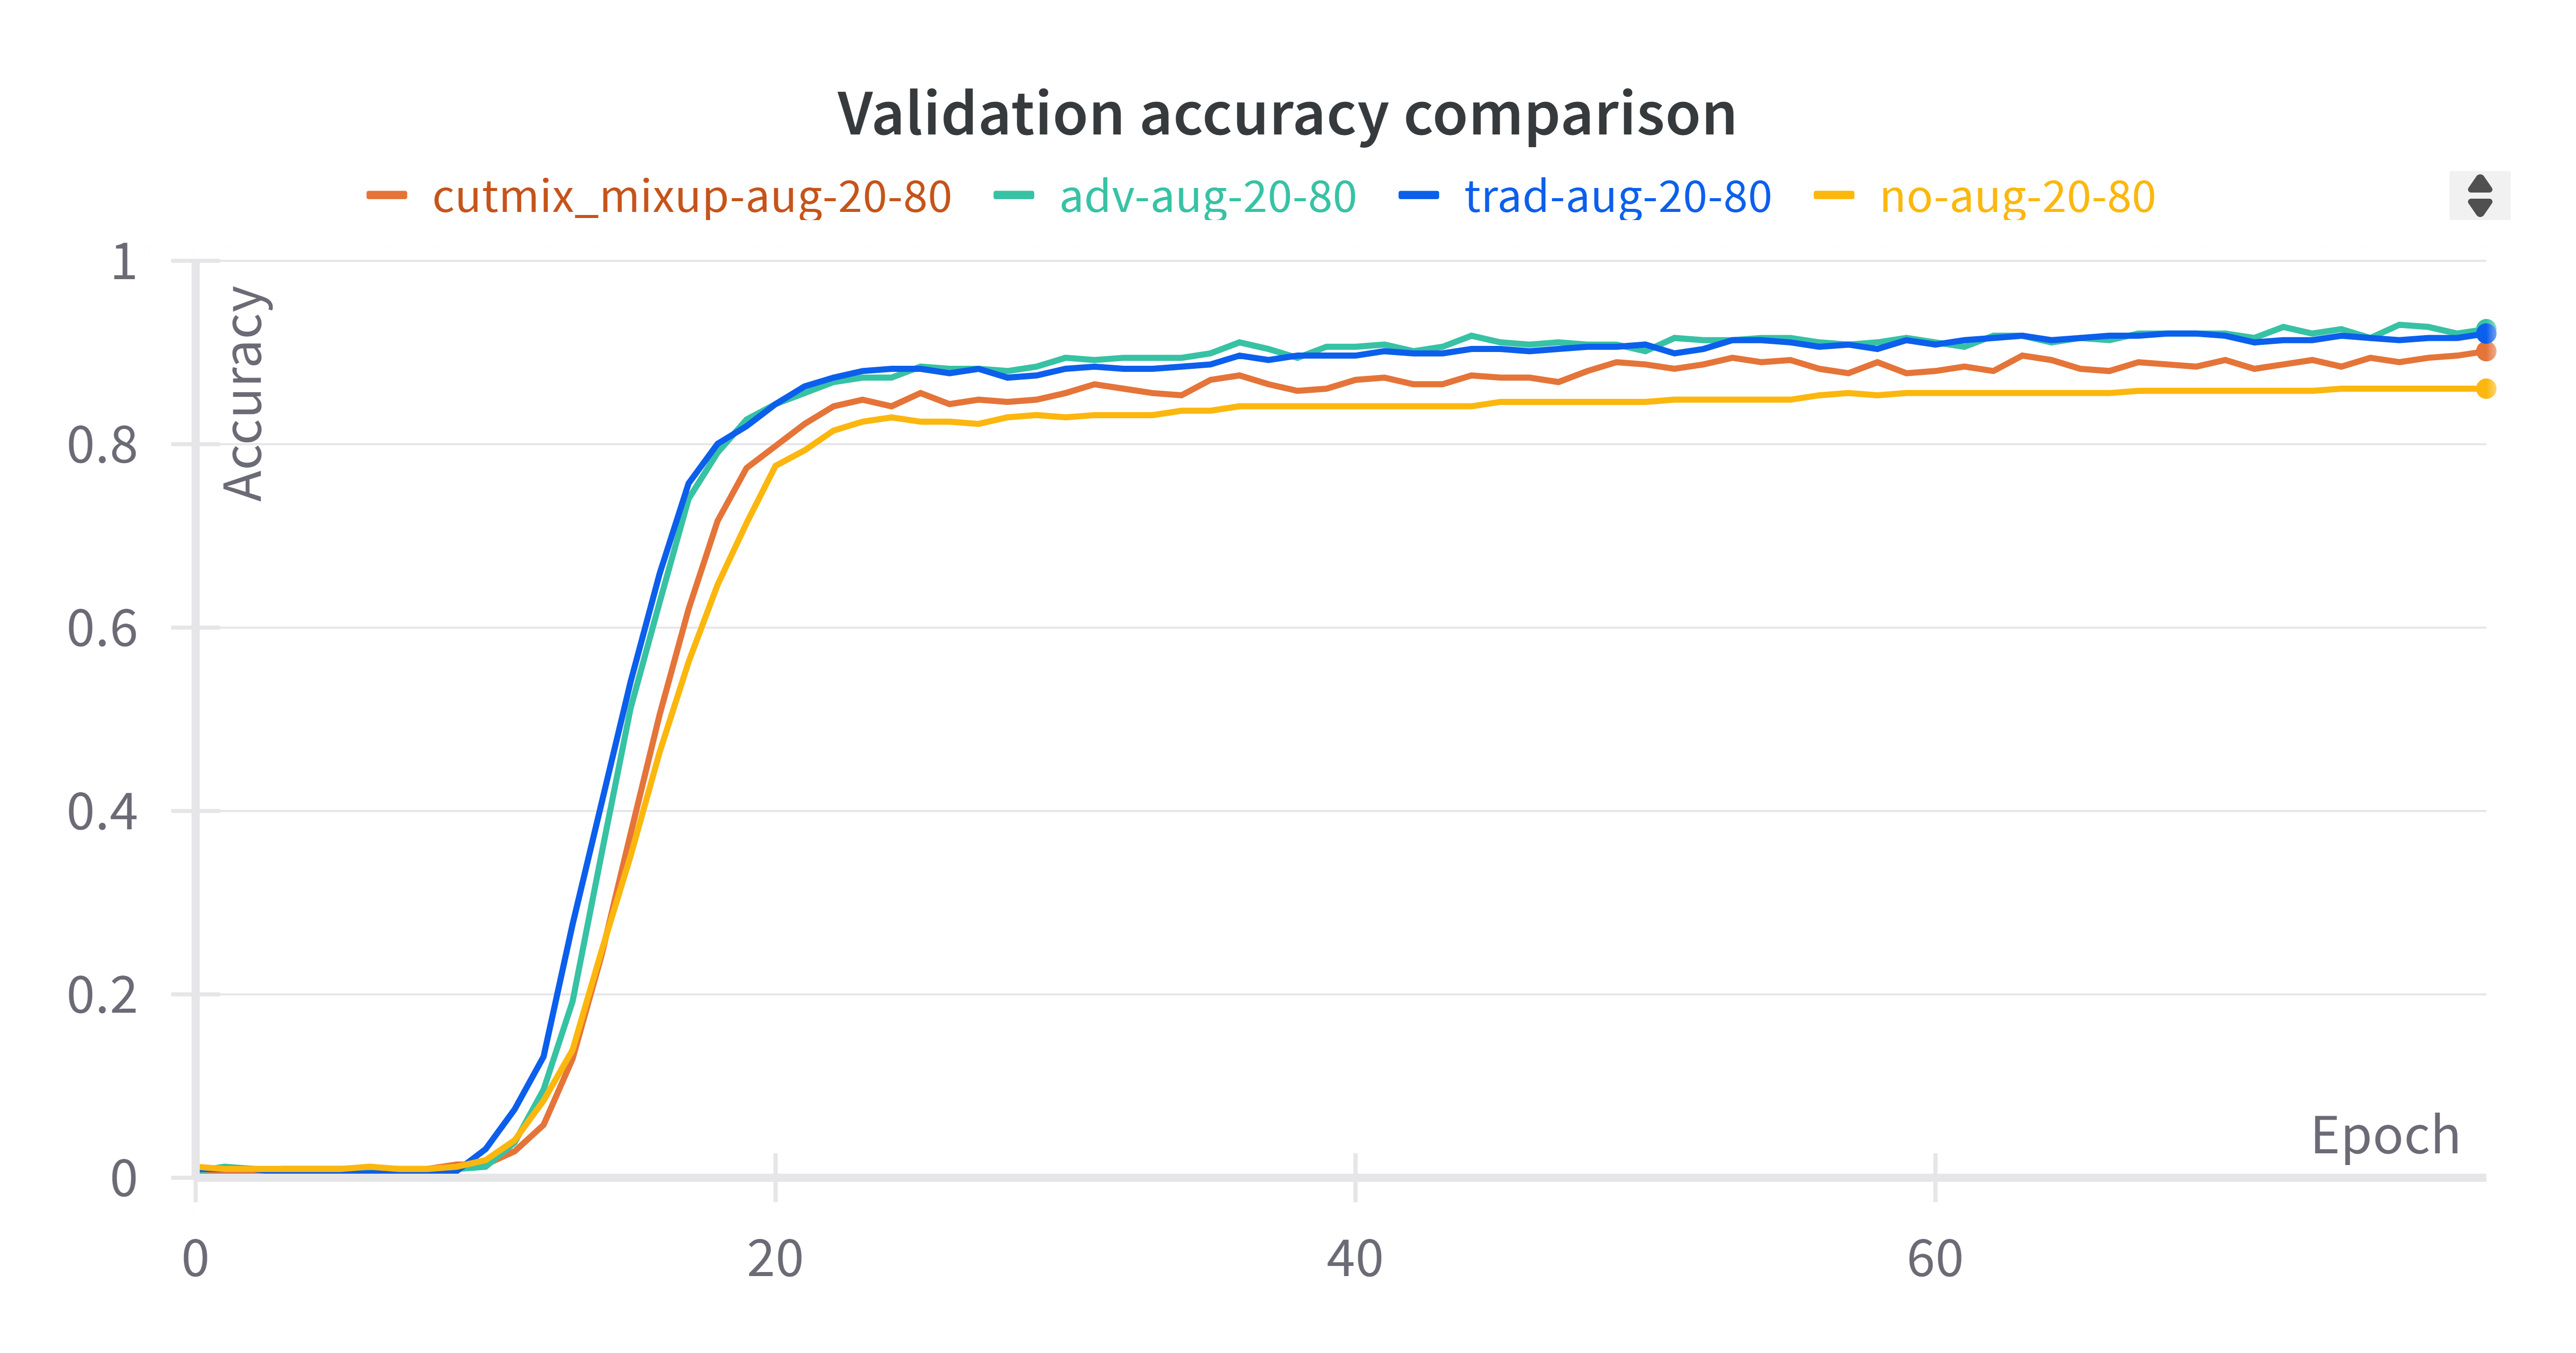
\includegraphics[width=\textwidth]{Images/oneshot/lc/val_acc_20.png}
        \caption{Validation accuracy - 20 samples}
    \end{subfigure}
    \caption{Validation learning curves for different sizes of Flowers 102 dataset.}
    \label{fig:oneshotLCsVal}
   
\end{figure}

For every dataset size, we observe that the training accuracy reaches 100\% when no augmentation or only traditional augmentation is used. However, with \textit{CutMix} and \textit{MixUp} data augmentation, training accuracy oscillates around 90\%. This is because \textit{MixUp} and \textit{CutMix} make the boundary between examples thinner, as the one-hot encoding is no longer a vector of only zeros and ones. Additionally, these techniques mix images among batches, and in \textit{CutMix}, important parts of the flower can be hidden, making the example difficult to classify correctly. All these factors together make the training process less stable, preventing 100\% accuracy from being reached.


More interesting conclusions can be obtained by looking at the validation accuracy learning curves. First of all, these experiments were repeated several times and the results were similar each time -- applying any kind of augmentation improves the performance of the network. Secondly, the smaller the dataset is, the more it benefits from applying augmentation.

For each dataset size, the influence of \textit{CutMix} and \textit{MixUp} augmentation is the lowest but for the smallest dataset improvement is quite impressive, and very close to other types of augmentations. Advanced augmentation, which combines all methods, yields the best results on the validation set but the difference between traditional augmentation and advanced augmentation is not very large. 

To enable better comparison between different datasets, Figure \ref{fig:oneshotLCSummary} was created. It displays all validation learning curves in a single plot. The colors are consistent: shades of yellow represent the dataset without augmentation, orange for \textit{CutMix} and \textit{MixUp}, blue for traditional augmentation, and green for advanced augmentation. Additionally, darker shades indicate larger dataset sizes. We can observe that larger datasets require fewer epochs to reach a saturation point in accuracy, where the model no longer shows improvement.

\begin{figure}[!h]
    \centering
    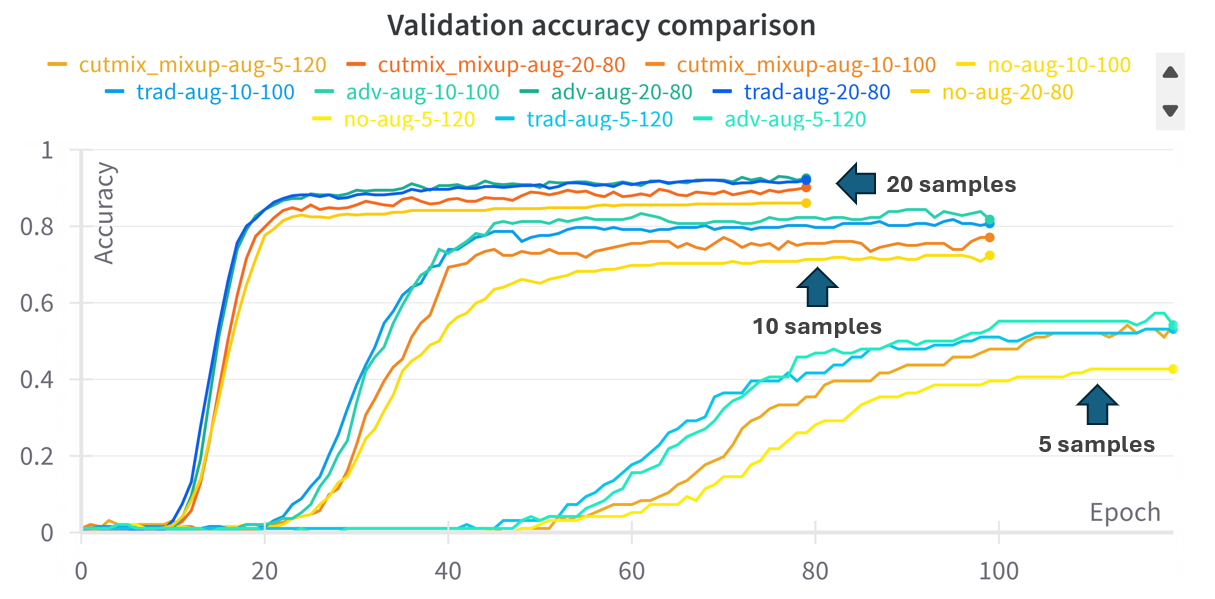
\includegraphics[width=\textwidth]{Images/oneshot/lc/summary_val_acc_improved2.png}
    \caption{Comparison of validation learning curves for all datasets and augmentation methods.}
    \label{fig:oneshotLCSummary}
\end{figure}

Moreover, no type of data augmentation can boost model performance as much as doubling the number of training examples. However, the model trained on a dataset with $10$ samples per class using advanced data augmentation performs almost as well as the model trained on a dataset with $20$ samples without any augmentation.

Table \ref{tab:augSampleComparison} presents results for the best epoch of each training as numerical values. Due to the small size of the validation set in limited data conditions, more general conclusions can be drawn by examining the test metrics.

\begin{table}[h!]
\centering
\caption{Augmentation comparison with different sample sizes.}
\begin{tabular}{| >{\centering\arraybackslash}m{1.5cm} | >{\centering\arraybackslash}m{2.2cm} !{\vrule width 1.5pt} >{\centering\arraybackslash}m{1.0cm} | >{\centering\arraybackslash}m{1.0cm} !{\vrule width 1.5pt} >{\centering\arraybackslash}m{1.0cm} | >{\centering\arraybackslash}m{1.0cm} !{\vrule width 1.5pt} >{\centering\arraybackslash}m{1.0cm} | >{\centering\arraybackslash}m{1.0cm} | >{\centering\arraybackslash}m{1.0cm} |}
\hline
\textbf{Samples} & \textbf{Augmentation} & \multicolumn{2}{c!{\vrule width 1.5pt}}{\textbf{Train}} & \multicolumn{2}{c!{\vrule width 1.5pt}}{\textbf{Val}} & \multicolumn{2}{c|}{\textbf{Test}} \\
\cline{3-8}
 &  & \textbf{Acc} & \textbf{AUC} & \textbf{Acc} & \textbf{AUC} & \textbf{Acc} & \textbf{F1} \\
\hline
\multirow{4}{*}{\makecell{5}} & \makecell{no-aug} & 99.22 & 1 & 42.71 & 0.376 & 42.74 & 40.59 \\
 & \makecell{traditional} & 98.96 & 1 & 53.13 & 0.579 & 64.47 & 63.43 \\
 & \makecell{cutmix-mixup} & 94.27 & 0.766 & 54.17 & 0.521 & 56.9 & 54.61 \\
 & \makecell{advanced} & 94.79 & 0.592 & 57.29 & 0.627 & 65.93 & 64.56 \\
\hline
\multirow{4}{*}{\makecell{10}} & \makecell{no-aug} & 99 & 1 & 72.4 & 0.743 & 66.79 & 65.75 \\
 & \makecell{traditional} & 98.87 & 1 & 81.77 & 0.885 & 80.65 & 80.2 \\
 & \makecell{cutmix-mixup} & 94 & 0.6544 & 77.08 & 0.851 & 73.93 & 72.93 \\
 & \makecell{advanced} & 87.25 & 0.615 & 84.38 & 0.910 & 80.34 & 79.73 \\
\hline
\multirow{4}{*}{\makecell{20}} & \makecell{no-aug} & 98.94 & 1 & 86.06 & 91.54 & 81.62 & 81.17 \\
 & \makecell{traditional} & 98.94 & 1 & 92.07 & 0.966 & 88.83 & 88.57 \\
 & \makecell{cutmix-mixup} & 92.19 & 0.648 & 90.14 & 95.04 & 86.87 & 86.34 \\
 & \makecell{advanced} & 91.62 & 0.579 & 93.03 & 0.968 & 88.22 & 87.82 \\
\hline
\end{tabular}
\label{tab:augSampleComparison}
\end{table}

Examining the results of the models trained on the dataset with $5$ samples for each species of flower, we see that the greatest improvement comes from using advanced augmentation techniques. Test accuracy increases from 42.74\% to 65.93\% — a significant improvement of over 23 percentage points for accuracy and 24 percentage points for F1 score. Traditional augmentation gives almost the same improvement, only 1 percentage point less for both metrics. 

For a dataset with $10$ samples per class, the improvement is also notable. All the metrics show enhancement, and while advanced augmentation shows slightly better validation metrics compared to traditional augmentation, the test metrics reveal that traditional augmentation performs slightly better than advanced augmentation.

Even though the validation metrics with augmentation applied on the dataset with $20$ samples per class were almost as good as the ones obtained for the full dataset presented in the previous section, test metrics turned out to be slightly worse. Nonetheless, with this dataset size, data augmentation techniques enable achieving almost 90\% accuracy on the test set with $102$ classes.

Test metrics presented in Table \ref{tab:augSampleComparison} also confirm that data augmentation applied to the dataset can make the model perform almost as well as the one trained on two times bigger dataset. When we apply advanced augmentation to the dataset with $5$ samples per category, we obtain $65.93\%$ test accuracy which is only $0.86$ percentage points less than the one trained on the dataset with 10 samples per category. Similarly, on the dataset with $10$ samples we can achieve $80.65\%$ accuracy, which is $0.97$ percentage points less than for a two times larger dataset.

Figure \ref{fig:testMetricsOneshot} presents test set metrics in the form of bar plots and enable visual comparison of results. The name of each bar indicates the augmentation type and number of samples in each class.

\begin{figure}[!h]
    \centering
    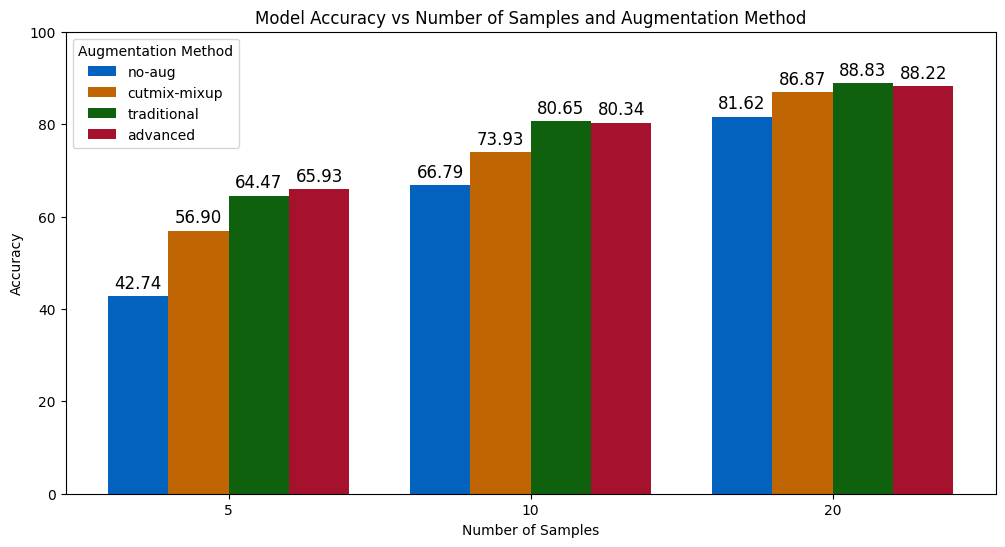
\includegraphics[width=0.95\textwidth]{Images/oneshot/oneshot_test_bar_plot.png}
    \caption{Comparison of test metric values for different augmentation methods and class sizes.}
    \label{fig:testMetricsOneshot}
\end{figure}

Confusion matrices for the top $10$ worst-performing classes in the dataset with $5$ samples per category were plotted in Figure \ref{fig:confMatricesOneshot}. On the left side, we can see that none of these classes are correctly classified. However, when advanced data augmentation methods are applied, the model learns features that enable it to correctly classify some examples, improving overall performance. Similar to the confusion matrix for the full dataset, the confusion matrix still shows no improvement for \textit{blackberry lily}, despite the dataset being balanced. It means that data augmentation applied to the dataset does not work for all classes and some directed approach should be used to improve the performance of these categories.

\begin{figure}[!htb]
    \centering
    \begin{subfigure}[b]{0.49\textwidth}
        \centering
        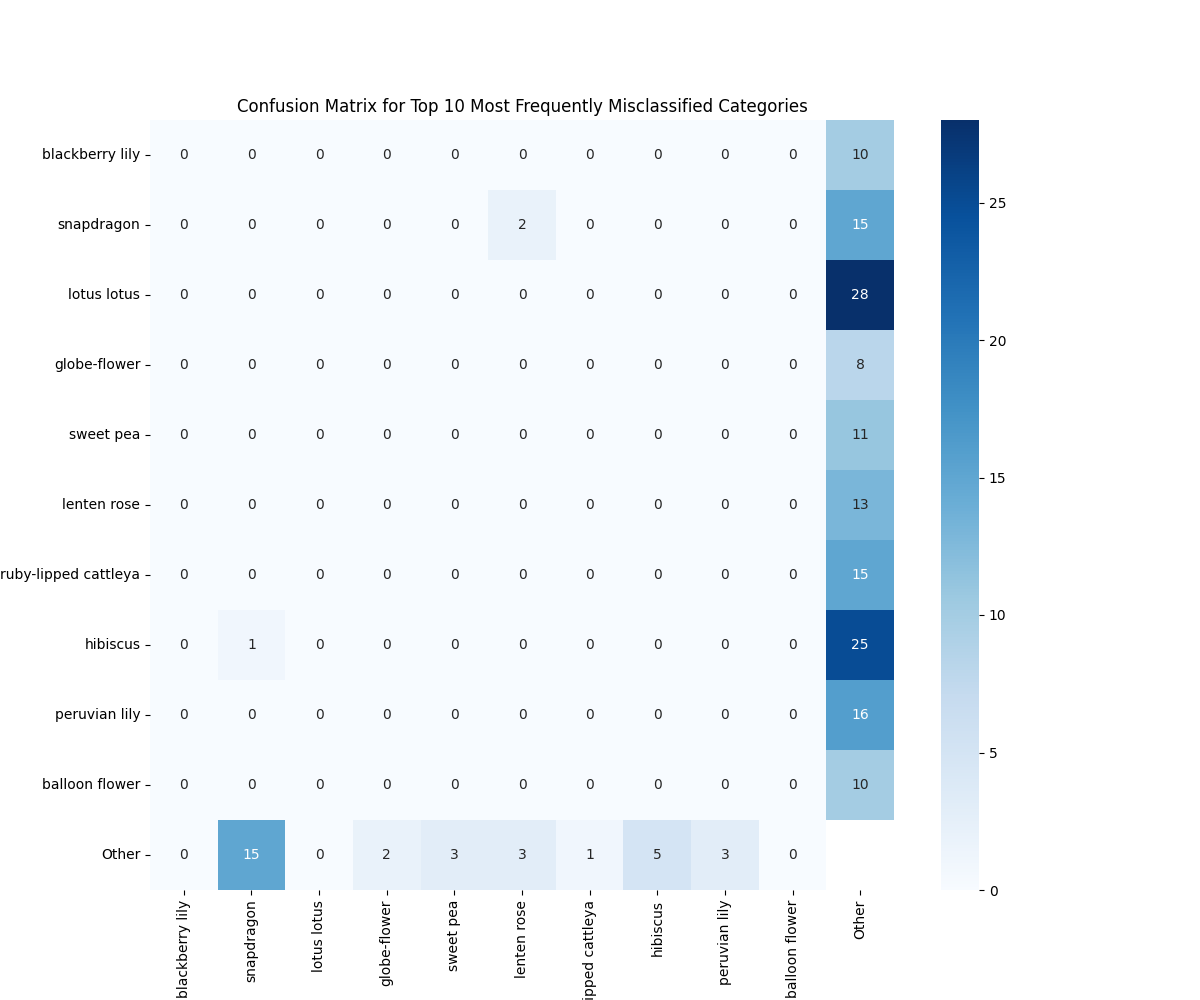
\includegraphics[width=\textwidth]{Images/oneshot/cm/no_aug_cm.png}
        \subcaption{Without augmentation}
    \end{subfigure}
    % \hfill
    \begin{subfigure}[b]{0.49\textwidth}
        \centering
        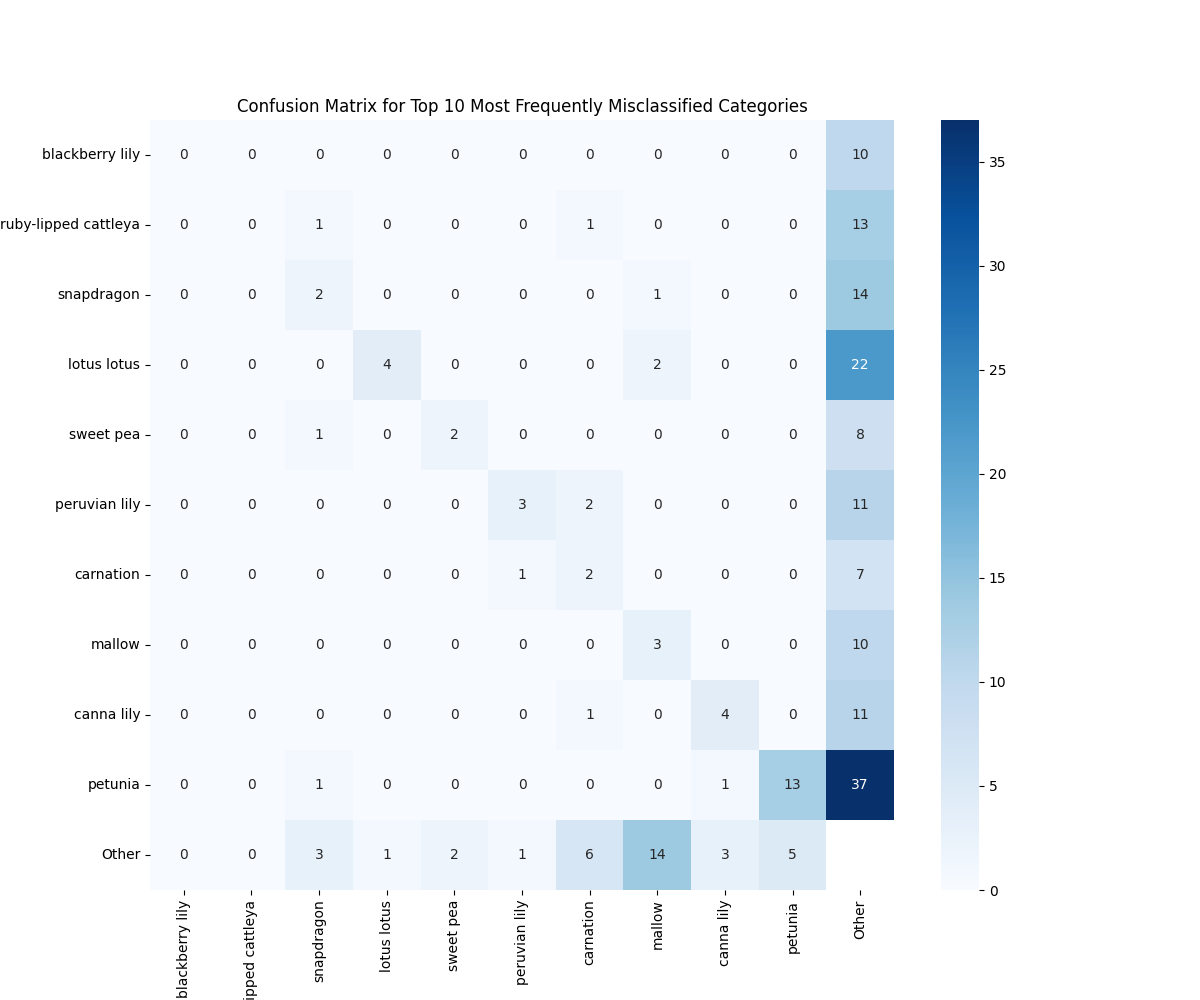
\includegraphics[width=\textwidth]{Images/oneshot/cm/adv_aug_cm.png}
        \subcaption{With advanced augmentation}
    \end{subfigure}
    \caption{Confusion matrices for the top 10 worst-performing species of flowers on Oneshot dataset.}
    \label{fig:confMatricesOneshot}
\end{figure}

Looking at saliency maps for models trained on the dataset containing $10$ samples of each class, unlike for the models trained on the full dataset, we can see a big difference not only for examples misclassified for the worse performing network but also for examples correctly classified by both models. Figure \ref{fig:saliencySummary1} illustrates several such cases. The better-performing models show more centralized focus and attention on the more distinctive parts of the flowers.


\begin{figure}[!h]
    \centering
    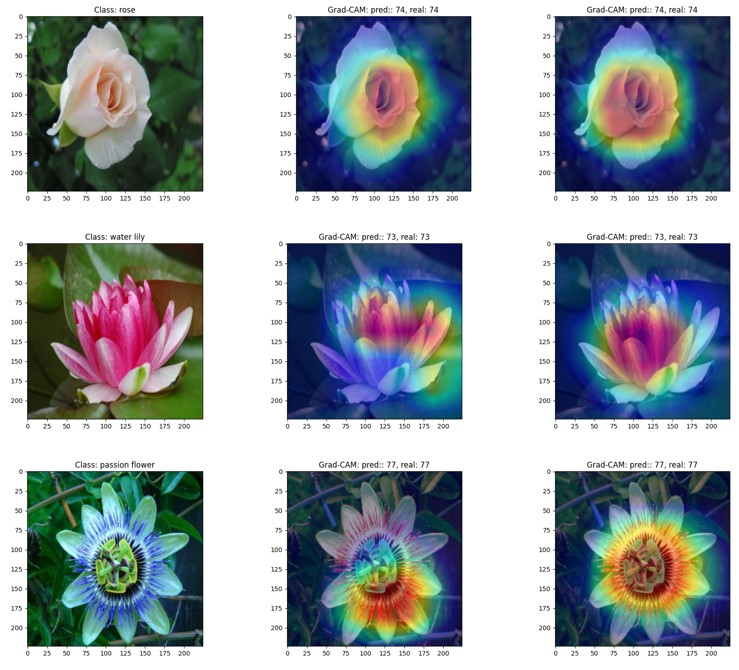
\includegraphics[width=0.55\textwidth]{Images/saliency-oneshot/both_ok_summary.jpg}
    \caption{Saliency maps for cases where both models made the \textbf{same} predictions.}
    \label{fig:saliencySummary1}
\end{figure}

The difference is even more crucial for examples wrongly classified by the first model. Figure \ref{fig:saliencySummary2} visualizes this.

\begin{figure}[!h]
    \centering
    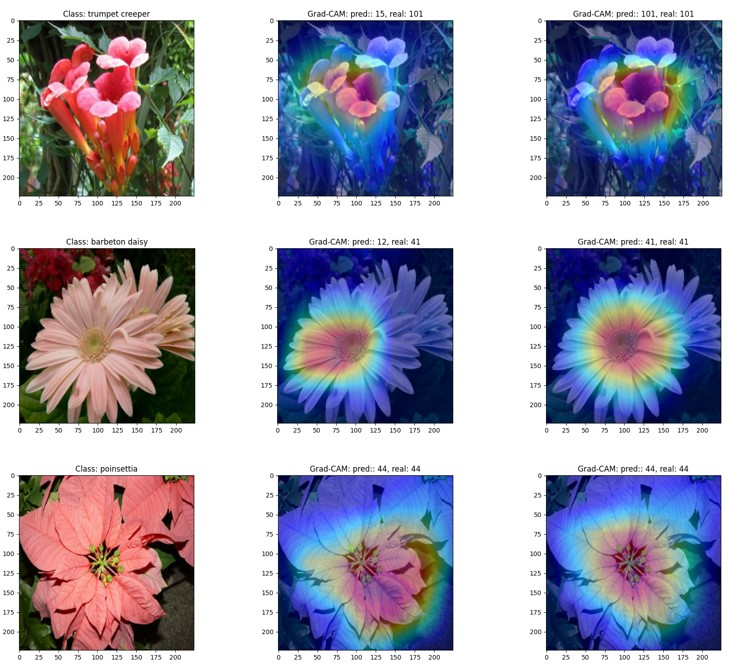
\includegraphics[width=0.55\textwidth]{Images/saliency-oneshot/diff_summary.jpg}
    \caption{Saliency maps for cases where both models made the \textbf{different} predictions.}
    \label{fig:saliencySummary2}
\end{figure}

\subsection{GTZAN}
\label{ssec:resultsGTZAN}

The next set of experiments was conducted on the GTZAN dataset. The main objective was to explore new augmentation methods and their impact on the convolutional networks' performance. For this dataset, all augmentation techniques were applied together, as previous experiments demonstrated that combining augmentation methods improves results. Each augmentation technique had an independent probability of 50\%. 

The biggest challenge in performing these experiments was that some augmentations had to be applied at the audio wave level. This made using the pre-calculated spectrograms in the data set was impossible. Instead, the process involved loading an audio signal, applying audio augmentation techniques, transforming it into spectrograms, and then applying augmentations at the spectrogram level. This process was time-consuming and massively slowed down the training. Although it was theoretically possible to create and save an augmented dataset before training, this would reduce the randomness of data augmentation and potentially lower its effectiveness.

\begin{figure}[!htb]
    \centering
    \begin{subfigure}{0.8\textwidth}
        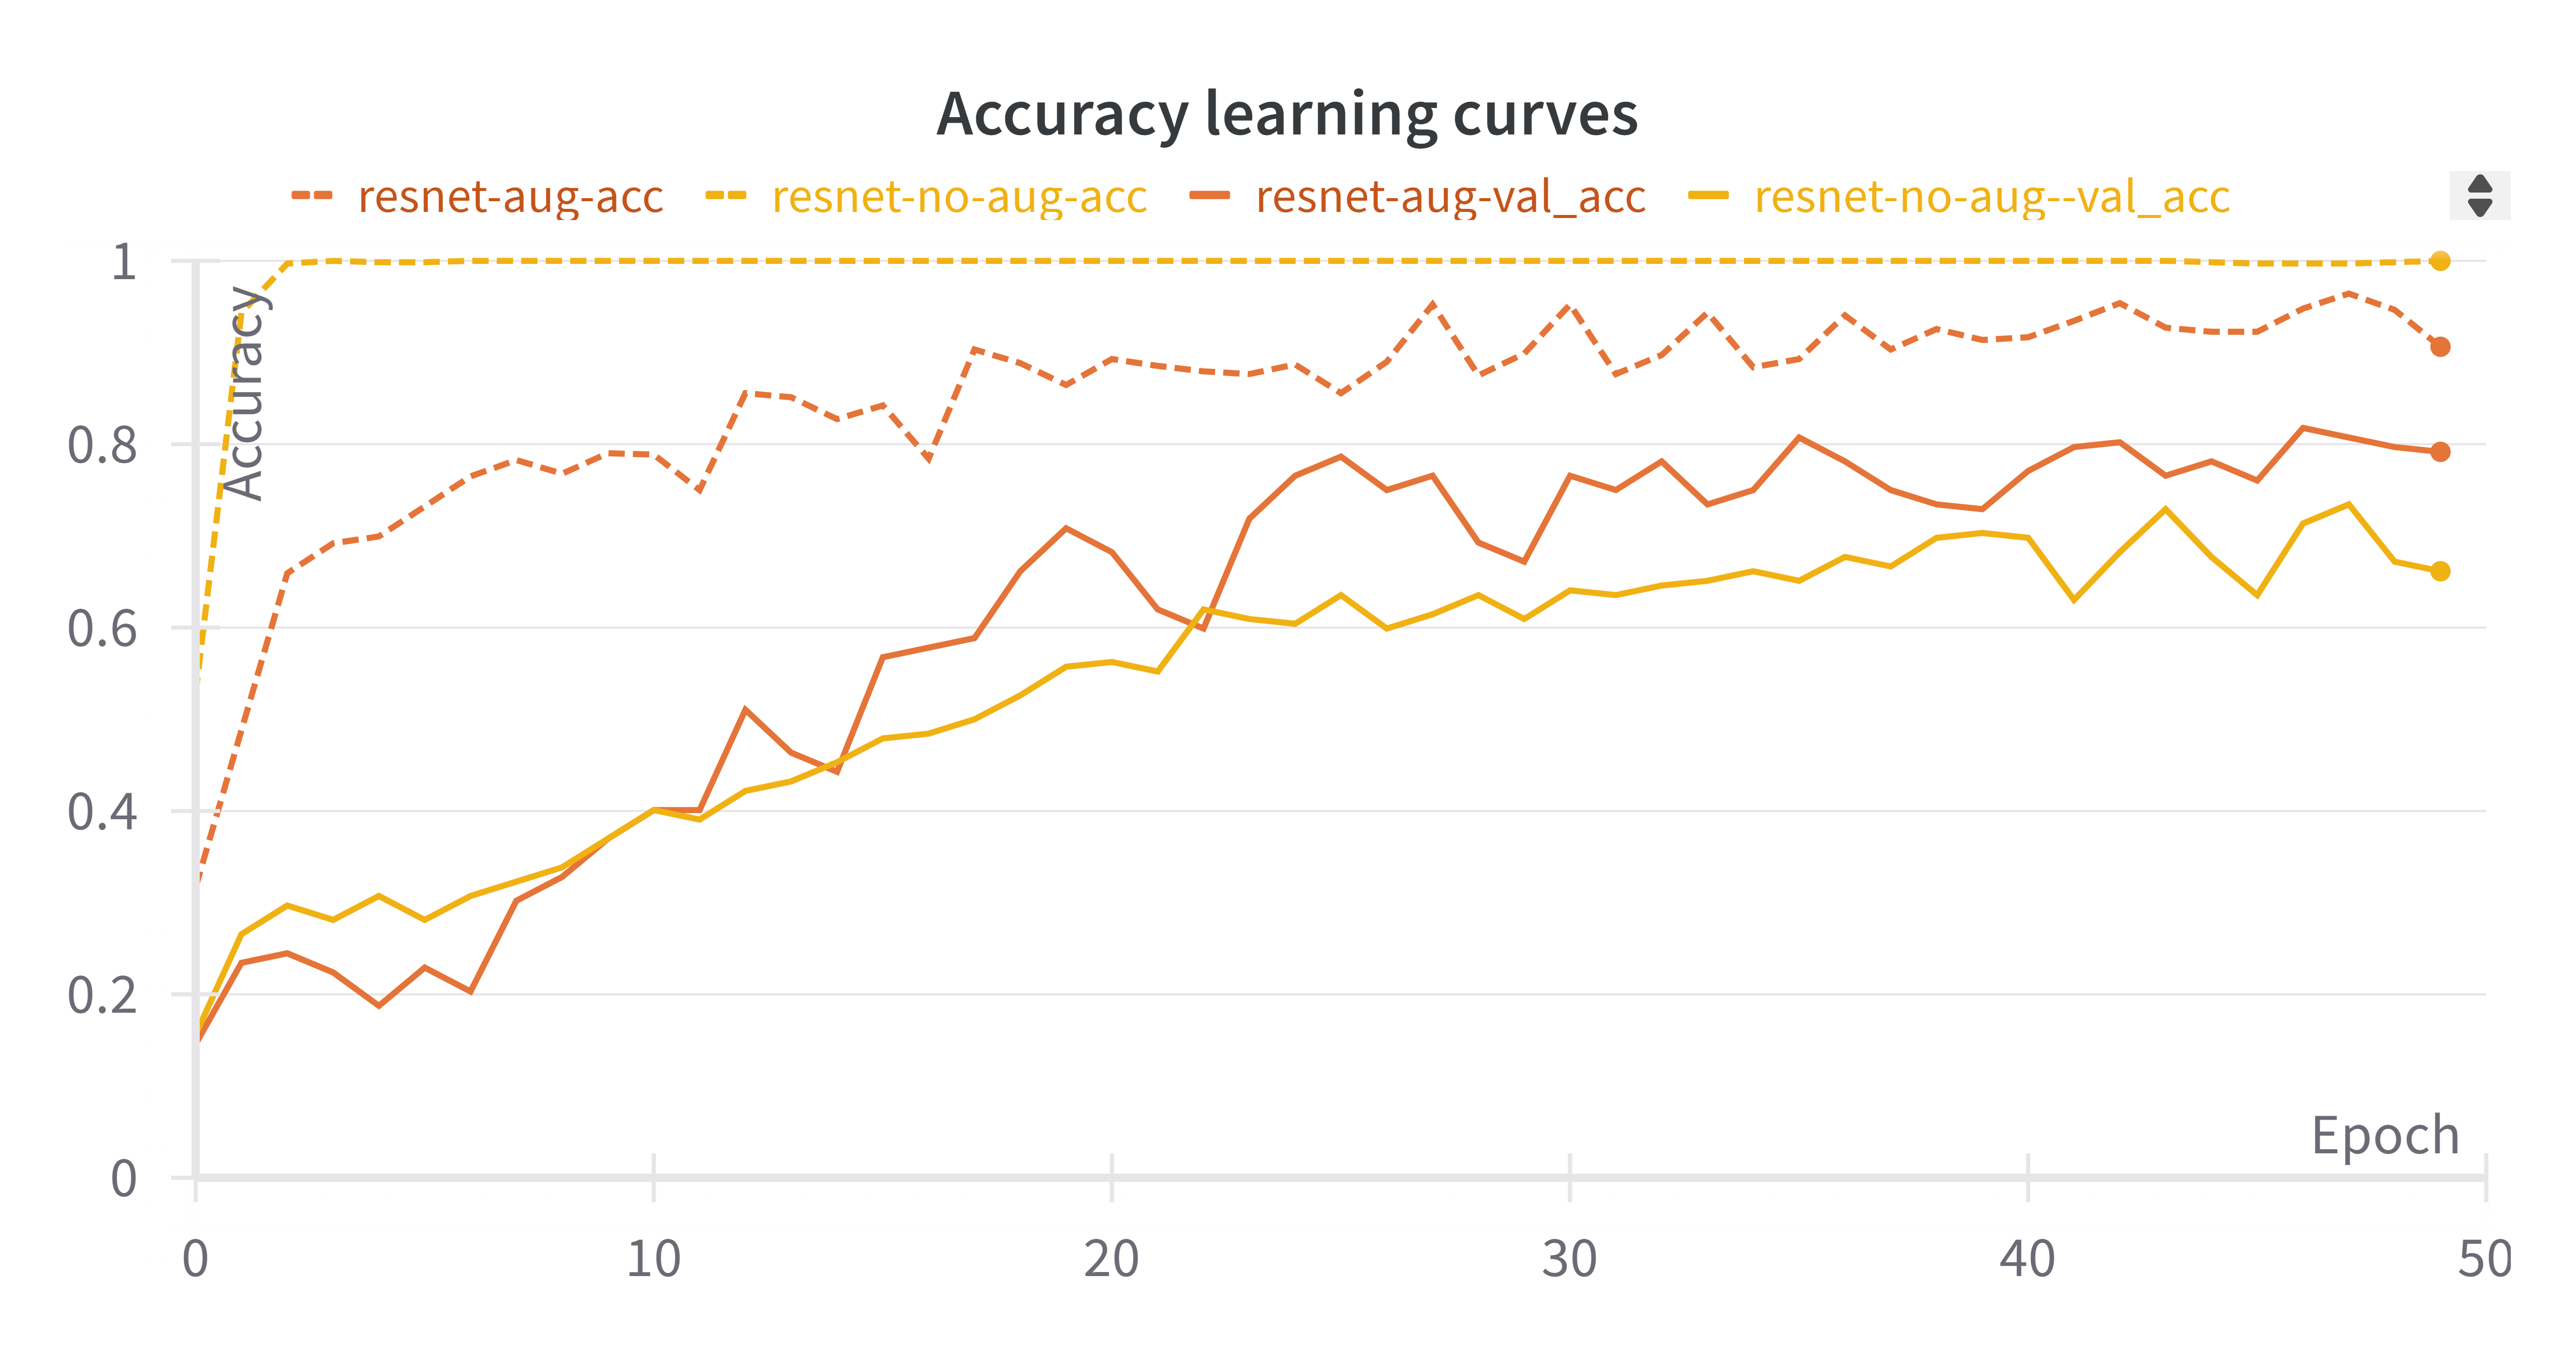
\includegraphics[width=\textwidth]{Images/gtzan_plots/lc/resnet_acc_lc.png}
        \caption{Accuracy}
    \end{subfigure}
    \vspace{0.3cm}
    % \hfill
    \begin{subfigure}{0.8\textwidth}
        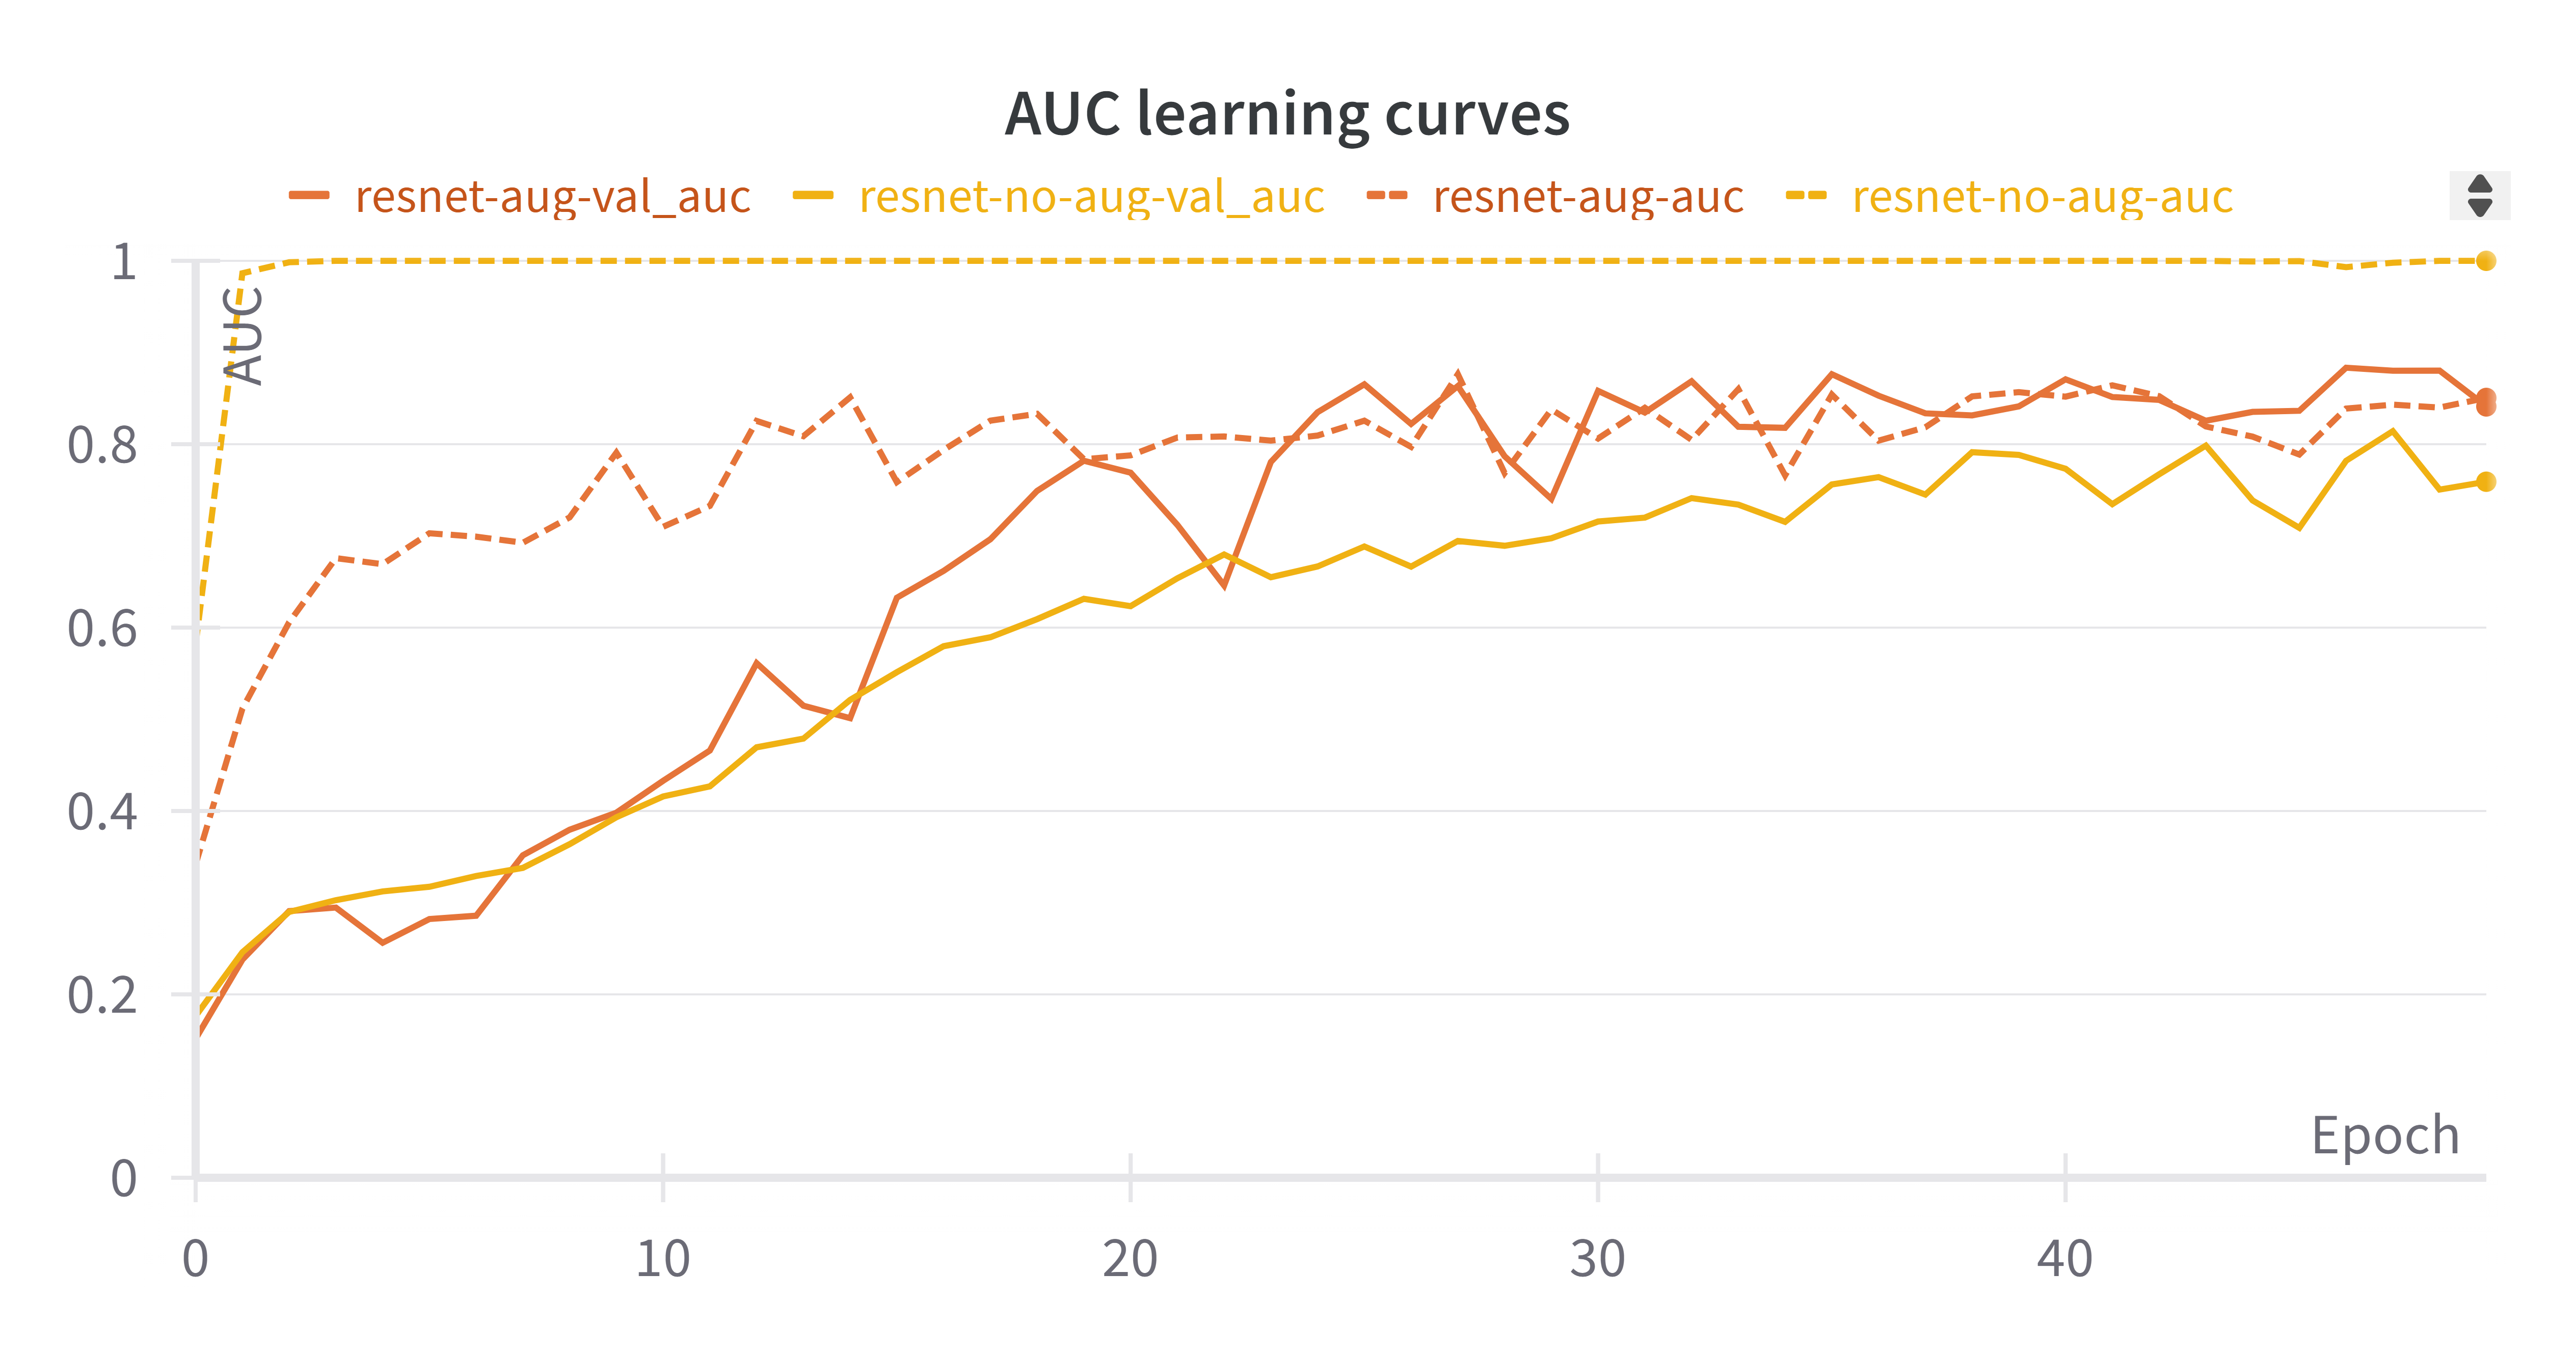
\includegraphics[width=\textwidth]{Images/gtzan_plots/lc/resnet_auc_lc.png}\
        \caption{AUC}
    \end{subfigure}
    \vspace{0.3cm}
    \caption{Training and validation learning curves comparison for different augmentation types.}
    \label{fig:GTZANLearningCurves}
\end{figure}

First, the model based on \textit{ResNet} architecture was trained. Figure \ref{fig:GTZANLearningCurves} shows a comparison of learning curves of models trained on the datasets with and without data augmentation applied.

Looking at the learning curves, we can observe that the model's performance improved due to the augmentation.
Without the data augmentation model overfits the training data reaching 100\% accuracy in just 3 epochs and keeping this value until the end of training. In contrast, using data augmentation, we make it impossible for the model to memorize the data and the network learns through all epochs, never reaching 100\% training accuracy.

Focusing on validation accuracy, it becomes clear that without the use of a data augmentation model heavily overfits. The difference between training and validation accuracy is more than 20 percentage points, with training accuracy at 100\%. In contrast, data augmentation improves the validation accuracy by over 8 percentage points and decreases the gap between training and validation accuracy.

Table \ref{tab:gtzanMetrics} presents the numerical results of the experiments described above. The model from the best epoch was selected based on the highest validation accuracy. Notably, with data augmentation applied, the AUC on the validation set is higher than that on the training set, indicating better generalization.

\begin{table}[h!]
\centering
\caption{ResNet metrics comparison.}
\begin{tabular}{| >{\centering\arraybackslash}m{2.5cm} !{\vrule width 1.5pt} >{\centering\arraybackslash}m{1.0cm} | >{\centering\arraybackslash}m{1.0cm} !{\vrule width 1.5pt} >{\centering\arraybackslash}m{1.0cm} | >{\centering\arraybackslash}m{1.0cm} !{\vrule width 1.5pt} >{\centering\arraybackslash}m{1.0cm}|}
\hline
\multirow{2}{*}{\textbf{Augmentation}} & \multicolumn{2}{c!{\vrule width 1.5pt}}{\textbf{Train}} & \multicolumn{2}{c!{\vrule width 1.5pt}}{\textbf{Val}} \\
\cline{2-5}
 & \textbf{Acc} & \textbf{AUC} & \textbf{Acc} & \textbf{AUC} \\
\hline
no-aug & 99.70 & 99.79 & 73.44 & 81.43 \\
\hline
advanced & 94.79 & 83.89 & 81.77 & 88.34 \\
\hline
\end{tabular}
\label{tab:gtzanMetrics}
\end{table}

Figure \ref{fig:gtzanTestBars} presents metrics calculated on the test set as bar plots. The test set accuracy is higher than that of the validation set. Both models exhibit higher precision than recall which is equal to accuracy because of the utilization of micro-averaging. Additionally, all metrics improved significantly due to the application of data augmentation. 

\begin{figure}[!h]
    \centering
    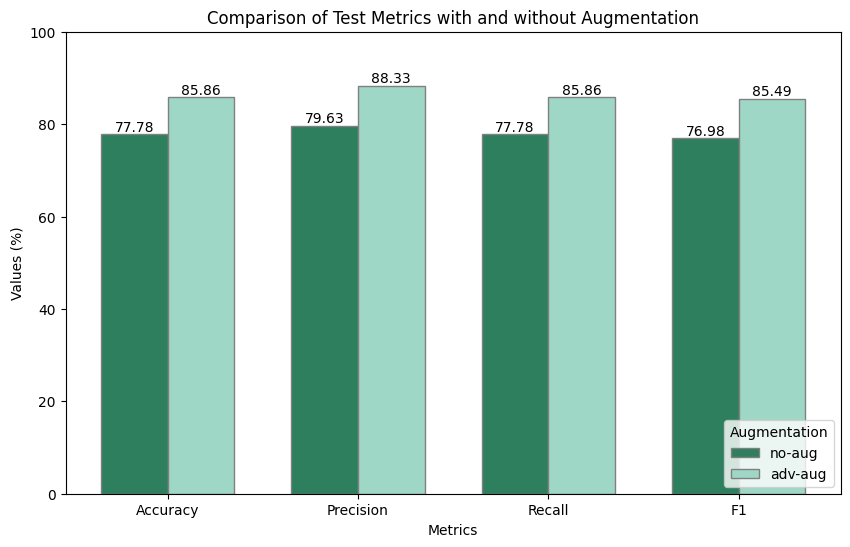
\includegraphics[width=0.9\textwidth]{Images/gtzan_plots/test_metrics_gtzan.png}
    \caption{Comparison of metrics calculated on the test set for the models trained with and without augmentation.}
    \label{fig:gtzanTestBars}
\end{figure}


Next, as for the Flowers 102 dataset, \textit{EfficientNet} was used as a base model to test the influence of data augmentation on another architecture. Learning curves for this network are visible in Figure \ref{fig:gtzanEfficientLC}.

\begin{figure}[!htb]
    \centering
    \begin{subfigure}{\textwidth}
        \centering
        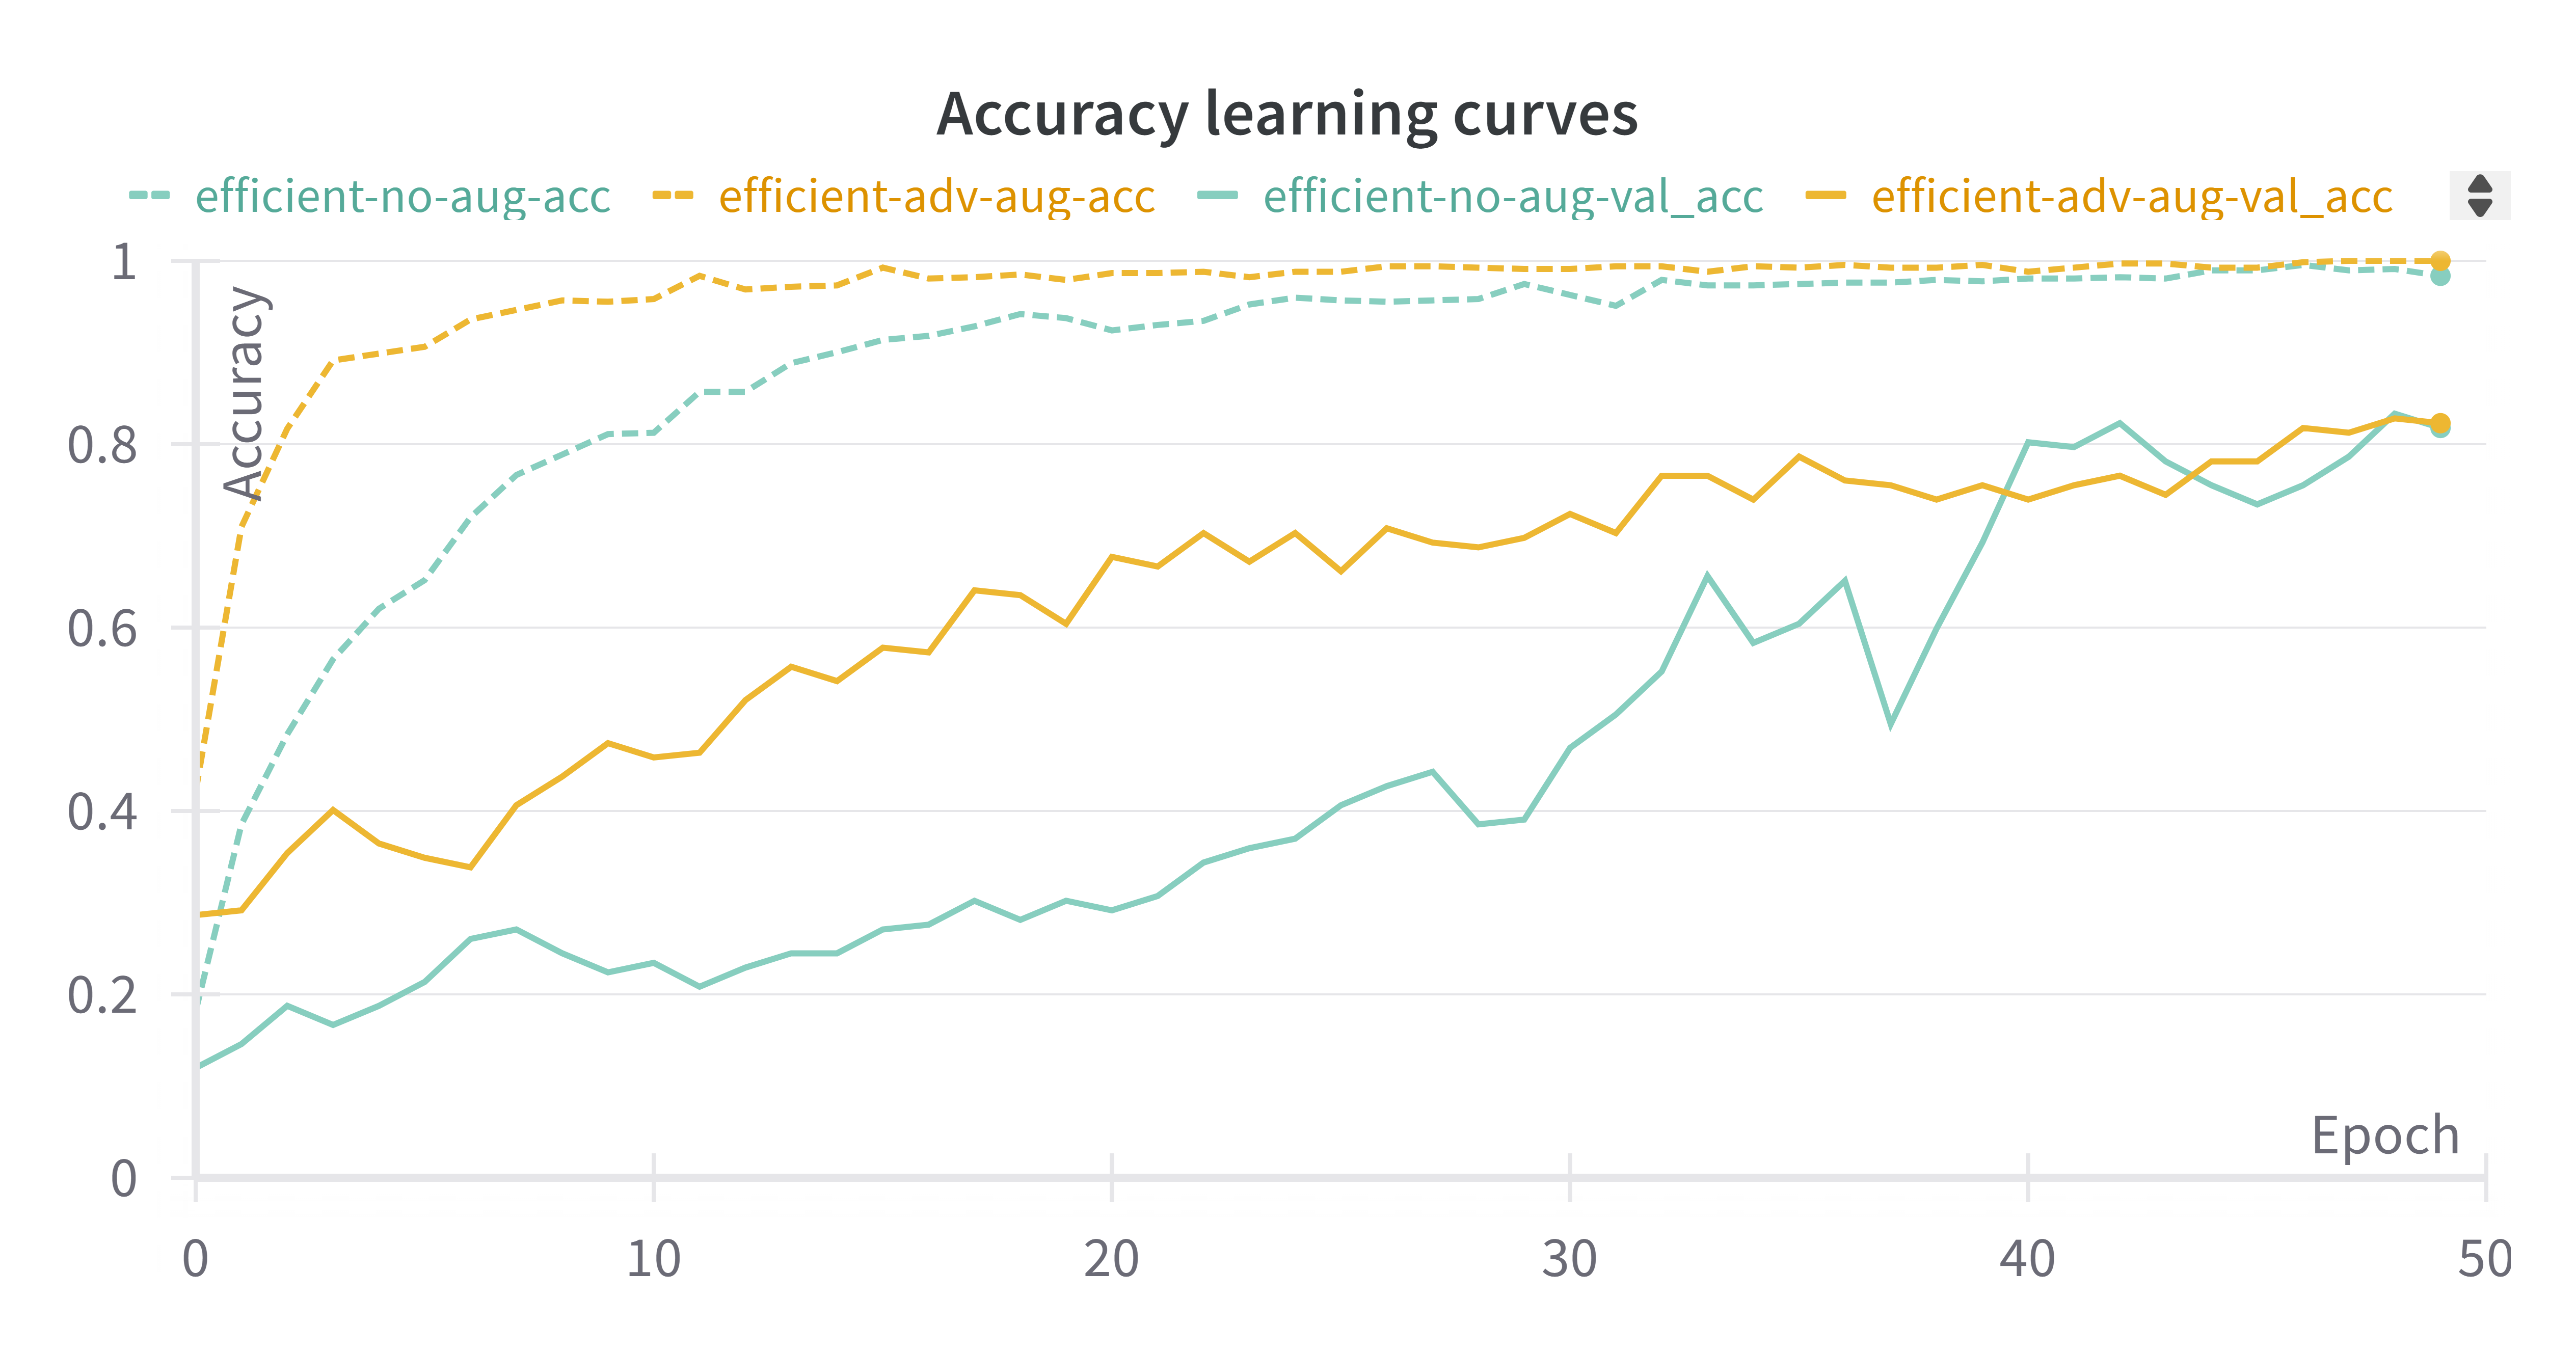
\includegraphics[width=0.8\textwidth]{Images/gtzan_plots/lc/efficient_acc_lc.png}
        \caption{Accuracy}
    \end{subfigure}
    \vspace{0.3cm}
    \hfill
    \begin{subfigure}{\textwidth}
        \centering
        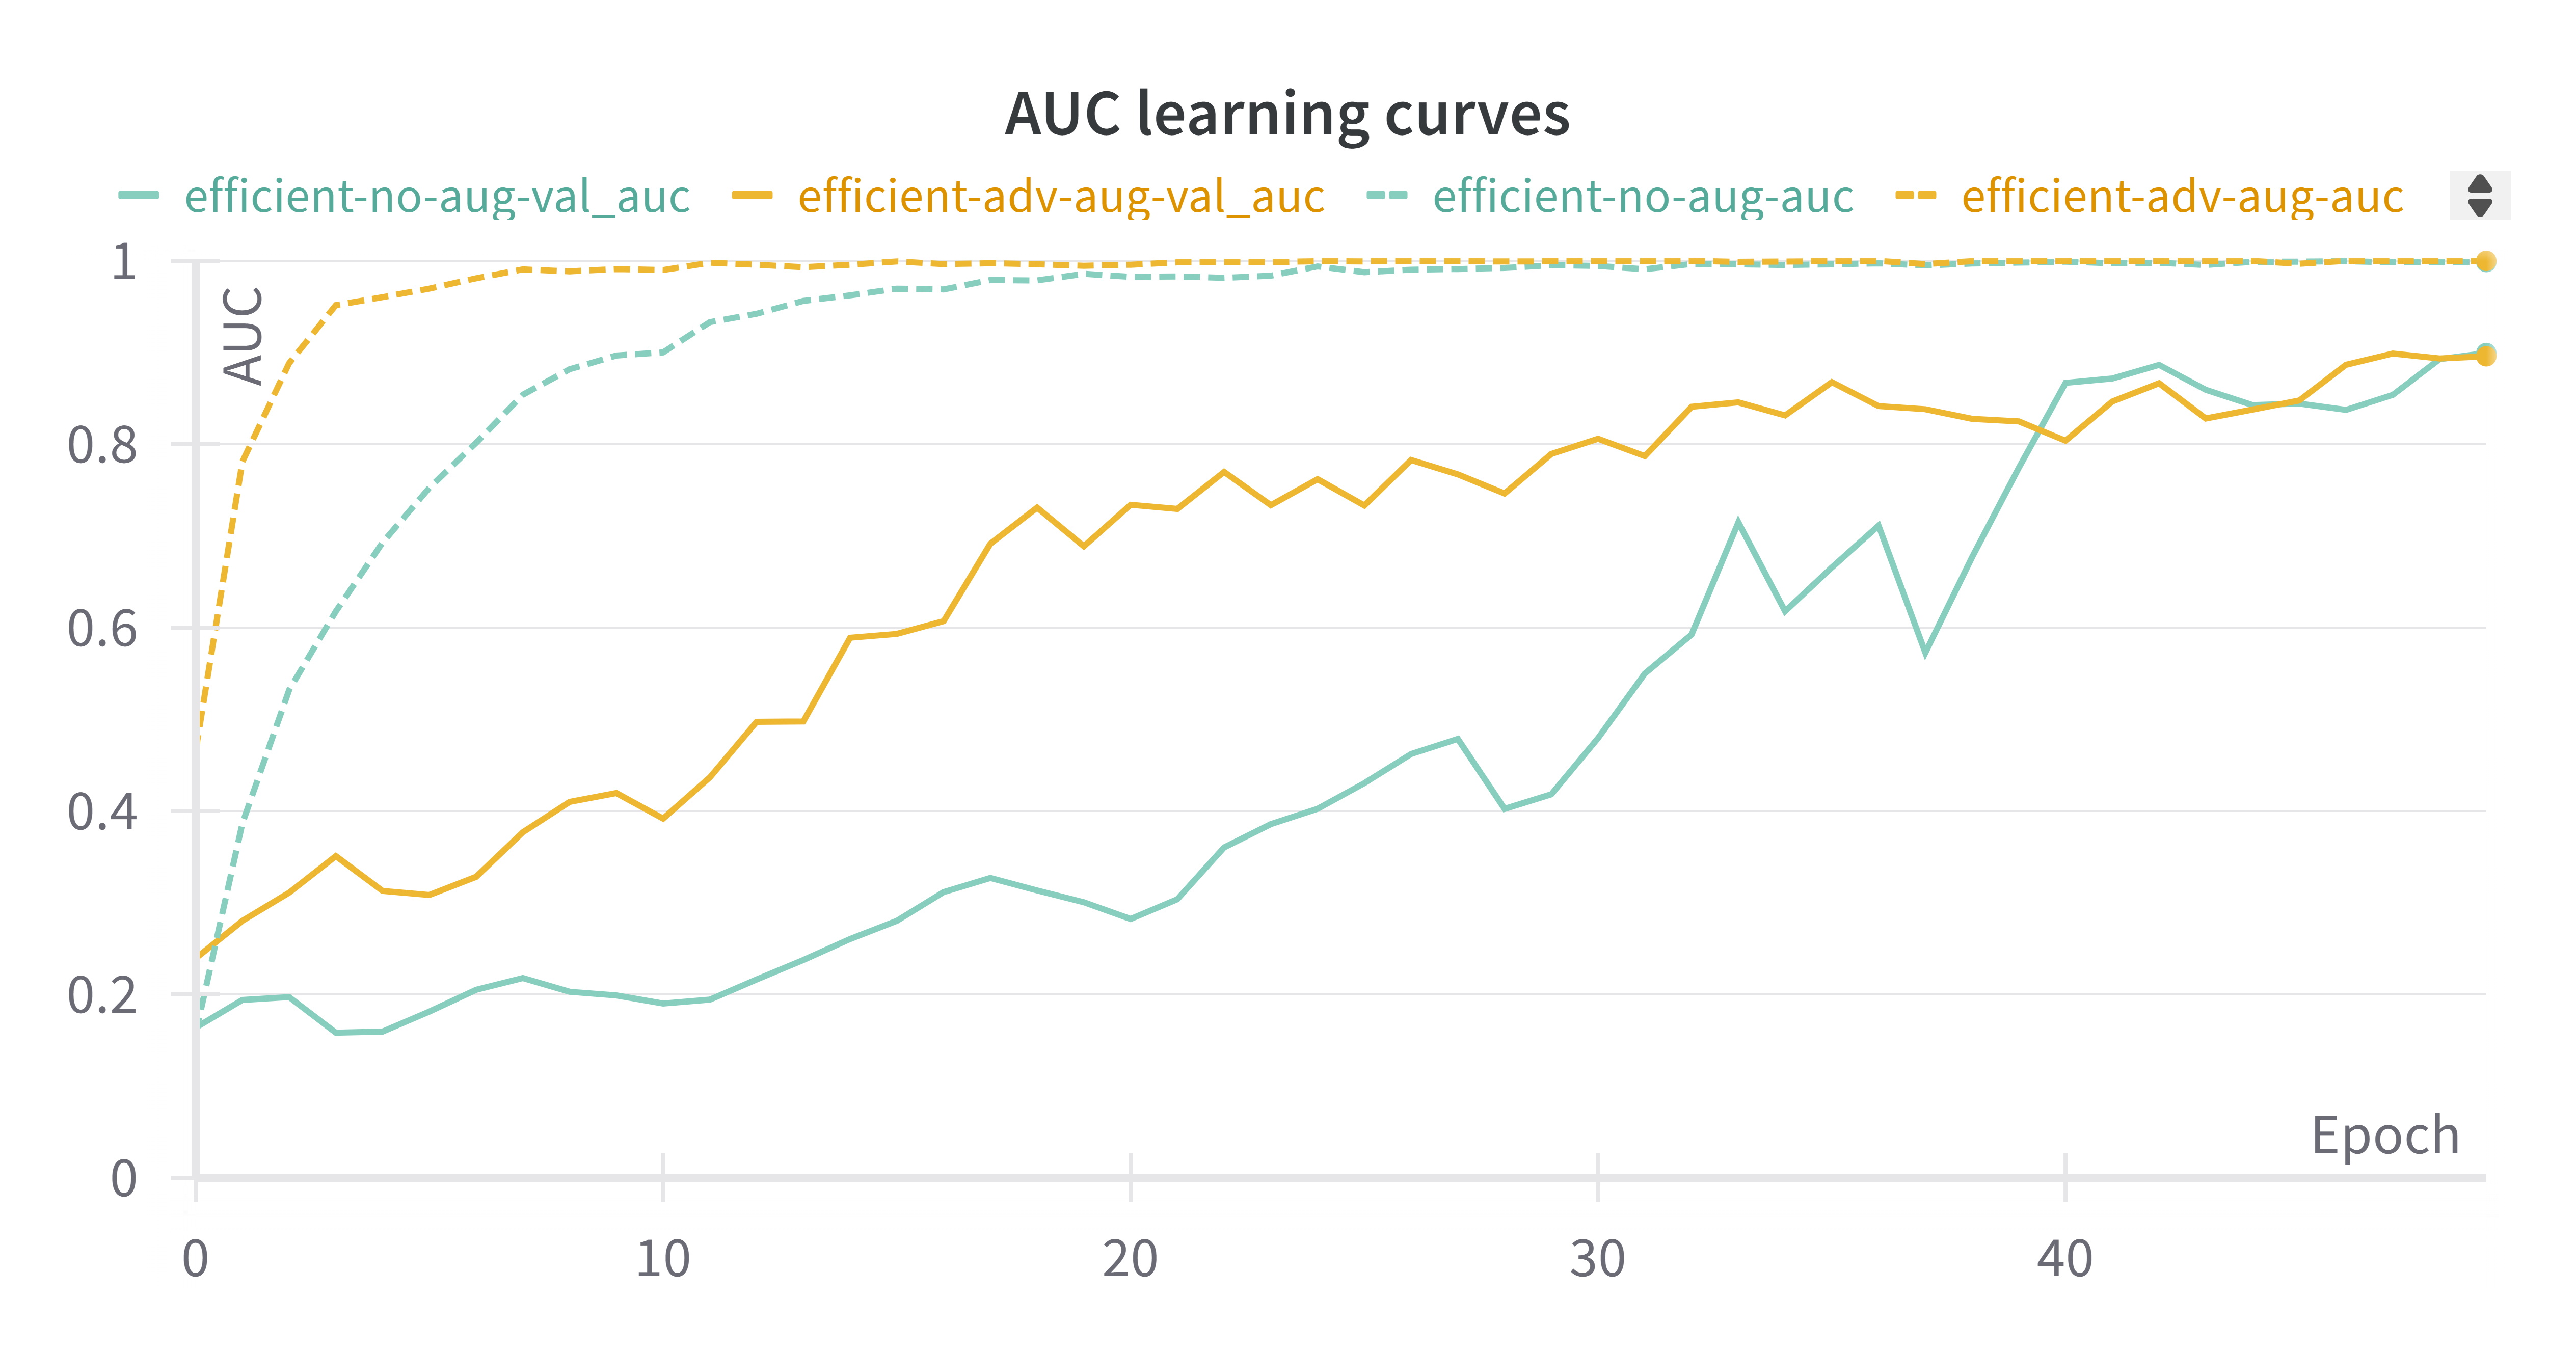
\includegraphics[width=0.8\textwidth]{Images/gtzan_plots/lc/efficient_auc_lc.png}\
        \caption{AUC}
    \end{subfigure}
    \vspace{0.3cm}
    \caption{Training and validation accuracy learning curves comparison for different augmentation types.}
    \label{fig:gtzanEfficientLC}
\end{figure}

Note that the validation accuracy for the model with augmentation is generally higher throughout the training process, even though it ends slightly lower than the model without augmentation. The augmented model performs exceptionally well on the test set, as shown in Table \ref{tab:gtzanEfficientnet}. This is likely because it consistently performed better throughout the entire training process, resulting in less random performance compared to the model without augmentation.

Interestingly, the model trained with augmentation shows a faster rise in both accuracy and AUC. This suggests that the augmentation techniques help the model learn the features of music more quickly, enabling it to classify music genres more effectively and efficiently. While a rapid increase in training accuracy might typically indicate overfitting, in this case, the validation accuracy also rises faster, suggesting that the model is not merely memorizing the training data. The validation accuracy and AUC for the model with advanced augmentation show a more gradual and consistent improvement, indicating better generalization. The test performance of the augmented model suggests that it has learned more robust features, leading to higher accuracy and AUC on unseen data.

\begin{table}[h!]
\centering
\caption{EfficientNet metrics comparison for GTZAN dataset.}
\begin{tabular}{| >{\centering\arraybackslash}m{2.5cm} !{\vrule width 1.5pt} >{\centering\arraybackslash}m{1.0cm} | >{\centering\arraybackslash}m{1.0cm} !{\vrule width 1.5pt} >{\centering\arraybackslash}m{1.0cm} | >{\centering\arraybackslash}m{1.0cm} !{\vrule width 1.5pt} >{\centering\arraybackslash}m{1.0cm} | >{\centering\arraybackslash}m{1.0cm} !{\vrule width 1.5pt} >{\centering\arraybackslash}m{1.0cm}|}
\hline
\multirow{2}{*}{\textbf{Augmentation}} & \multicolumn{2}{c!{\vrule width 1.5pt}}{\textbf{Train}} & \multicolumn{2}{c!{\vrule width 1.5pt}}{\textbf{Val}} & \multicolumn{2}{c!{\vrule width 1.5pt}}{\textbf{Test}} \\
\cline{2-7}
 & \textbf{Acc} & \textbf{AUC} & \textbf{Acc} & \textbf{AUC} & \textbf{Acc} & \textbf{F1} \\
\hline
no-aug & 99.11 & 0.999 & 83.33 & 0.893 & 76.77 & 75.84 \\
\hline
advanced & 99.55 & 0.996 & 82.81 & 0.894 & 91.92 & 91.64 \\
\hline
\end{tabular}
\label{tab:gtzanEfficientnet}
\end{table}

Similar to the observations with the Flowers 102 dataset, \textit{ResNet} architectures benefited more from augmentation than \textit{EfficientNet}. This makes these conclusions consistent and underscores the effectiveness of data augmentation techniques in improving model performance for \textit{ResNet} architectures compared to \textit{EfficientNet}.

Confusion matrices are shown in Figure \ref{fig:cmGTZAN}. Without data augmentation, the model performs perfectly for classical, jazz, and metal music. However, it struggles with several genres, including blues, disco, and country, which are frequently confused with other genres. With data augmentation, the model's performance improves significantly. It achieves 100\% accuracy not only in classical, jazz, and metal but also in country music. Additionally, it reaches 90\% accuracy in pop, reggae, and hip-hop. The worst performance is observed in rock and disco music. Disco is often confused with pop music, which makes sense because pop is a very general genre and can sound similar to disco. Rock, which is generally hard to define due to its many subtypes, is frequently misinterpreted as pop, metal, or country.

\begin{figure}[h!]
    \centering
    \begin{subfigure}[b]{0.6\textwidth}
        \centering
        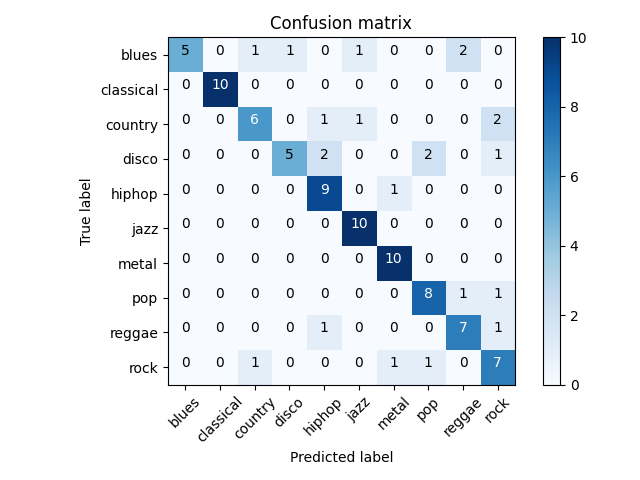
\includegraphics[width=\textwidth]{Images/gtzan_plots/cm/cm_gtzan_no_aug.png}
        \caption{Without augmentation}
    \end{subfigure}
    % \hfill
    \begin{subfigure}[b]{0.6\textwidth}
        \centering
        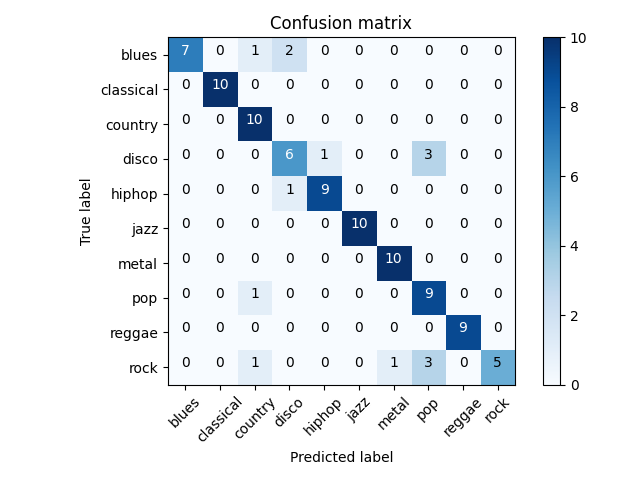
\includegraphics[width=\textwidth]{Images/gtzan_plots/cm/cm_gtzan_aug.png}
        \caption{With advanced augmentation}
    \end{subfigure}
    \caption{Confusion matrices calculated on the test set of the GTZAN dataset.}
    \label{fig:cmGTZAN}
\end{figure}

\newpage

\subsection{GAN Augmentation}

In this subsection, the concept of data augmentation using GANs is discussed. While GANs are a powerful tool for generating synthetic data that can enhance machine learning models, conducting such experiments is both \textbf{time} and \textbf{resource-consuming}. Due to these constraints, I did not perform most of these experiments myself. Instead, I focused on a comprehensive analysis of selected scientific studies conducted by other researchers in this field. This comparative approach provides greater \textbf{scientific value} and allows for the drawing of common conclusions, which will be discussed in the subsequent section.

The first network architecture explored was \textbf{Data Augmentation Generative Adversarial Networks (DAGAN)}, as detailed in the referenced paper~\cite{DAGANPaper}. What distinguishes DAGAN is its departure from conventional methods of image generation. Unlike traditional approaches, DAGAN does not rely on random noise for data creation. Instead, it uses images from the original dataset as described in Section \ref{ssec:augmentationGANs} and employs the \textit{UNet} architecture for lower space encoding. This methodology significantly \textbf{reduces the required training duration} and improves performance even in scenarios characterized by limited data availability. It also \textbf{reduces the variability} applied to the data, which is beneficial in data augmentation applications.

The authors tested this approach on three datasets. The Omniglot dataset contains $1623$ different characters from $50$ different alphabets. EMNIST (Extended MNIST) is a state-of-the-art dataset with handwritten letters and digits. VGG-Face dataset provides a large and diverse collection of face images for training deep learning models for face recognition. Authors limited number of samples, as shown in Figure \ref{fig:daganResults}

\begin{figure}[!h]
    \centering
    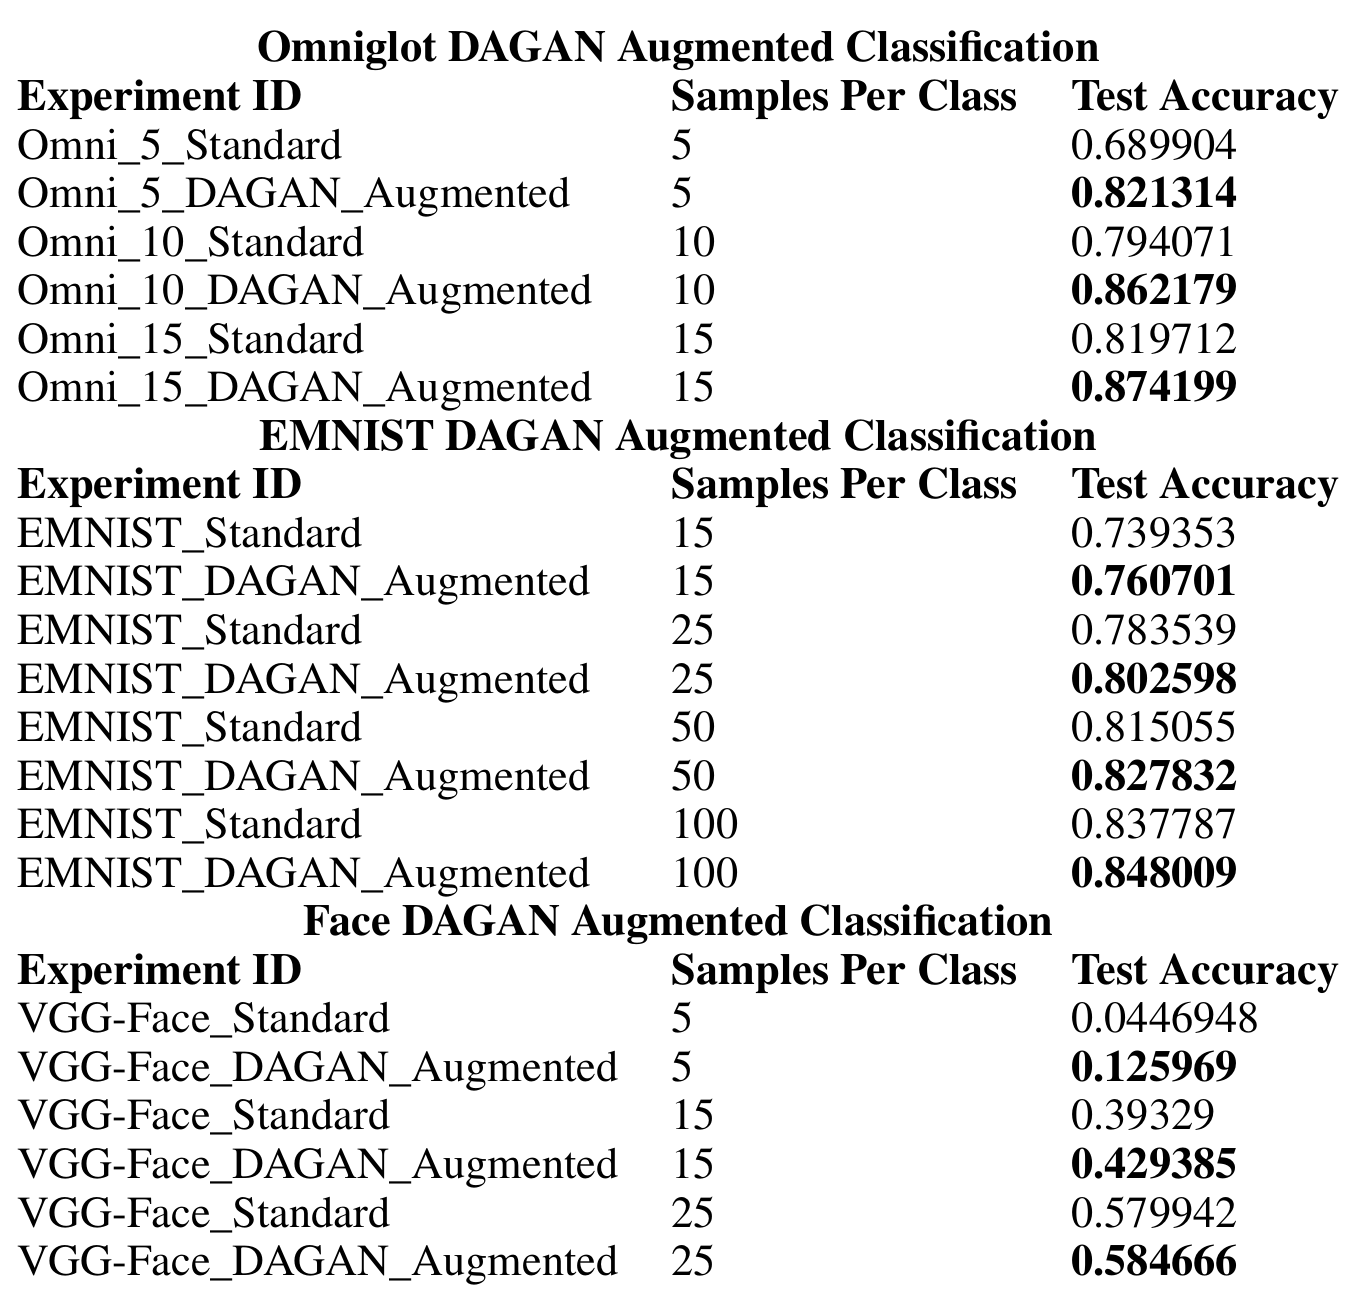
\includegraphics[width=0.7\textwidth]{Images/dagan_results.png}
    \caption{Results of DAGAN Augmentation~\cite{DAGANPaper}.}
    \label{fig:daganResults}
\end{figure}

The results indicate that using DAGAN for data augmentation consistently improves test accuracy across all three datasets (Omniglot, EMNIST, and VGG-Face) compared to traditional data augmentation ("Standard"). This improvement is more noticeable in experiments with fewer samples per class, highlighting DAGAN's significant influence on smaller datasets. The consistent improvement in test accuracy across various sample sizes demonstrates the effectiveness of DAGAN in generating useful synthetic data, particularly in scenarios with limited data availability.

On the other hand, even though the authors did not provide information about the training time, I checked it myself by running the code attached to the paper. Training DAGAN for $50$ epochs on the smallest dataset (Omniglot) takes approximately 3-4 hours when the \textit{Tesla T4 GPU} is utilized. The training time is likely to be even longer for the VGG-Face dataset, which contains higher-resolution images. This indicates that while DAGAN offers significant benefits in terms of improved accuracy, it also requires substantial computational resources and time, especially for higher-resolution datasets. Additionally, the authors used quite simple architecture as a classificator. Implementing \textit{ResNet50} or another state-of-the-art network pre-trained on the \textit{ImageNet} dataset could yield even better results than data augmentation.

Interesting experiments were also conducted in the article~\cite{CycleGANBreastCancer}. By using the \textbf{CycleGANs},  mammograms with \textbf{breast} masses were synthesized from CT images of \textbf{lung} nodules. This approach leveraged the common characteristics of tumor-like lesions across \textbf{different organs}.  

\begin{figure}[!h]
    \centering
    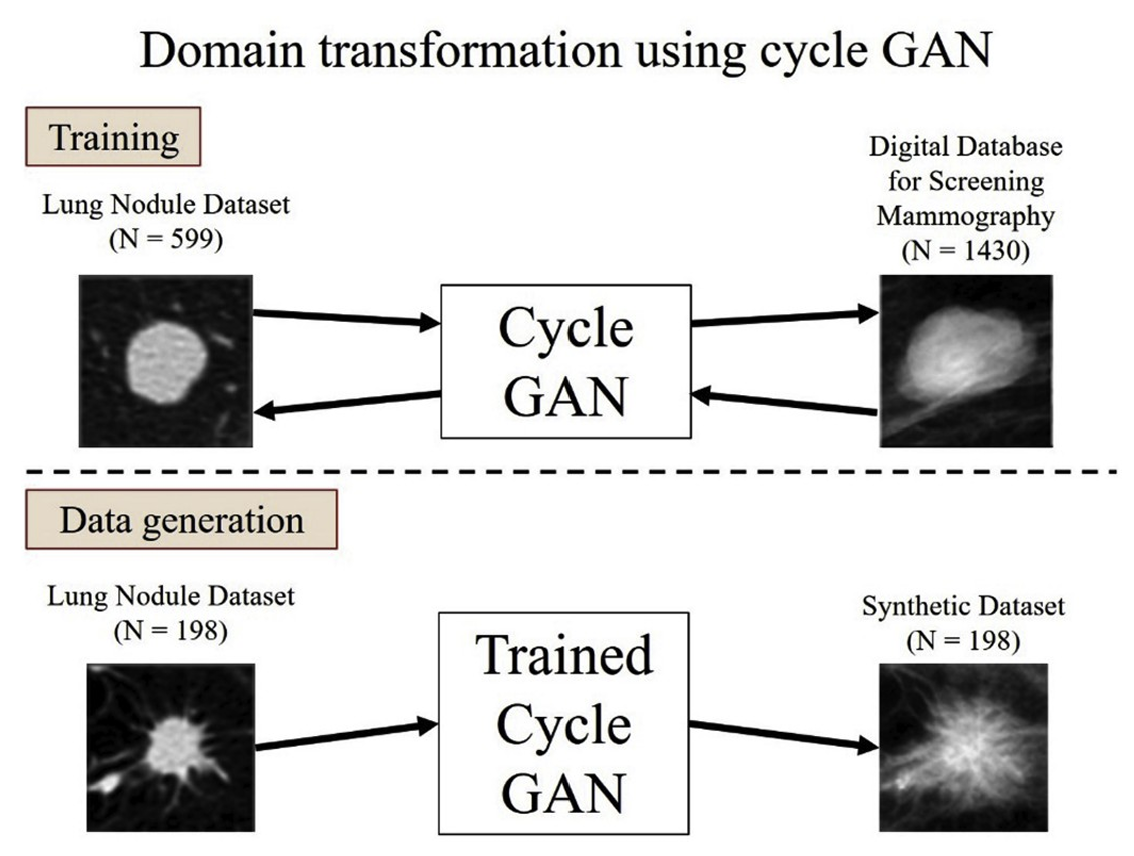
\includegraphics[width=0.8\textwidth]{Images/cycleImageGen.png}
    \caption{GAN training and generation framework. The lung nodule dataset and open-source digital mammography database were used to train a cycle GAN and generate synthetic data~\cite{CycleGANBreastCancer}.}
    \label{fig:overaugLC}
\end{figure}


The network architecture included two generators, each with convolutional layers followed by resnet blocks. There were also two discriminators, each consisting of convolutional layers. The input and output image size for the generators is $256$ x $256$ pixels. Unlike traditional GANs that take random noise as input, CycleGANs take images directly from two distinct domains as input: one from the source domain and one from the target domain. This allows for more controlled and direct feature transfer between the images.

A 50-layer residual network (\textit{ResNet}) was trained to classify breast masses as benign or malignant. The input images were resized to $224$ x $224$ pixels. Public databases were utilized to enhance a small dataset. In this study, the open-access Digital Database for Screening Mammography (DDSM) was used for two main purposes: to pre-train the classification network for comparison with synthesized data results and to train the GAN.

The use of synthetic images for training a CNN to classify mammographic masses was explored. Breast mass images synthesized from the CT lung nodule dataset were examined by experienced radiologist using a 10-point scale, where 1 and 10 corresponded with definitely fake and real. The ratings for real and synthetic data were 5.9 and 4.9, respectively.

\begin{table}[ht]
\centering
\caption{Validation and test accuracies and the AUC for classification of benign and malignant breast masses.}
\begin{tabular}{|c|c|c|c|c|}
\hline
Conditions & \makecell{ImageNet\\Pretrained} & \makecell{Validation\\Accuracy} & \makecell{Test\\Accuracy} & \makecell{Test\\AUC} \\ \hline
Original dataset   &  No                   & 67.9\%              & 65.7\%        & 0.724   \\ \hline
Original with rotations and flips   &  No                   & 70.8\%              & 67.1\%        & 0.741   \\ \hline
Original with rotations and flips  & Yes                   & 80.5\%              & 79.2\%        & 0.869   \\ \hline
Original + GAN Synthetic   & Yes                   & 81.3\%              & 81.4\%        & 0.884   \\ \hline
Original Augmented + DDSM Pretrained   & Yes                   & 82.3\%              & 80.9\%        & 0.886   \\ \hline
\end{tabular}
\label{tab:cycleGANBreast}
\end{table}

Table \ref{tab:cycleGANBreast} shows that the model benefits the most from using the version pre-trained on the \textit{ImageNet} dataset. The study showed that the use of synthetic data yielded comparable results to using digitized mammography data for pretraining, meaning that in the absence of public datasets, this proposed method could serve as an alternative for generating training samples.

By employing this method, it becomes possible to share samples of mass-like lesions across different organs. Additionally, synthesized images with diverse shapes and textures can be used to create realistic samples similar to study cases through domain transformation. A key benefit of using the CycleGAN is its ability to function without paired ground truth images. Consequently, this allows for the synthesis of breast lesion images based on lung lesions.

Despite all these advantages, the improvement is minimal, and a radiologist was needed to evaluate the generated images. It means that training the network and generating new images is time-consuming and requires a significant amount of work. Consequently, the practical benefits of this approach are limited and may not justify the extensive effort required.

\textbf{DCGANs} were also used for data augmentation by Salehinejad et al.~\cite{DCGANImbalanced} to generate chest radiographs with pathologies to address \textbf{dataset imbalance}. The dataset comprised 15,781 normal examples, 17,098 instances of cardiomegaly, 14,510 cases of pleural effusions, 5,018 examples of pulmonary edema, and only 4,013 instances of pneumothorax. These images were exported and anonymized as PNG files after being down-sampled to $256$×$256$ pixels, ensuring a balance between maintaining resolution and reducing computational complexity. For all experiments, 1,000 real chest X-rays of each class were selected for validation, and an identical number was selected for model testing.

A team of radiologists eliminated inappropriate generated chest X-rays from the respective class directories. To maintain a balanced training dataset across different classes, the DCGAN was trained with a dataset consisting of 2,000 chest X-rays per class. 

\begin{figure}[!h]
    \centering
    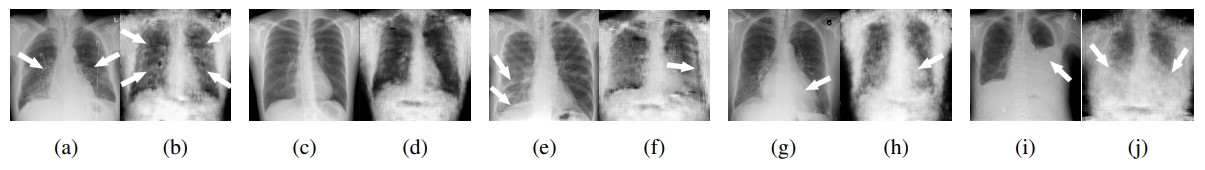
\includegraphics[width=0.9\textwidth]{Images/dcganAugmentation.jpg}
    \caption{Examples of real (R) and synthesized (S) chest X-rays: (a) Pulmonary Edema-R; (b) Pulmonary Edema-S; (c) Normal-R; (d) Normal-S; (e) Pneumothorax-R; (f) Pneumothorax-S; (g) Cardiomegaly-R; (h) Cardiomegaly-S; (i) Pleural Effusion-R; (j) Pleural Effusion-S. The white arrow indicates the pathological condition~\cite{DCGANImbalanced}.}
    \label{fig:dcganAug}
\end{figure}

The classifier was similar to AlexNet but with different kernel sizes. The number of images generated was huge. It amounted to more than 28,000 for the least numerous class. As we can observe in Figure~\ref{fig:DCGANResults}, the augmentation led to an increase in validation accuracy from 71\% to 92\%.


\begin{figure}[!htb]
    \centering
    \begin{subfigure}[b]{0.45\textwidth}
        \centering
        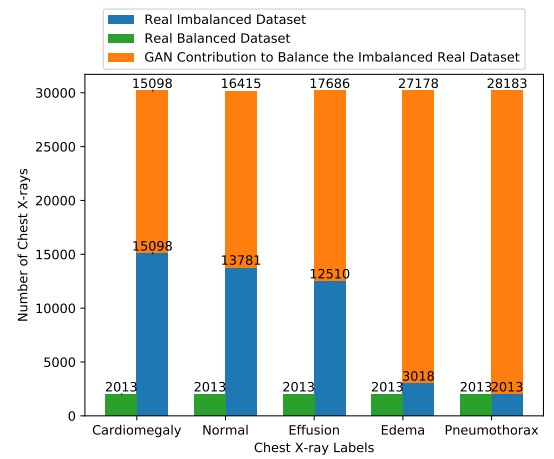
\includegraphics[width=\textwidth]{Images/dcganImbalanced.jpg}
        \caption{Dataset sizes}
    \end{subfigure}
    \vspace{0.3cm}
    \hfill
    \begin{subfigure}[b]{0.45\textwidth}
        \centering
        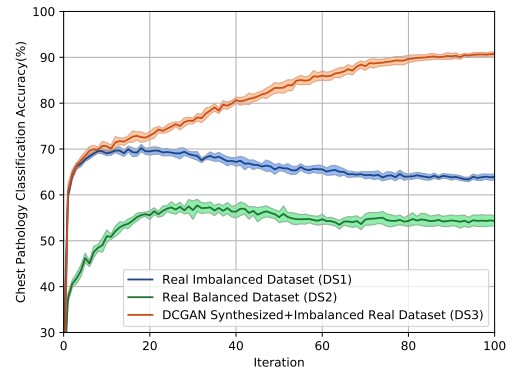
\includegraphics[width=\textwidth]{Images/dcganLC.jpg}
        \caption{Learning curves}
    \end{subfigure}
    \vspace{0.3cm}
    \caption{DCGAN augmentation results. Original dataset (blue), Balanced dataset (green), and GAN contribution to balance the dataset (orange)~\cite{DCGANImbalanced}.}
    \label{fig:DCGANResults}
\end{figure}

In another study, Frid-Adar et al.~\cite{Frid_Adar_2018} created synthetic images of liver lesions, including cysts, metastases, and hemangiomas, which improved classification sensitivity from $78.6$\% with regular augmentation to $85.7$\% when GANs were used for data augmentation. Radiologists evaluated these synthetic images, achieving about $60$\% accuracy in distinguishing 182 real and $120$ fake images.

On the other hand, Fedoruk et al.~\cite{CovidGAN} researched the effectiveness of GAN-based augmentation in classifying lung X-ray medical images, based on the \textbf{dataset size}. The findings shown in the Table \ref{table:augmentation} reveal that for medium and large datasets, GAN-based augmentation performs similarly to traditional augmentation methods. However, due to significant time and hardware demands, this method is not practical as the primary augmentation technique. In cases of smaller datasets, the GAN model failed to train sufficiently to generate useful training data. Despite this, the competitive performance of GAN with classical augmentation for larger datasets suggests a potential solution for the scarcity of medical data by sharing synthetic images instead of real ones.

\begin{table}[h!]
\centering
\caption{Accuracy of different augmentation pipelines for big dataset.}
\begin{tabular}{|l|c|}
\hline
\textbf{Augmentation pipeline} & \textbf{Accuracy} \\
\hline
No augmentation & 0.855 \\
\hline
Classic augmentation & 0.891 \\
\hline
GAN-augmentation & 0.871 \\
\hline
\end{tabular}
\label{table:augmentation}
\end{table}

\section{Interpretation of Results}
\label{sec:resultsInterpretation}


In this section, the findings from all experiments presented in this chapter are summarized. The focus was on providing a broader perspective on the results, rather than on specific numerical values. This approach aims to highlight the overall effectiveness and potential applications of different data augmentation techniques across various scenarios.

In the experiments with the \textbf{Flowers 102 dataset}, the performance of the state-of-the-art \textit{ResNet50} model without data augmentation initially showed overfitting. Testing individual traditional transformations led to improvements in validation and test results, with cropping and rotations being the most effective. Combining all traditional augmentations additionally enhanced the results, but the best performance was achieved when traditional techniques were combined with \textit{MixUp} and \textit{CutMix}. These experiments were repeated three times, and consistent results were obtained, demonstrating that the network's already high performance can be further improved by applying augmentations. \textit{MixUp} and \textit{CutMix} had the most significant influence on the training curve, which was lower than the validation curve for these techniques. While saliency maps without and with augmentations appeared very similar, the network trained on augmented data sometimes focused on more relevant parts of the input image, particularly when it avoided mistakes.

In the experiments on the \textbf{Flowers 102 dataset under limited data conditions} with $5$, $10$, and $20$ samples per class, it was observed that the fewer data available, the more significant the influence of data augmentation. Although no augmentation type provided as substantial improvement as doubling the number of examples, advanced augmentation achieved almost as good results. Training a network requires more epochs to stabilize with fewer data samples. With advanced augmentation applied to the dataset with 20 samples per class, the results were nearly as good as those obtained from the full dataset without augmentation, which is almost three times larger. For the medium dataset with 10 samples per class, saliency maps showed a marked difference between models trained with and without augmentation. When advanced augmentation was applied, the model focused on much more important parts of the input images, with areas of interest becoming more human-like.

In the experiments with the \textbf{GTZAN dataset} (audio files), the biggest challenge was that some augmentations had to be applied at the audio wave level. This requirement significantly slowed down the training process because the Mel Spectrogram transformation needed to be performed at every step of each epoch. Without augmentation, the model achieved perfect accuracy on the training data within a few epochs. However, with augmentation, the model did not reach perfect performance on the training data, even by the end of the training. This continuous learning process throughout all epochs, driven by augmentation, led to a significant improvement in accuracy. Additionally, augmentation enhanced other performance metrics, including F1 score, precision, recall, and confusion matrices, indicating a more robust and generalizable model.

In the experiments involving the \textbf{\textit{EfficientNetB0}} architecture on both the GTZAN and Full Flowers 102 datasets, validation accuracy remained nearly the same with and without augmentation. However, test metrics showed slight improvements with augmentation. This suggests that while \textit{EfficientNetB0}, a more optimized network, benefits somewhat from augmentation, the impact is less visible compared to architectures like \textit{ResNet}, which has more parameters. The \textit{ResNet's} higher parameter count likely contributes to its greater vulnerability to overfitting and, consequently, its more significant gains from data augmentation. In contrast, \textit{EfficientNetB0's} design reduces overfitting naturally, resulting in less visible improvements from augmentation.

It has been observed that data augmentation does not always result in improvements. When excessive transformations like rotating flowers upside down, applying high levels of contrast changes, or using overly large zooms are applied to the dataset with high probabilities, there is a significant decrease in accuracy. This underscores the importance of applying data augmentation techniques carefully and intelligently. Over-augmenting by using extreme transformations can distort the data too much, leading to poor model performance. 


It is worth noting that \textbf{maintaining the same accuracy} while adding noise or other augmentations is a positive outcome. Often, images in validation and test sets are centered, have similar backgrounds, are taken by the same photographer, and have comparable quality to the training images. However, when our model encounters user-provided images taken with inferior cameras or from different angles, it will perform better if it has seen such variations during training. This exposure helps the model generalize better and handle real-world scenarios more effectively. That is why test or validation metrics do not necessarily have to rise, as they do not directly benefit from these transformations.

The concept of \textbf{utilizing Generative Adversarial Networks (GANs)} for data augmentation initially seemed promising, offering the potential to enhance the diversity and quality of training datasets for image classification. However, as I started experimental implementations, it became evident that the application of GANs for data augmentation was not as straightforward as expected.

First, when we want to use Generative Adversarial Networks for augmenting datasets in classification tasks, we cannot use any \textbf{architecture type} we wish since we need the output data to be labeled. Therefore, we need to use one of the architectures listed in Section \ref{ssec:typesOfGANs} but not all of them must be suitable for our problem. 

Once an architecture has been selected, another critical consideration emerges: \textbf{training time}. The process of training a proficient generative model is notably time-intensive, often extending over hours or even days, surpassing the duration typically required for training classification models. Furthermore, it requires a \textbf{large amount of computational resources}, which adds to the complexity of the training process.

\textbf{Data size and quality} are another obstacles preventing GANs' development for data augmentation. When dealing with small datasets or low-resolution images, training GANs can be impractical due to the substantial amount of high-quality data they require to generate satisfactory results. As a result, the volume of data needed to train GANs effectively often overlaps with what would already be sufficient for training a competent classifier.

Despite the challenges listed above, there are certain cases where utilizing GANs is highly beneficial. One such example is the \textbf{DAGAN architecture}, which shows great promise due to its relatively lower training requirements. DAGAN takes information directly from the dataset as input, making it particularly well-suited for classification tasks. This approach allows for efficient and effective augmentation, helping to enhance the performance of models without the extensive computational overhead typically associated with GAN training.

Another case where GANs prove to be very helpful is with \textbf{imbalanced datasets}. By generating synthetic samples for the least numerous classes, GANs can improve the performance of classifiers. This approach was demonstrated in one of the experiments, where the addition of GAN-generated samples led to more balanced datasets and significantly enhanced classification performance.

Another general category where GANs can be useful is \textbf{medical data}. It is often challenging or impossible to gather large medical datasets due to privacy and legacy issues. In such cases, GANs can be employed to generate new images, which can then be reviewed by radiologists to ensure quality. Additionally, as demonstrated in experiments, it is possible to transfer knowledge from one organ to another, such as adding a tumor from the lungs to the breast. While this process is time-consuming, it sometimes proves to be the only viable option for augmenting medical datasets and improving model training.

In summary, when data augmentation is applied correctly, significant improvements in model performance can be observed. Even traditional, simple methods like cropping and rotations can greatly enhance validation and test results. Advanced techniques such as \textit{MixUp} and \textit{CutMix} further improve outcomes. GANs, while requiring careful consideration of architecture, training time, and data quality, also offer substantial benefits in specific cases such as addressing data imbalance and augmenting medical datasets. Thus, when used properly, both traditional and GAN-based augmentation techniques can considerably boost the robustness and accuracy of machine learning models.